% Rebuilt with original Frontiers supplementary template files and embedded full supplementary tables on 2026-07-07.
\documentclass[utf8]{frontiers_suppmat}
\usepackage{url,hyperref,lineno,microtype}
\hypersetup{hidelinks}
\usepackage[onehalfspacing]{setspace}
\usepackage{graphicx}
\usepackage{booktabs,longtable,array,pdflscape}
\newcolumntype{L}[1]{>{\raggedright\arraybackslash\hspace{0pt}}p{#1}}
\setlength\LTleft{0pt}
\setlength\LTright{0pt}
\emergencystretch=3em
\sloppy

\begin{document}
\onecolumn
\firstpage{1}

\title[Supplementary Material]{{\helveticaitalic{Supplementary Material}}}

\maketitle

\section*{Supplementary Material Overview}
This supplementary material contains Supplementary Figures S1-S3 and complete embedded display versions of Supplementary Tables 1-11. The original CSV files, the combined Excel workbook and the figure source-data folder are included with the review package as machine-readable source files.

\section*{Supplementary Figures}
\clearpage
\begin{figure}[h!]
\begin{center}
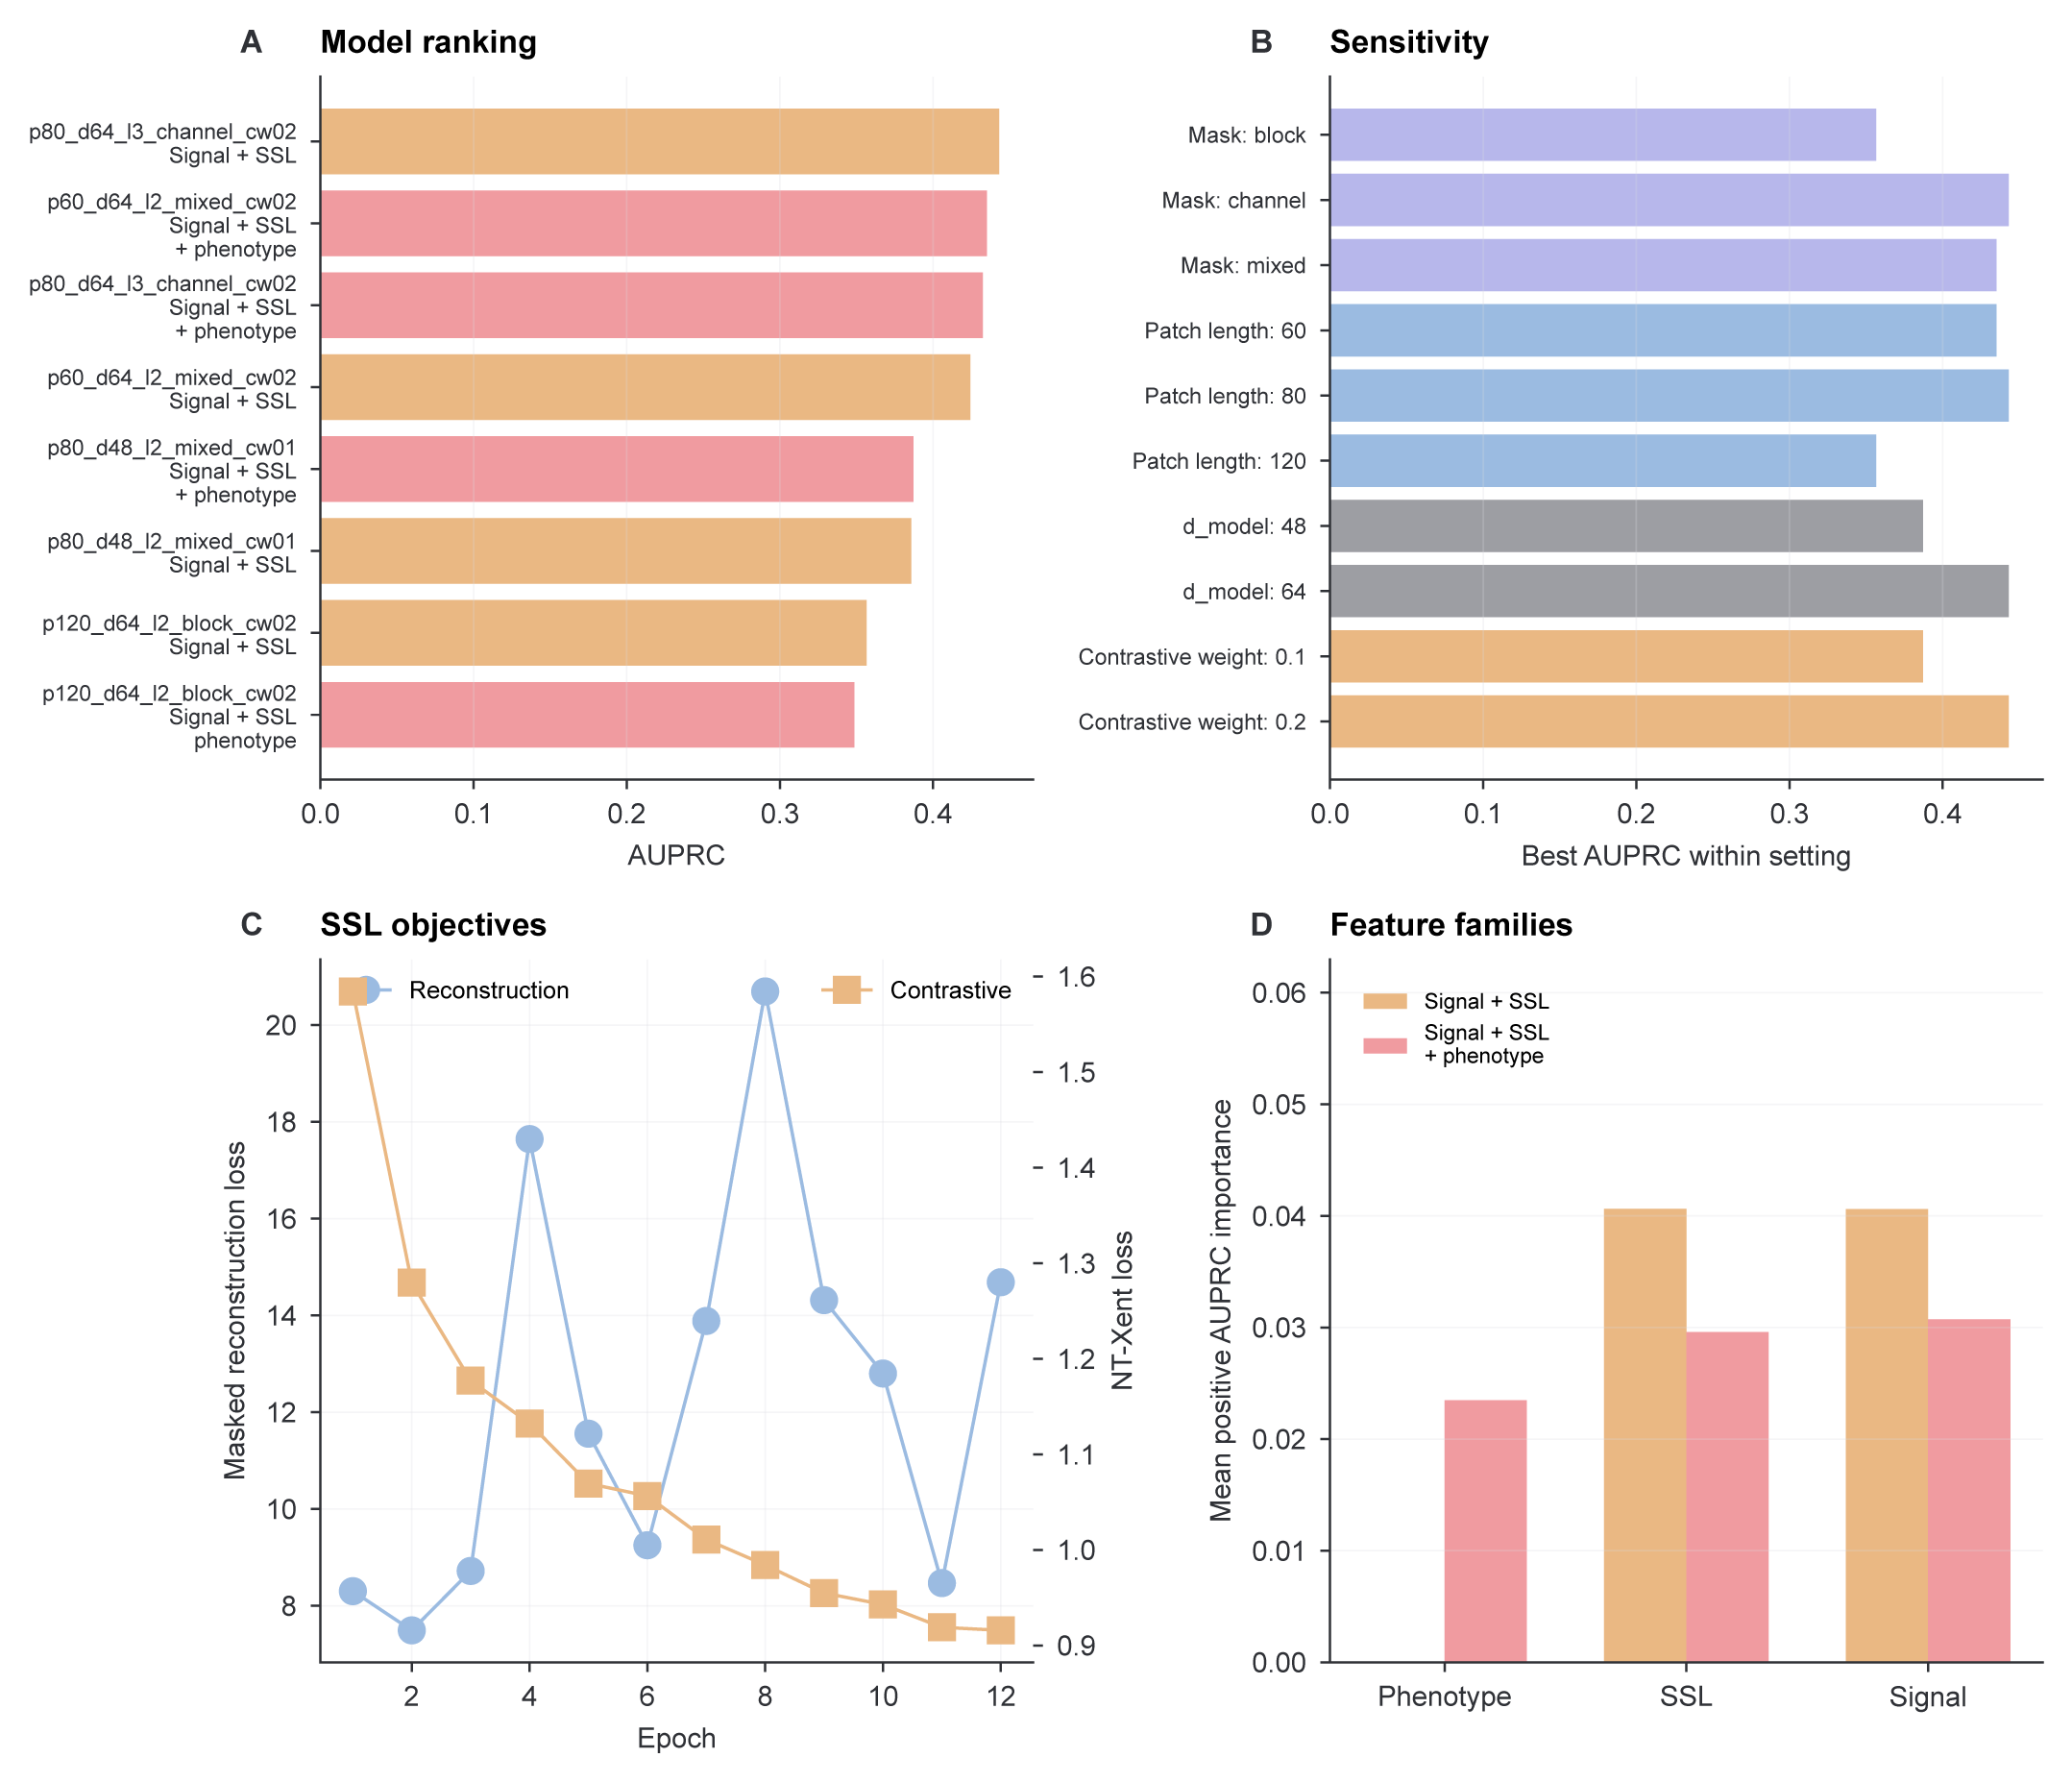
\includegraphics[width=\textwidth]{figures/Supplementary_Figure_S1_model_selection_and_sensitivity.png}
\end{center}
\caption{\textbf{AI model-selection and sensitivity panels for the transformer phenotyping workflow.} Supplementary analyses of the self-supervised AI method layer. (A) Exploratory transformer configuration and feature-set combinations ranked by held-out AUPRC. (B) Sensitivity summary across masking strategy, patch length, model dimension and contrastive objective weight, using the best AUPRC observed within each setting. Because these panels use held-out performance for method exploration, they should not be interpreted as a locked independent model-selection experiment. (C) Training-objective trace for a selected-architecture refit, showing masked reconstruction loss and NT-Xent contrastive loss across epochs; the oscillating reconstruction trace was used for training-dynamics inspection only and did not determine downstream representation selection. (D) Feature-family contribution to AUPRC-based permutation importance for signal-plus-SSL and final phenotype-augmented models.}\label{fig:model_selection_sensitivity}
\end{figure}

\clearpage
\begin{figure}[h!]
\begin{center}
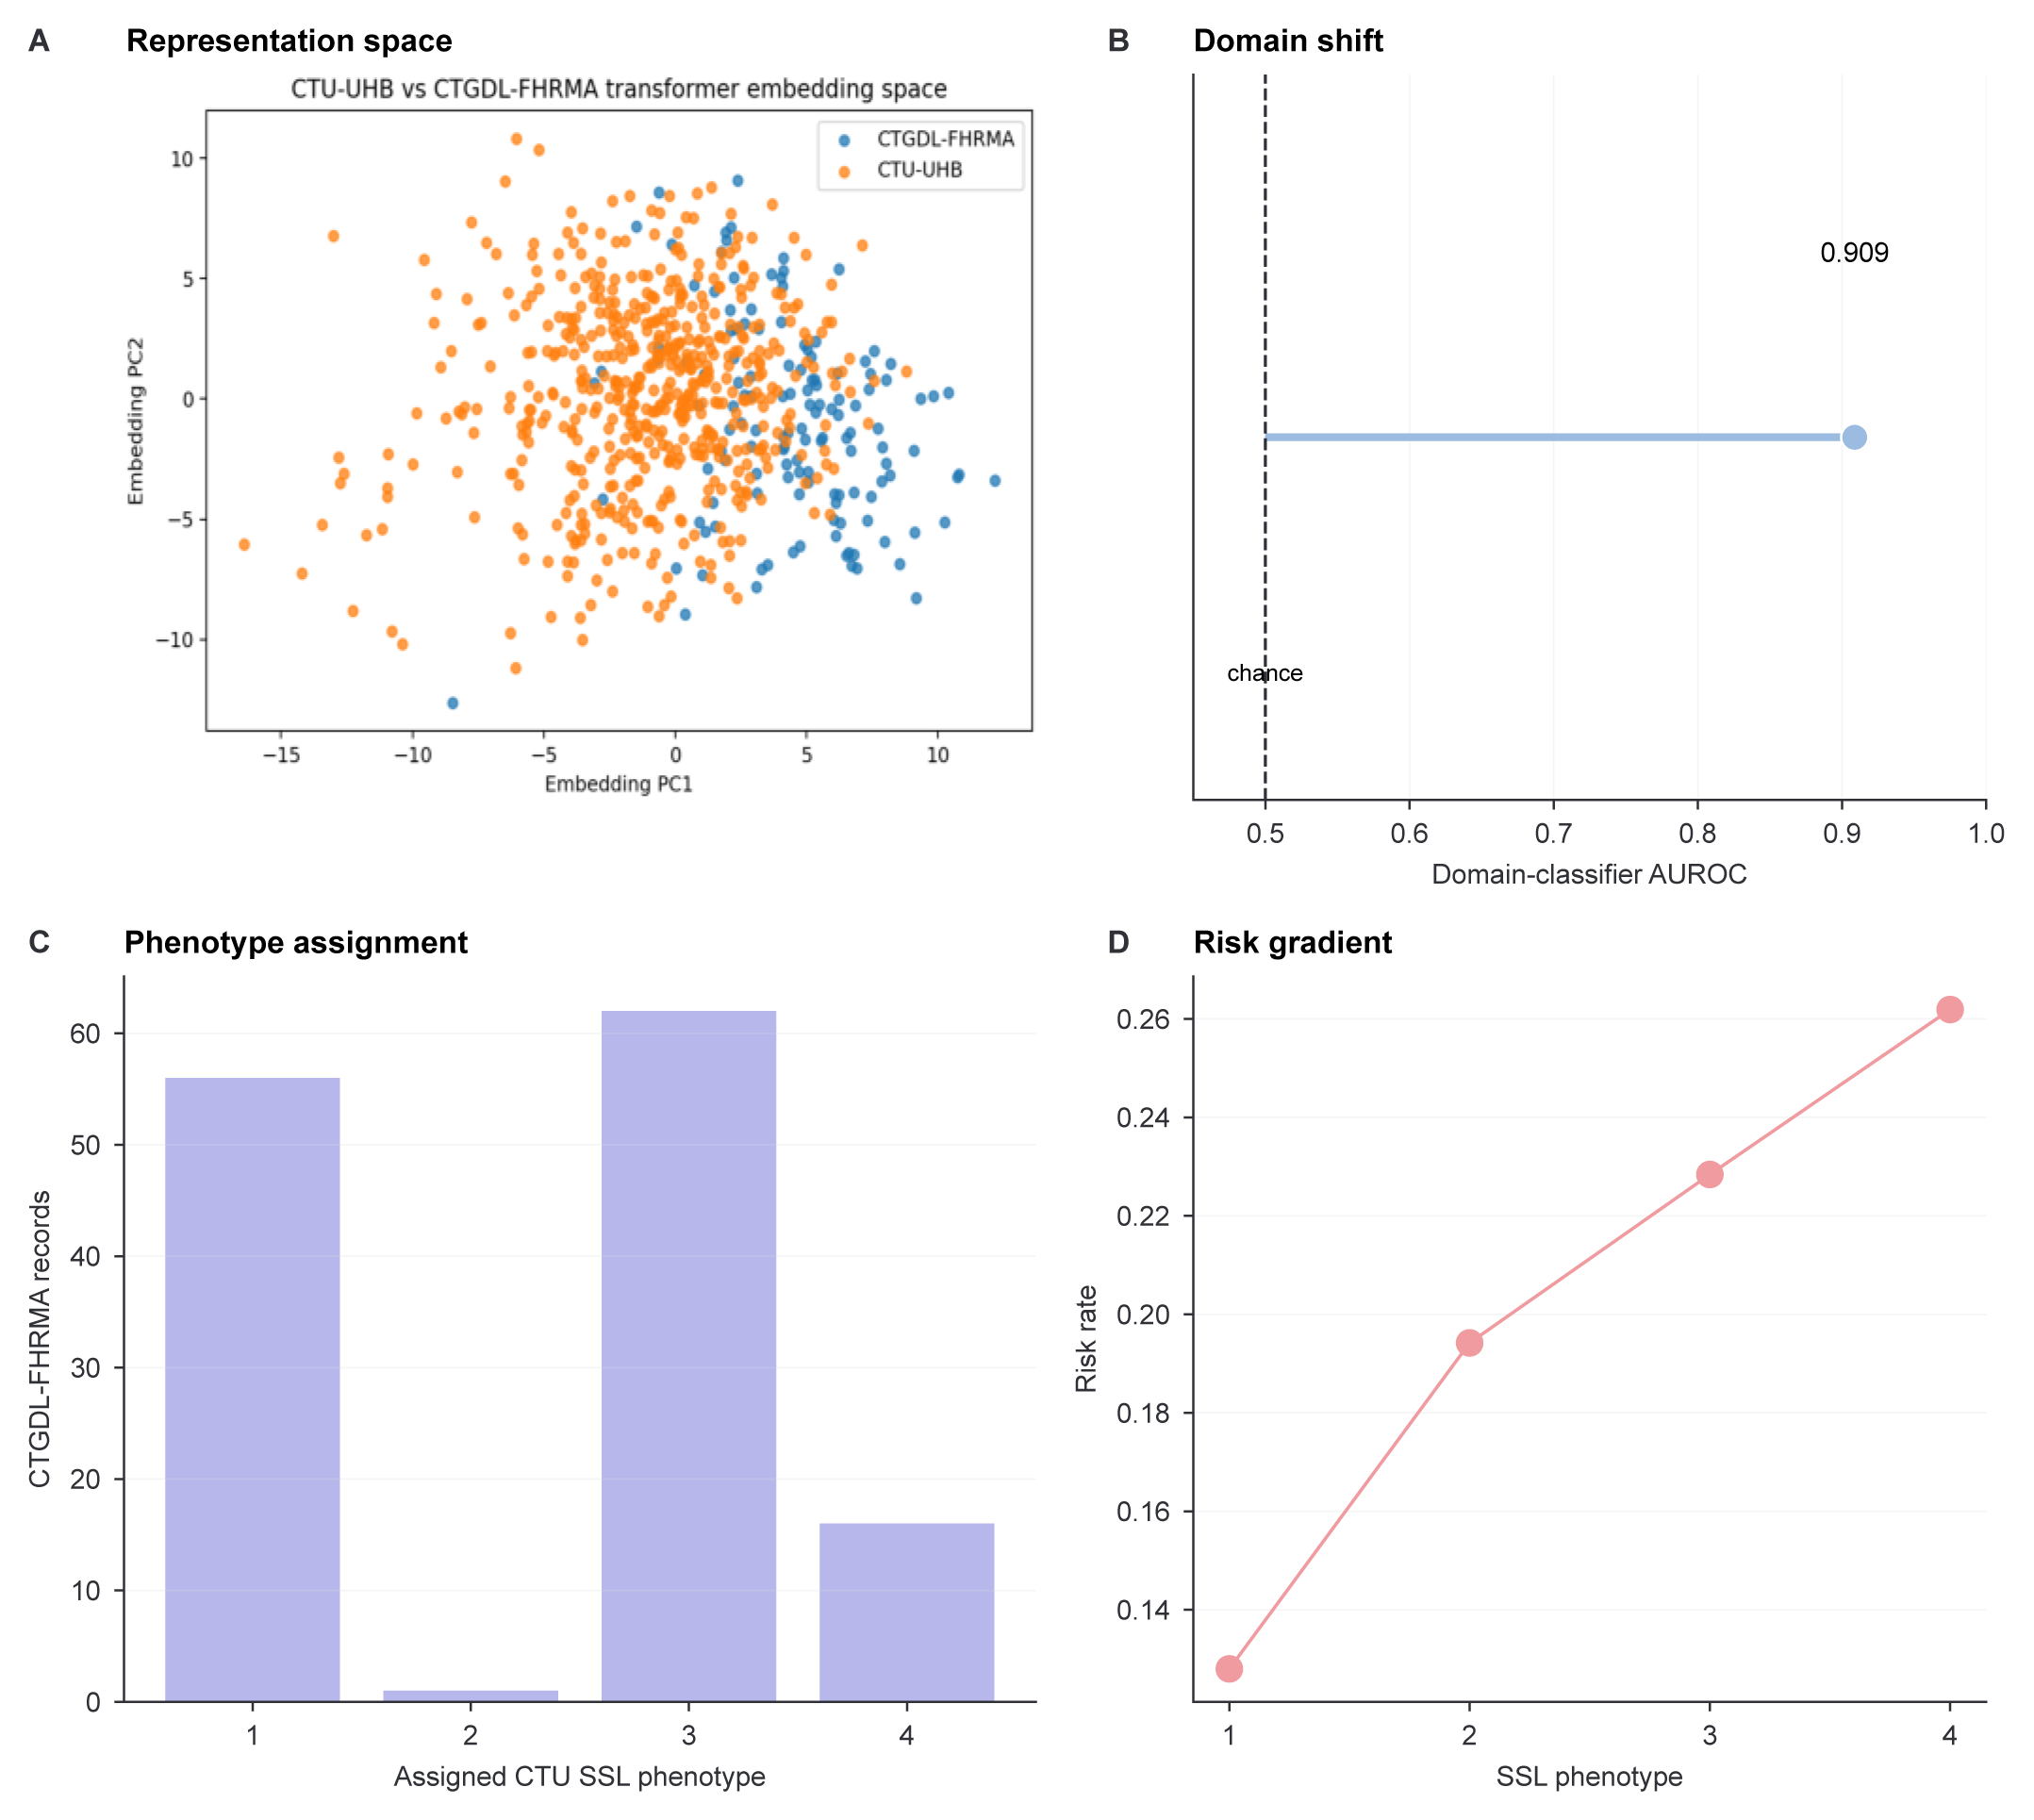
\includegraphics[width=\textwidth]{figures/Supplementary_Figure_S2_external_domain_shift.png}
\end{center}
\caption{\textbf{CTGDL-FHRMA supports external representation projection and domain-shift assessment.} External representation analysis using CTGDL-FHRMA records. Because external neonatal outcome labels were not used for CTGDL-FHRMA, this analysis is interpreted as external representation projection and domain-shift assessment rather than external outcome validation. (A) Principal-component visualization of CTU-UHB and CTGDL-FHRMA transformer embeddings. (B) Domain separability quantified by a CTU-versus-CTGDL classifier. (C) CTGDL-FHRMA records assigned to CTU-derived SSL phenotypes. (D) CTU-UHB neonatal risk gradient across SSL phenotypes.}\label{fig:external}
\end{figure}

\clearpage
\begin{figure}[h!]
\begin{center}
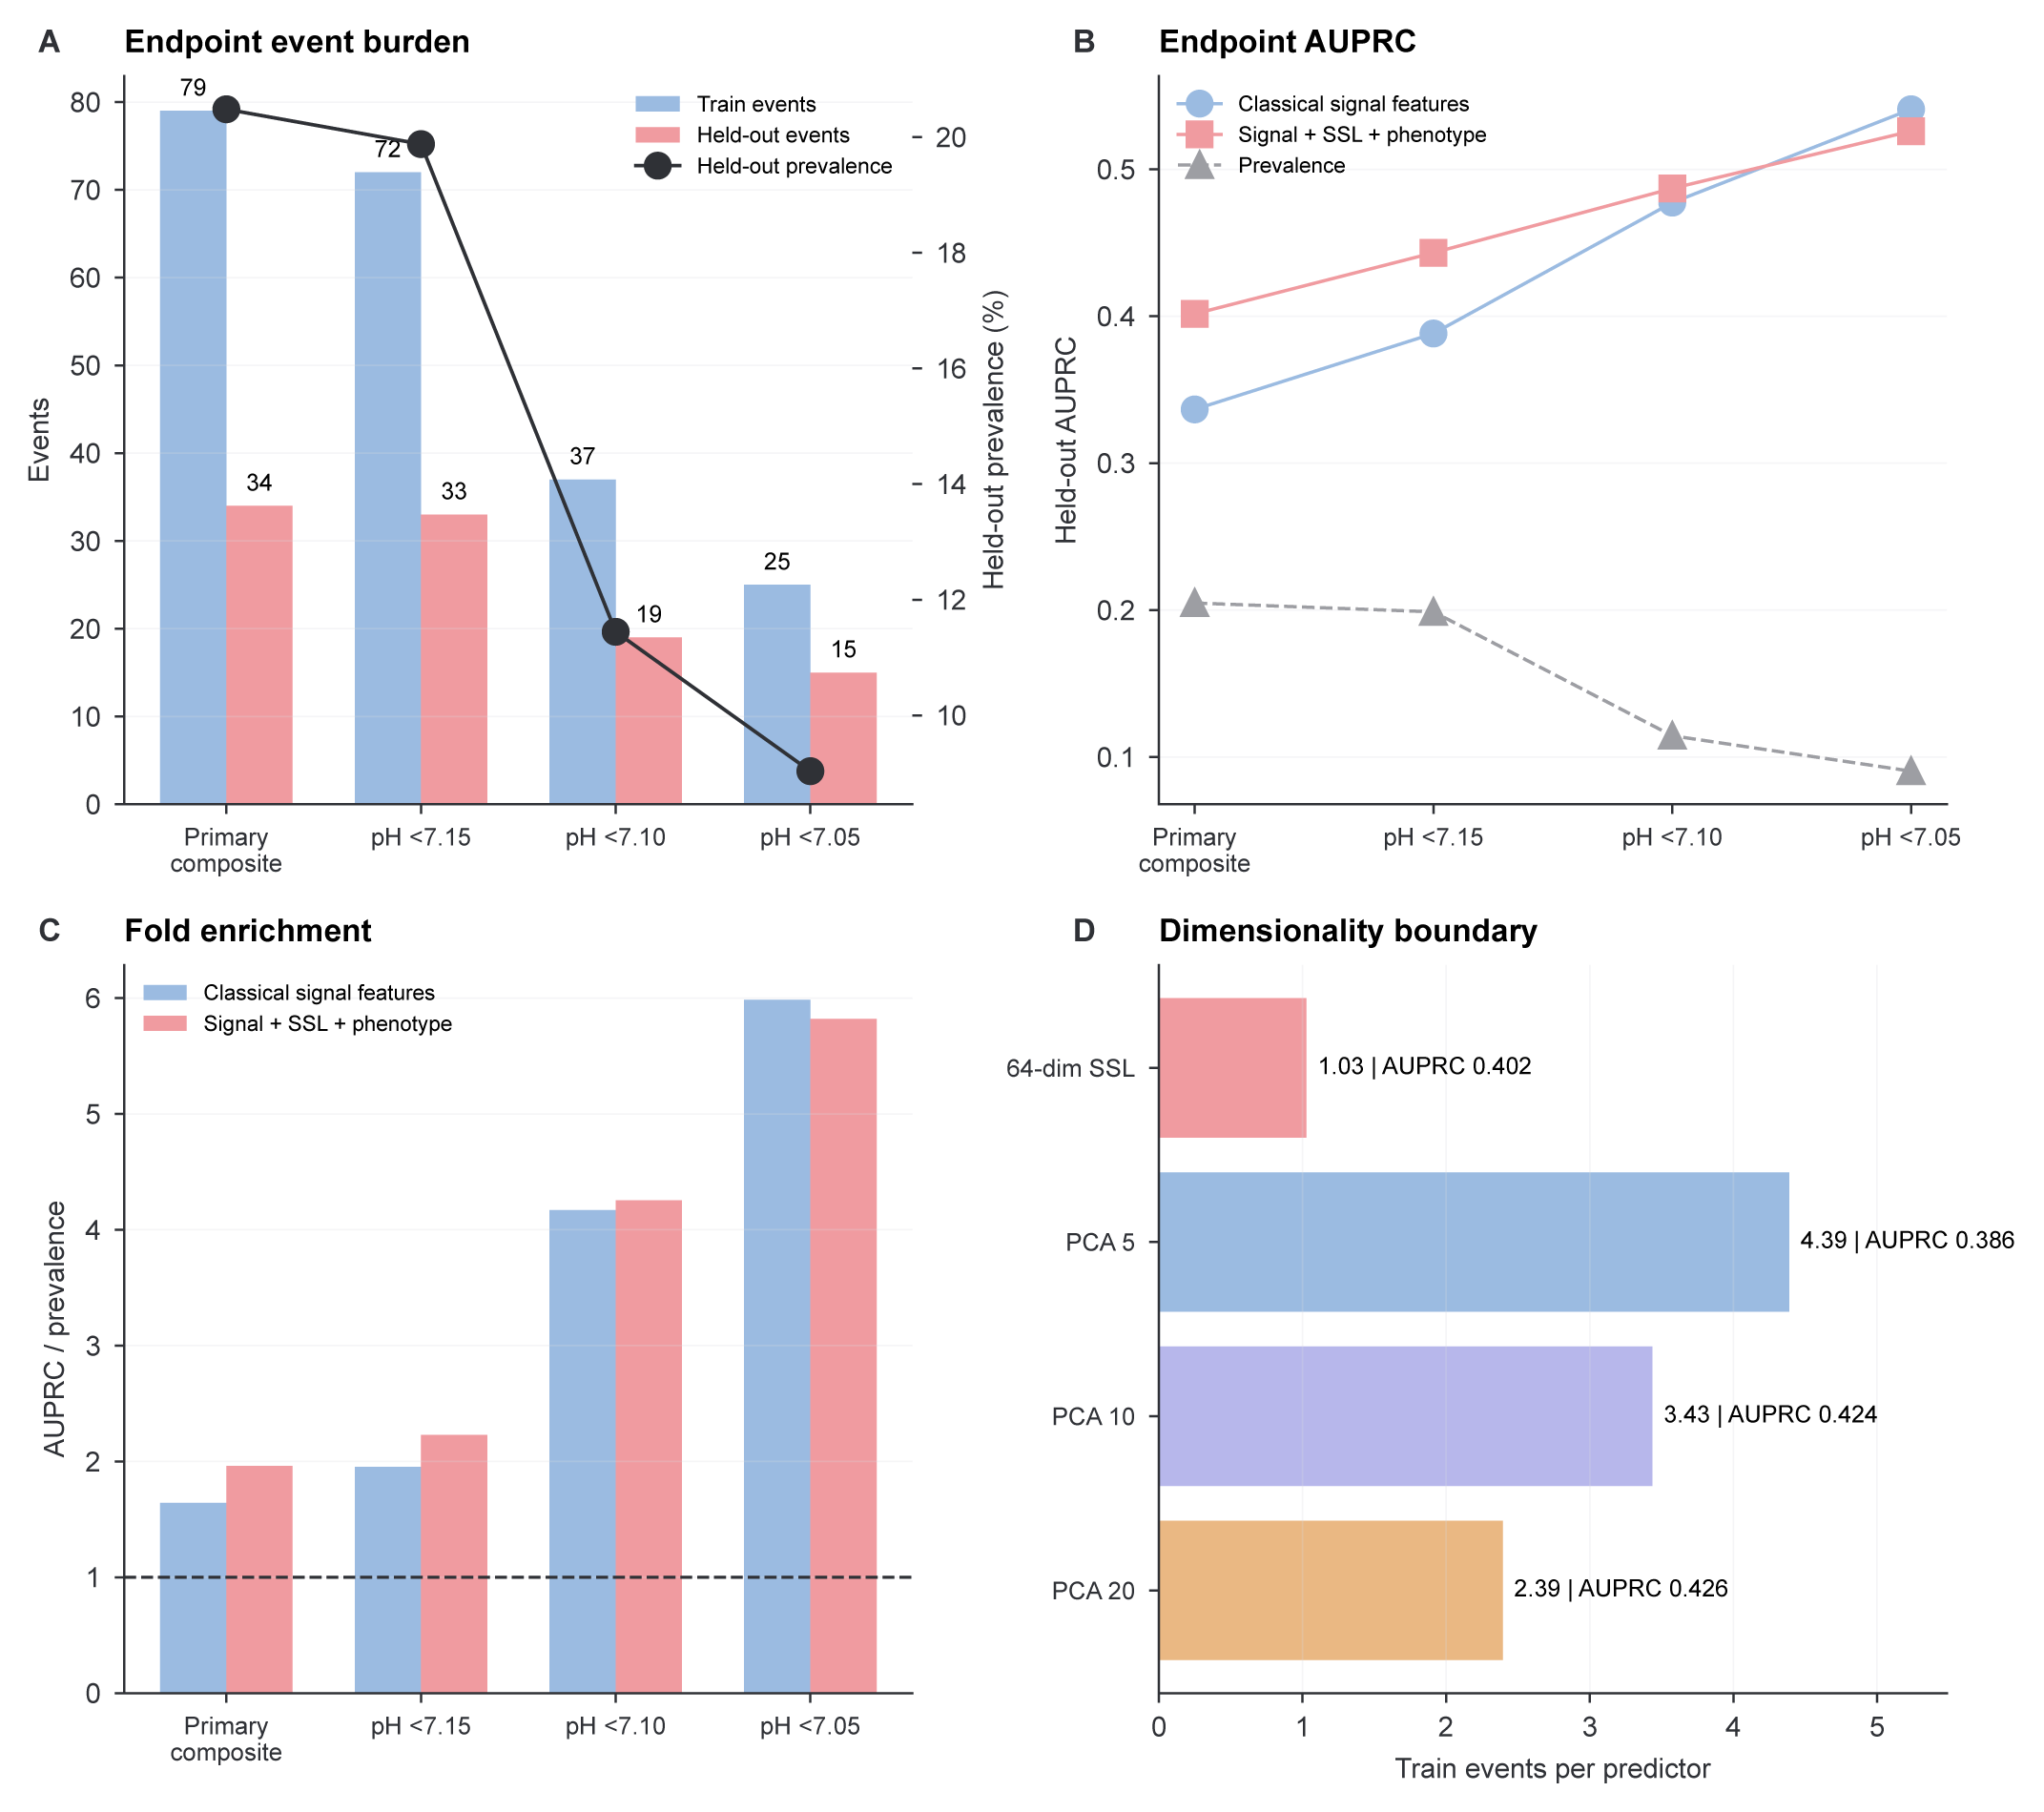
\includegraphics[width=\textwidth]{figures/Supplementary_Figure_S3_endpoint_threshold_and_sample_size.png}
\end{center}
\caption{\textbf{Endpoint-threshold and sample-size sensitivity analyses.} Internal sensitivity analyses for endpoint definition and labelled-sample constraints. (A) Train and held-out event counts with held-out prevalence for the primary pH $<$7.15/Apgar composite and pH-only thresholds. (B) Held-out AUPRC across endpoint definitions for classical signal features and the final signal-plus-SSL-plus-signal-phenotype model, with endpoint prevalence shown as the random-classifier reference. (C) Fold enrichment over endpoint prevalence. (D) Train-event-per-predictor sensitivity for the full 64-dimensional SSL representation and PCA-compressed SSL summaries. These panels are internal sensitivity analyses and do not constitute external outcome validation or a severe-acidemia primary claim.}\label{fig:endpoint_sample_size}
\end{figure}

\clearpage
\section*{Supplementary Tables}
\clearpage

\subsection*{Supplementary Table 1. Dataset sources, cohort scale, record-level split, window counts, and external assessment role}

Complete source table: Supplementary\_\allowbreak{}Table\_\allowbreak{}1\_\allowbreak{}datasets\_\allowbreak{}and\_\allowbreak{}cohort\_\allowbreak{}scale.\allowbreak{}csv. Rows: 8; columns: 10. The display is split into source-defined sub-tables and column blocks to preserve a readable table layout; no non-empty source rows or columns are omitted.

\begin{landscape}
\scriptsize
\setlength\LTleft{0.025\linewidth}
\setlength\LTright{0.025\linewidth}
\setlength{\tabcolsep}{2pt}
\renewcommand{\arraystretch}{1.16}
\begin{longtable}{L{0.184\linewidth} L{0.184\linewidth} L{0.184\linewidth} L{0.184\linewidth} L{0.184\linewidth}}
\caption{Supplementary Table 1, column block 1 of 3}\label{tab:s1_g1_block1}\\
\toprule
dataset or subset & role & records & windows & neonatal risk rate \\
\midrule
\endfirsthead
\multicolumn{5}{l}{\textit{Continued from Supplementary Table 1, column block 1 of 3.}}\\
\toprule
dataset or subset & role & records & windows & neonatal risk rate \\
\midrule
\endhead
\endfoot
\bottomrule
\endlastfoot
CTU-\allowbreak{}UHB complete cohort & primary raw CTG cohort & 552 & 7602 & 0.\allowbreak{}2047 \\
CTU-\allowbreak{}UHB training split & model development & 386 & 5301 & 0.\allowbreak{}2047 \\
CTU-\allowbreak{}UHB held-\allowbreak{}out test split & internal validation & 166 & 2301 & 0.\allowbreak{}2048 \\
CTGDL-\allowbreak{}FHRMA & external representation/\allowbreak{}domain-\allowbreak{}shift assessment & 135 & 2604 &  \\
CTU-\allowbreak{}UHB /\allowbreak{} CTU-\allowbreak{}CHB Intrapartum CTG Database & primary raw signal cohort &  &  &  \\
UCI Cardiotocography & feature-\allowbreak{}level baseline &  &  &  \\
CTGDL & multi-\allowbreak{}source external/\allowbreak{}harmonized resource &  &  &  \\
CTU-\allowbreak{}CHB annotation dataset & optional expert annotation layer &  &  &  \\
\end{longtable}
\normalsize
\end{landscape}


\begin{landscape}
\scriptsize
\setlength\LTleft{0.025\linewidth}
\setlength\LTright{0.025\linewidth}
\setlength{\tabcolsep}{2pt}
\renewcommand{\arraystretch}{1.16}
\begin{longtable}{L{0.184\linewidth} L{0.184\linewidth} L{0.184\linewidth} L{0.184\linewidth} L{0.184\linewidth}}
\caption{Supplementary Table 1, column block 2 of 3}\label{tab:s1_g1_block2}\\
\toprule
dataset or subset & role & notes & url & access \\
\midrule
\endfirsthead
\multicolumn{5}{l}{\textit{Continued from Supplementary Table 1, column block 2 of 3.}}\\
\toprule
dataset or subset & role & notes & url & access \\
\midrule
\endhead
\endfoot
\bottomrule
\endlastfoot
CTU-\allowbreak{}UHB complete cohort & primary raw CTG cohort & Open intrapartum FHR and uterine contraction signals with clinical metadata.\allowbreak{} &  &  \\
CTU-\allowbreak{}UHB training split & model development & Record-\allowbreak{}level split to avoid window leakage.\allowbreak{} &  &  \\
CTU-\allowbreak{}UHB held-\allowbreak{}out test split & internal validation & Held-\allowbreak{}out record-\allowbreak{}level test set for manuscript metrics.\allowbreak{} &  &  \\
CTGDL-\allowbreak{}FHRMA & external representation/\allowbreak{}domain-\allowbreak{}shift assessment & Used for embedding transport and phenotype assignment, not external outcome validation.\allowbreak{} &  &  \\
CTU-\allowbreak{}UHB /\allowbreak{} CTU-\allowbreak{}CHB Intrapartum CTG Database & primary raw signal cohort & 552 intrapartum CTG records with FHR/\allowbreak{}UC signals and clinical metadata & https:\allowbreak{}/\allowbreak{}/\allowbreak{}physionet.\allowbreak{}org/\allowbreak{}content/\allowbreak{}ctu-\allowbreak{}uhb-\allowbreak{}ctgdb/\allowbreak{}1.\allowbreak{}0.\allowbreak{}0/\allowbreak{} & open access \\
UCI Cardiotocography & feature-\allowbreak{}level baseline & 2126 CTG feature rows;\allowbreak{} no raw signal & https:\allowbreak{}/\allowbreak{}/\allowbreak{}archive-\allowbreak{}beta.\allowbreak{}ics.\allowbreak{}uci.\allowbreak{}edu/\allowbreak{}dataset/\allowbreak{}193/\allowbreak{}cardiotocography & open access \\
CTGDL & multi-\allowbreak{}source external/\allowbreak{}harmonized resource & Includes CTU-\allowbreak{}UHB derived files and other sources;\allowbreak{} SPAM subset notes DUA requirement & https:\allowbreak{}/\allowbreak{}/\allowbreak{}zenodo.\allowbreak{}org/\allowbreak{}records/\allowbreak{}18023488 & open record with subset-\allowbreak{}specific caveats \\
CTU-\allowbreak{}CHB annotation dataset & optional expert annotation layer & Useful for clinically interpretable event annotation if files are accessible & https:\allowbreak{}/\allowbreak{}/\allowbreak{}doi.\allowbreak{}org/\allowbreak{}10.\allowbreak{}1016/\allowbreak{}j.\allowbreak{}dib.\allowbreak{}2020.\allowbreak{}105690 & article/\allowbreak{}open supplementary source \\
\end{longtable}
\normalsize
\end{landscape}


\begin{landscape}
\scriptsize
\setlength\LTleft{0.025\linewidth}
\setlength\LTright{0.025\linewidth}
\setlength{\tabcolsep}{2pt}
\renewcommand{\arraystretch}{1.16}
\begin{longtable}{L{0.225\linewidth} L{0.225\linewidth} L{0.225\linewidth} L{0.225\linewidth}}
\caption{Supplementary Table 1, column block 3 of 3}\label{tab:s1_g1_block3}\\
\toprule
dataset or subset & role & license or terms & status \\
\midrule
\endfirsthead
\multicolumn{4}{l}{\textit{Continued from Supplementary Table 1, column block 3 of 3.}}\\
\toprule
dataset or subset & role & license or terms & status \\
\midrule
\endhead
\endfoot
\bottomrule
\endlastfoot
CTU-\allowbreak{}UHB complete cohort & primary raw CTG cohort &  &  \\
CTU-\allowbreak{}UHB training split & model development &  &  \\
CTU-\allowbreak{}UHB held-\allowbreak{}out test split & internal validation &  &  \\
CTGDL-\allowbreak{}FHRMA & external representation/\allowbreak{}domain-\allowbreak{}shift assessment &  &  \\
CTU-\allowbreak{}UHB /\allowbreak{} CTU-\allowbreak{}CHB Intrapartum CTG Database & primary raw signal cohort & Open Data Commons Attribution License v1.\allowbreak{}0 & verified \\
UCI Cardiotocography & feature-\allowbreak{}level baseline & UCI repository terms & verified \\
CTGDL & multi-\allowbreak{}source external/\allowbreak{}harmonized resource & mixed;\allowbreak{} check each subset & verified with caveats \\
CTU-\allowbreak{}CHB annotation dataset & optional expert annotation layer & check publisher/\allowbreak{}data terms & identified \\
\end{longtable}
\normalsize
\end{landscape}


\clearpage

\subsection*{Supplementary Table 2. Held-out model performance with 2000-bootstrap confidence intervals}

Complete source table: Supplementary\_\allowbreak{}Table\_\allowbreak{}2\_\allowbreak{}model\_\allowbreak{}performance\_\allowbreak{}bootstrap.\allowbreak{}csv. Rows: 40; columns: 8. The display is split into source-defined sub-tables and column blocks to preserve a readable table layout; no non-empty source rows or columns are omitted.

\begin{landscape}
\scriptsize
\setlength\LTleft{0.025\linewidth}
\setlength\LTright{0.025\linewidth}
\setlength{\tabcolsep}{2pt}
\renewcommand{\arraystretch}{1.16}
\begin{longtable}{L{0.184\linewidth} L{0.184\linewidth} L{0.184\linewidth} L{0.184\linewidth} L{0.184\linewidth}}
\caption{Supplementary Table 2, column block 1 of 2}\label{tab:s2_g1_block1}\\
\toprule
model & model label & metric & point & bootstrap mean \\
\midrule
\endfirsthead
\multicolumn{5}{l}{\textit{Continued from Supplementary Table 2, column block 1 of 2.}}\\
\toprule
model & model label & metric & point & bootstrap mean \\
\midrule
\endhead
\endfoot
\bottomrule
\endlastfoot
Classical signal features & Signal features & auroc & 0.\allowbreak{}6303 & 0.\allowbreak{}6293 \\
Classical signal features & Signal features & auprc & 0.\allowbreak{}3366 & 0.\allowbreak{}3522 \\
Classical signal features & Signal features & brier & 0.\allowbreak{}2525 & 0.\allowbreak{}2528 \\
Classical signal features & Signal features & Calibration intercept & -\allowbreak{}1.\allowbreak{}384 &  \\
Classical signal features & Signal features & Calibration slope & 0.\allowbreak{}4876 &  \\
SSL embeddings & SSL embeddings & auroc & 0.\allowbreak{}4947 & 0.\allowbreak{}4936 \\
SSL embeddings & SSL embeddings & auprc & 0.\allowbreak{}2125 & 0.\allowbreak{}2269 \\
SSL embeddings & SSL embeddings & brier & 0.\allowbreak{}2639 & 0.\allowbreak{}2639 \\
SSL embeddings & SSL embeddings & Calibration intercept & -\allowbreak{}1.\allowbreak{}361 &  \\
SSL embeddings & SSL embeddings & Calibration slope & -\allowbreak{}0.\allowbreak{}0415 &  \\
Signal + SSL & Signal + SSL & auroc & 0.\allowbreak{}6025 & 0.\allowbreak{}6007 \\
Signal + SSL & Signal + SSL & auprc & 0.\allowbreak{}3765 & 0.\allowbreak{}3832 \\
Signal + SSL & Signal + SSL & brier & 0.\allowbreak{}2701 & 0.\allowbreak{}2707 \\
Signal + SSL & Signal + SSL & Calibration intercept & -\allowbreak{}1.\allowbreak{}36 &  \\
Signal + SSL & Signal + SSL & Calibration slope & 0.\allowbreak{}3136 &  \\
signal phenotype only & Signal phenotype only & auroc & 0.\allowbreak{}6003 & 0.\allowbreak{}6 \\
signal phenotype only & Signal phenotype only & auprc & 0.\allowbreak{}2488 & 0.\allowbreak{}2538 \\
signal phenotype only & Signal phenotype only & brier & 0.\allowbreak{}2523 & 0.\allowbreak{}2525 \\
signal phenotype only & Signal phenotype only & Calibration intercept & -\allowbreak{}1.\allowbreak{}368 &  \\
signal phenotype only & Signal phenotype only & Calibration slope & 0.\allowbreak{}4662 &  \\
SSL phenotype only & SSL phenotype only & auroc & 0.\allowbreak{}5949 & 0.\allowbreak{}5962 \\
SSL phenotype only & SSL phenotype only & auprc & 0.\allowbreak{}246 & 0.\allowbreak{}2543 \\
SSL phenotype only & SSL phenotype only & brier & 0.\allowbreak{}246 & 0.\allowbreak{}2458 \\
SSL phenotype only & SSL phenotype only & Calibration intercept & -\allowbreak{}1.\allowbreak{}38 &  \\
SSL phenotype only & SSL phenotype only & Calibration slope & 1.\allowbreak{}456 &  \\
signal + signal phenotype & Signal + signal phenotype & auroc & 0.\allowbreak{}6328 & 0.\allowbreak{}6321 \\
signal + signal phenotype & Signal + signal phenotype & auprc & 0.\allowbreak{}3495 & 0.\allowbreak{}3618 \\
signal + signal phenotype & Signal + signal phenotype & brier & 0.\allowbreak{}2503 & 0.\allowbreak{}2506 \\
signal + signal phenotype & Signal + signal phenotype & Calibration intercept & -\allowbreak{}1.\allowbreak{}377 &  \\
signal + signal phenotype & Signal + signal phenotype & Calibration slope & 0.\allowbreak{}5031 &  \\
Signal + SSL phenotype & Signal + SSL phenotype & auroc & 0.\allowbreak{}6667 & 0.\allowbreak{}6654 \\
Signal + SSL phenotype & Signal + SSL phenotype & auprc & 0.\allowbreak{}3732 & 0.\allowbreak{}3879 \\
Signal + SSL phenotype & Signal + SSL phenotype & brier & 0.\allowbreak{}2483 & 0.\allowbreak{}2486 \\
Signal + SSL phenotype & Signal + SSL phenotype & Calibration intercept & -\allowbreak{}1.\allowbreak{}426 &  \\
Signal + SSL phenotype & Signal + SSL phenotype & Calibration slope & 0.\allowbreak{}5602 &  \\
Signal + SSL + phenotype & Signal + SSL + signal phenotype & auroc & 0.\allowbreak{}6168 & 0.\allowbreak{}6151 \\
Signal + SSL + phenotype & Signal + SSL + signal phenotype & auprc & 0.\allowbreak{}4016 & 0.\allowbreak{}4069 \\
Signal + SSL + phenotype & Signal + SSL + signal phenotype & brier & 0.\allowbreak{}2652 & 0.\allowbreak{}2657 \\
Signal + SSL + phenotype & Signal + SSL + signal phenotype & Calibration intercept & -\allowbreak{}1.\allowbreak{}359 &  \\
Signal + SSL + phenotype & Signal + SSL + signal phenotype & Calibration slope & 0.\allowbreak{}3448 &  \\
\end{longtable}
\normalsize
\end{landscape}


\begin{landscape}
\scriptsize
\setlength\LTleft{0.025\linewidth}
\setlength\LTright{0.025\linewidth}
\setlength{\tabcolsep}{2pt}
\renewcommand{\arraystretch}{1.16}
\begin{longtable}{L{0.184\linewidth} L{0.184\linewidth} L{0.184\linewidth} L{0.184\linewidth} L{0.184\linewidth}}
\caption{Supplementary Table 2, column block 2 of 2}\label{tab:s2_g1_block2}\\
\toprule
model & model label & 95\% CI lower & 95\% CI upper & Valid bootstrap resamples \\
\midrule
\endfirsthead
\multicolumn{5}{l}{\textit{Continued from Supplementary Table 2, column block 2 of 2.}}\\
\toprule
model & model label & 95\% CI lower & 95\% CI upper & Valid bootstrap resamples \\
\midrule
\endhead
\endfoot
\bottomrule
\endlastfoot
Classical signal features & Signal features & 0.\allowbreak{}5254 & 0.\allowbreak{}7284 & 2000 \\
Classical signal features & Signal features & 0.\allowbreak{}2173 & 0.\allowbreak{}4941 & 2000 \\
Classical signal features & Signal features & 0.\allowbreak{}2234 & 0.\allowbreak{}2834 & 2000 \\
Classical signal features & Signal features &  &  &  \\
Classical signal features & Signal features &  &  &  \\
SSL embeddings & SSL embeddings & 0.\allowbreak{}3795 & 0.\allowbreak{}6035 & 2000 \\
SSL embeddings & SSL embeddings & 0.\allowbreak{}1477 & 0.\allowbreak{}3248 & 2000 \\
SSL embeddings & SSL embeddings & 0.\allowbreak{}2394 & 0.\allowbreak{}29 & 2000 \\
SSL embeddings & SSL embeddings &  &  &  \\
SSL embeddings & SSL embeddings &  &  &  \\
Signal + SSL & Signal + SSL & 0.\allowbreak{}4927 & 0.\allowbreak{}7045 & 2000 \\
Signal + SSL & Signal + SSL & 0.\allowbreak{}2399 & 0.\allowbreak{}5243 & 2000 \\
Signal + SSL & Signal + SSL & 0.\allowbreak{}2315 & 0.\allowbreak{}3066 & 2000 \\
Signal + SSL & Signal + SSL &  &  &  \\
Signal + SSL & Signal + SSL &  &  &  \\
signal phenotype only & Signal phenotype only & 0.\allowbreak{}4951 & 0.\allowbreak{}697 & 2000 \\
signal phenotype only & Signal phenotype only & 0.\allowbreak{}168 & 0.\allowbreak{}3519 & 2000 \\
signal phenotype only & Signal phenotype only & 0.\allowbreak{}2298 & 0.\allowbreak{}2751 & 2000 \\
signal phenotype only & Signal phenotype only &  &  &  \\
signal phenotype only & Signal phenotype only &  &  &  \\
SSL phenotype only & SSL phenotype only & 0.\allowbreak{}4917 & 0.\allowbreak{}6912 & 2000 \\
SSL phenotype only & SSL phenotype only & 0.\allowbreak{}1654 & 0.\allowbreak{}3538 & 2000 \\
SSL phenotype only & SSL phenotype only & 0.\allowbreak{}2368 & 0.\allowbreak{}2548 & 2000 \\
SSL phenotype only & SSL phenotype only &  &  &  \\
SSL phenotype only & SSL phenotype only &  &  &  \\
signal + signal phenotype & Signal + signal phenotype & 0.\allowbreak{}5243 & 0.\allowbreak{}7306 & 2000 \\
signal + signal phenotype & Signal + signal phenotype & 0.\allowbreak{}221 & 0.\allowbreak{}5007 & 2000 \\
signal + signal phenotype & Signal + signal phenotype & 0.\allowbreak{}2216 & 0.\allowbreak{}2807 & 2000 \\
signal + signal phenotype & Signal + signal phenotype &  &  &  \\
signal + signal phenotype & Signal + signal phenotype &  &  &  \\
Signal + SSL phenotype & Signal + SSL phenotype & 0.\allowbreak{}5642 & 0.\allowbreak{}7578 & 2000 \\
Signal + SSL phenotype & Signal + SSL phenotype & 0.\allowbreak{}246 & 0.\allowbreak{}5381 & 2000 \\
Signal + SSL phenotype & Signal + SSL phenotype & 0.\allowbreak{}2189 & 0.\allowbreak{}2814 & 2000 \\
Signal + SSL phenotype & Signal + SSL phenotype &  &  &  \\
Signal + SSL phenotype & Signal + SSL phenotype &  &  &  \\
Signal + SSL + phenotype & Signal + SSL + signal phenotype & 0.\allowbreak{}5111 & 0.\allowbreak{}7191 & 2000 \\
Signal + SSL + phenotype & Signal + SSL + signal phenotype & 0.\allowbreak{}2605 & 0.\allowbreak{}5471 & 2000 \\
Signal + SSL + phenotype & Signal + SSL + signal phenotype & 0.\allowbreak{}226 & 0.\allowbreak{}302 & 2000 \\
Signal + SSL + phenotype & Signal + SSL + signal phenotype &  &  &  \\
Signal + SSL + phenotype & Signal + SSL + signal phenotype &  &  &  \\
\end{longtable}
\normalsize
\end{landscape}


\clearpage

\subsection*{Supplementary Table 3. Bootstrap pairwise model differences and zero-crossing flags}

Complete source table: Supplementary\_\allowbreak{}Table\_\allowbreak{}3\_\allowbreak{}bootstrap\_\allowbreak{}model\_\allowbreak{}differences.\allowbreak{}csv. Rows: 9; columns: 7. The display is split into source-defined sub-tables and column blocks to preserve a readable table layout; no non-empty source rows or columns are omitted.

\begin{landscape}
\scriptsize
\setlength\LTleft{0.025\linewidth}
\setlength\LTright{0.025\linewidth}
\setlength{\tabcolsep}{2pt}
\renewcommand{\arraystretch}{1.16}
\begin{longtable}{L{0.184\linewidth} L{0.184\linewidth} L{0.184\linewidth} L{0.184\linewidth} L{0.184\linewidth}}
\caption{Supplementary Table 3, column block 1 of 2}\label{tab:s3_g1_block1}\\
\toprule
comparison & metric & bootstrap mean difference & 95\% CI lower & 95\% CI upper \\
\midrule
\endfirsthead
\multicolumn{5}{l}{\textit{Continued from Supplementary Table 3, column block 1 of 2.}}\\
\toprule
comparison & metric & bootstrap mean difference & 95\% CI lower & 95\% CI upper \\
\midrule
\endhead
\endfoot
\bottomrule
\endlastfoot
Signal + SSL minus Classical signal features & auroc & -\allowbreak{}0.\allowbreak{}0286 & -\allowbreak{}0.\allowbreak{}1153 & 0.\allowbreak{}0541 \\
Signal + SSL minus Classical signal features & auprc & 0.\allowbreak{}031 & -\allowbreak{}0.\allowbreak{}0527 & 0.\allowbreak{}1077 \\
Signal + SSL minus Classical signal features & brier & 0.\allowbreak{}0179 & -\allowbreak{}0.\allowbreak{}0067 & 0.\allowbreak{}0434 \\
Signal + SSL + phenotype minus Classical signal features & auroc & -\allowbreak{}0.\allowbreak{}0142 & -\allowbreak{}0.\allowbreak{}1012 & 0.\allowbreak{}0679 \\
Signal + SSL + phenotype minus Classical signal features & auprc & 0.\allowbreak{}0548 & -\allowbreak{}0.\allowbreak{}0354 & 0.\allowbreak{}1519 \\
Signal + SSL + phenotype minus Classical signal features & brier & 0.\allowbreak{}013 & -\allowbreak{}0.\allowbreak{}0129 & 0.\allowbreak{}0386 \\
Signal + SSL minus signal + signal phenotype & auroc & -\allowbreak{}0.\allowbreak{}0313 & -\allowbreak{}0.\allowbreak{}114 & 0.\allowbreak{}0509 \\
Signal + SSL minus signal + signal phenotype & auprc & 0.\allowbreak{}0213 & -\allowbreak{}0.\allowbreak{}0613 & 0.\allowbreak{}1056 \\
Signal + SSL minus signal + signal phenotype & brier & 0.\allowbreak{}0201 & -\allowbreak{}0.\allowbreak{}0046 & 0.\allowbreak{}0447 \\
\end{longtable}
\normalsize
\end{landscape}


\begin{landscape}
\scriptsize
\setlength\LTleft{0.025\linewidth}
\setlength\LTright{0.025\linewidth}
\setlength{\tabcolsep}{2pt}
\renewcommand{\arraystretch}{1.16}
\begin{longtable}{L{0.225\linewidth} L{0.225\linewidth} L{0.225\linewidth} L{0.225\linewidth}}
\caption{Supplementary Table 3, column block 2 of 2}\label{tab:s3_g1_block2}\\
\toprule
comparison & metric & Valid bootstrap resamples & CI excludes zero \\
\midrule
\endfirsthead
\multicolumn{4}{l}{\textit{Continued from Supplementary Table 3, column block 2 of 2.}}\\
\toprule
comparison & metric & Valid bootstrap resamples & CI excludes zero \\
\midrule
\endhead
\endfoot
\bottomrule
\endlastfoot
Signal + SSL minus Classical signal features & auroc & 2000 & False \\
Signal + SSL minus Classical signal features & auprc & 2000 & False \\
Signal + SSL minus Classical signal features & brier & 2000 & False \\
Signal + SSL + phenotype minus Classical signal features & auroc & 2000 & False \\
Signal + SSL + phenotype minus Classical signal features & auprc & 2000 & False \\
Signal + SSL + phenotype minus Classical signal features & brier & 2000 & False \\
Signal + SSL minus signal + signal phenotype & auroc & 2000 & False \\
Signal + SSL minus signal + signal phenotype & auprc & 2000 & False \\
Signal + SSL minus signal + signal phenotype & brier & 2000 & False \\
\end{longtable}
\normalsize
\end{landscape}


\clearpage

\subsection*{Supplementary Table 4. Signal and SSL phenotype summaries with representative prototype records}

Complete source table: Supplementary\_\allowbreak{}Table\_\allowbreak{}4\_\allowbreak{}dynamic\_\allowbreak{}phenotype\_\allowbreak{}summary\_\allowbreak{}and\_\allowbreak{}prototypes.\allowbreak{}csv. Rows: 8; columns: 39. The display is split into source-defined sub-tables and column blocks to preserve a readable table layout; no non-empty source rows or columns are omitted.

\subsubsection*{phenotype type: signal phenotype}

\begin{landscape}
\scriptsize
\setlength\LTleft{0.025\linewidth}
\setlength\LTright{0.025\linewidth}
\setlength{\tabcolsep}{2pt}
\renewcommand{\arraystretch}{1.16}
\begin{longtable}{L{0.184\linewidth} L{0.184\linewidth} L{0.184\linewidth} L{0.184\linewidth} L{0.184\linewidth}}
\caption{Supplementary Table 4, signal phenotype, column block 1 of 12}\label{tab:s4_g1_block1}\\
\toprule
phenotype & neonatal risk count & neonatal risk mean & neonatal risk median & cord ph count \\
\midrule
\endfirsthead
\multicolumn{5}{l}{\textit{Continued from Supplementary Table 4, signal phenotype, column block 1 of 12.}}\\
\toprule
phenotype & neonatal risk count & neonatal risk mean & neonatal risk median & cord ph count \\
\midrule
\endhead
\endfoot
\bottomrule
\endlastfoot
1 & 160 & 0.\allowbreak{}1438 & 0 & 160 \\
2 & 157 & 0.\allowbreak{}3439 & 0 & 157 \\
3 & 130 & 0.\allowbreak{}1923 & 0 & 130 \\
4 & 105 & 0.\allowbreak{}1048 & 0 & 105 \\
\end{longtable}
\normalsize
\end{landscape}


\begin{landscape}
\scriptsize
\setlength\LTleft{0.025\linewidth}
\setlength\LTright{0.025\linewidth}
\setlength{\tabcolsep}{2pt}
\renewcommand{\arraystretch}{1.16}
\begin{longtable}{L{0.184\linewidth} L{0.184\linewidth} L{0.184\linewidth} L{0.184\linewidth} L{0.184\linewidth}}
\caption{Supplementary Table 4, signal phenotype, column block 2 of 12}\label{tab:s4_g1_block2}\\
\toprule
phenotype & neonatal risk count & cord ph mean & cord ph median & apgar5 count \\
\midrule
\endfirsthead
\multicolumn{5}{l}{\textit{Continued from Supplementary Table 4, signal phenotype, column block 2 of 12.}}\\
\toprule
phenotype & neonatal risk count & cord ph mean & cord ph median & apgar5 count \\
\midrule
\endhead
\endfoot
\bottomrule
\endlastfoot
1 & 160 & 7.\allowbreak{}254 & 7.\allowbreak{}27 & 160 \\
2 & 157 & 7.\allowbreak{}188 & 7.\allowbreak{}2 & 157 \\
3 & 130 & 7.\allowbreak{}236 & 7.\allowbreak{}25 & 130 \\
4 & 105 & 7.\allowbreak{}25 & 7.\allowbreak{}25 & 105 \\
\end{longtable}
\normalsize
\end{landscape}


\begin{landscape}
\scriptsize
\setlength\LTleft{0.025\linewidth}
\setlength\LTright{0.025\linewidth}
\setlength{\tabcolsep}{2pt}
\renewcommand{\arraystretch}{1.16}
\begin{longtable}{L{0.184\linewidth} L{0.184\linewidth} L{0.184\linewidth} L{0.184\linewidth} L{0.184\linewidth}}
\caption{Supplementary Table 4, signal phenotype, column block 3 of 12}\label{tab:s4_g1_block3}\\
\toprule
phenotype & neonatal risk count & apgar5 mean & apgar5 median & FHR mean count \\
\midrule
\endfirsthead
\multicolumn{5}{l}{\textit{Continued from Supplementary Table 4, signal phenotype, column block 3 of 12.}}\\
\toprule
phenotype & neonatal risk count & apgar5 mean & apgar5 median & FHR mean count \\
\midrule
\endhead
\endfoot
\bottomrule
\endlastfoot
1 & 160 & 9.\allowbreak{}219 & 9 & 160 \\
2 & 157 & 8.\allowbreak{}783 & 9 & 157 \\
3 & 130 & 9.\allowbreak{}077 & 9 & 130 \\
4 & 105 & 9.\allowbreak{}257 & 9 & 105 \\
\end{longtable}
\normalsize
\end{landscape}


\begin{landscape}
\scriptsize
\setlength\LTleft{0.025\linewidth}
\setlength\LTright{0.025\linewidth}
\setlength{\tabcolsep}{2pt}
\renewcommand{\arraystretch}{1.16}
\begin{longtable}{L{0.184\linewidth} L{0.184\linewidth} L{0.184\linewidth} L{0.184\linewidth} L{0.184\linewidth}}
\caption{Supplementary Table 4, signal phenotype, column block 4 of 12}\label{tab:s4_g1_block4}\\
\toprule
phenotype & neonatal risk count & FHR mean mean & FHR mean median & FHR sd count \\
\midrule
\endfirsthead
\multicolumn{5}{l}{\textit{Continued from Supplementary Table 4, signal phenotype, column block 4 of 12.}}\\
\toprule
phenotype & neonatal risk count & FHR mean mean & FHR mean median & FHR sd count \\
\midrule
\endhead
\endfoot
\bottomrule
\endlastfoot
1 & 160 & 125.\allowbreak{}1 & 125.\allowbreak{}5 & 160 \\
2 & 157 & 134.\allowbreak{}6 & 134.\allowbreak{}9 & 157 \\
3 & 130 & 148.\allowbreak{}4 & 146.\allowbreak{}3 & 130 \\
4 & 105 & 132.\allowbreak{}7 & 133.\allowbreak{}8 & 105 \\
\end{longtable}
\normalsize
\end{landscape}


\begin{landscape}
\scriptsize
\setlength\LTleft{0.025\linewidth}
\setlength\LTright{0.025\linewidth}
\setlength{\tabcolsep}{2pt}
\renewcommand{\arraystretch}{1.16}
\begin{longtable}{L{0.184\linewidth} L{0.184\linewidth} L{0.184\linewidth} L{0.184\linewidth} L{0.184\linewidth}}
\caption{Supplementary Table 4, signal phenotype, column block 5 of 12}\label{tab:s4_g1_block5}\\
\toprule
phenotype & neonatal risk count & FHR sd mean & FHR sd median & FHR p05 count \\
\midrule
\endfirsthead
\multicolumn{5}{l}{\textit{Continued from Supplementary Table 4, signal phenotype, column block 5 of 12.}}\\
\toprule
phenotype & neonatal risk count & FHR sd mean & FHR sd median & FHR p05 count \\
\midrule
\endhead
\endfoot
\bottomrule
\endlastfoot
1 & 160 & 15.\allowbreak{}25 & 15.\allowbreak{}51 & 160 \\
2 & 157 & 22.\allowbreak{}22 & 21.\allowbreak{}92 & 157 \\
3 & 130 & 14.\allowbreak{}33 & 14.\allowbreak{}26 & 130 \\
4 & 105 & 15.\allowbreak{}03 & 15.\allowbreak{}13 & 105 \\
\end{longtable}
\normalsize
\end{landscape}


\begin{landscape}
\scriptsize
\setlength\LTleft{0.025\linewidth}
\setlength\LTright{0.025\linewidth}
\setlength{\tabcolsep}{2pt}
\renewcommand{\arraystretch}{1.16}
\begin{longtable}{L{0.184\linewidth} L{0.184\linewidth} L{0.184\linewidth} L{0.184\linewidth} L{0.184\linewidth}}
\caption{Supplementary Table 4, signal phenotype, column block 6 of 12}\label{tab:s4_g1_block6}\\
\toprule
phenotype & neonatal risk count & FHR p05 mean & FHR p05 median & UC mean count \\
\midrule
\endfirsthead
\multicolumn{5}{l}{\textit{Continued from Supplementary Table 4, signal phenotype, column block 6 of 12.}}\\
\toprule
phenotype & neonatal risk count & FHR p05 mean & FHR p05 median & UC mean count \\
\midrule
\endhead
\endfoot
\bottomrule
\endlastfoot
1 & 160 & 96.\allowbreak{}11 & 96.\allowbreak{}5 & 160 \\
2 & 157 & 88.\allowbreak{}23 & 88.\allowbreak{}5 & 157 \\
3 & 130 & 122.\allowbreak{}6 & 121.\allowbreak{}6 & 130 \\
4 & 105 & 103.\allowbreak{}7 & 104.\allowbreak{}2 & 105 \\
\end{longtable}
\normalsize
\end{landscape}


\begin{landscape}
\scriptsize
\setlength\LTleft{0.025\linewidth}
\setlength\LTright{0.025\linewidth}
\setlength{\tabcolsep}{2pt}
\renewcommand{\arraystretch}{1.16}
\begin{longtable}{L{0.184\linewidth} L{0.184\linewidth} L{0.184\linewidth} L{0.184\linewidth} L{0.184\linewidth}}
\caption{Supplementary Table 4, signal phenotype, column block 7 of 12}\label{tab:s4_g1_block7}\\
\toprule
phenotype & neonatal risk count & UC mean mean & UC mean median & UC p95 count \\
\midrule
\endfirsthead
\multicolumn{5}{l}{\textit{Continued from Supplementary Table 4, signal phenotype, column block 7 of 12.}}\\
\toprule
phenotype & neonatal risk count & UC mean mean & UC mean median & UC p95 count \\
\midrule
\endhead
\endfoot
\bottomrule
\endlastfoot
1 & 160 & 14.\allowbreak{}26 & 14.\allowbreak{}12 & 160 \\
2 & 157 & 20.\allowbreak{}22 & 19.\allowbreak{}12 & 157 \\
3 & 130 & 16.\allowbreak{}45 & 16.\allowbreak{}08 & 130 \\
4 & 105 & 31.\allowbreak{}3 & 29.\allowbreak{}84 & 105 \\
\end{longtable}
\normalsize
\end{landscape}


\begin{landscape}
\scriptsize
\setlength\LTleft{0.025\linewidth}
\setlength\LTright{0.025\linewidth}
\setlength{\tabcolsep}{2pt}
\renewcommand{\arraystretch}{1.16}
\begin{longtable}{L{0.184\linewidth} L{0.184\linewidth} L{0.184\linewidth} L{0.184\linewidth} L{0.184\linewidth}}
\caption{Supplementary Table 4, signal phenotype, column block 8 of 12}\label{tab:s4_g1_block8}\\
\toprule
phenotype & neonatal risk count & UC p95 mean & UC p95 median & FHR UC corr count \\
\midrule
\endfirsthead
\multicolumn{5}{l}{\textit{Continued from Supplementary Table 4, signal phenotype, column block 8 of 12.}}\\
\toprule
phenotype & neonatal risk count & UC p95 mean & UC p95 median & FHR UC corr count \\
\midrule
\endhead
\endfoot
\bottomrule
\endlastfoot
1 & 160 & 40.\allowbreak{}08 & 38.\allowbreak{}5 & 159 \\
2 & 157 & 58.\allowbreak{}02 & 56 & 156 \\
3 & 130 & 47.\allowbreak{}62 & 46 & 130 \\
4 & 105 & 90.\allowbreak{}42 & 92 & 105 \\
\end{longtable}
\normalsize
\end{landscape}


\begin{landscape}
\scriptsize
\setlength\LTleft{0.025\linewidth}
\setlength\LTright{0.025\linewidth}
\setlength{\tabcolsep}{2pt}
\renewcommand{\arraystretch}{1.16}
\begin{longtable}{L{0.184\linewidth} L{0.184\linewidth} L{0.184\linewidth} L{0.184\linewidth} L{0.184\linewidth}}
\caption{Supplementary Table 4, signal phenotype, column block 9 of 12}\label{tab:s4_g1_block9}\\
\toprule
phenotype & neonatal risk count & FHR UC corr mean & FHR UC corr median & deceleration proxy count count \\
\midrule
\endfirsthead
\multicolumn{5}{l}{\textit{Continued from Supplementary Table 4, signal phenotype, column block 9 of 12.}}\\
\toprule
phenotype & neonatal risk count & FHR UC corr mean & FHR UC corr median & deceleration proxy count count \\
\midrule
\endhead
\endfoot
\bottomrule
\endlastfoot
1 & 160 & 0.\allowbreak{}0105 & -\allowbreak{}0.\allowbreak{}0061 & 160 \\
2 & 157 & -\allowbreak{}0.\allowbreak{}0139 & -\allowbreak{}0.\allowbreak{}0237 & 157 \\
3 & 130 & 0.\allowbreak{}0018 & -\allowbreak{}0.\allowbreak{}0146 & 130 \\
4 & 105 & -\allowbreak{}0.\allowbreak{}0821 & -\allowbreak{}0.\allowbreak{}0632 & 105 \\
\end{longtable}
\normalsize
\end{landscape}


\begin{landscape}
\scriptsize
\setlength\LTleft{0.025\linewidth}
\setlength\LTright{0.025\linewidth}
\setlength{\tabcolsep}{2pt}
\renewcommand{\arraystretch}{1.16}
\begin{longtable}{L{0.184\linewidth} L{0.184\linewidth} L{0.184\linewidth} L{0.184\linewidth} L{0.184\linewidth}}
\caption{Supplementary Table 4, signal phenotype, column block 10 of 12}\label{tab:s4_g1_block10}\\
\toprule
phenotype & neonatal risk count & deceleration proxy count mean & deceleration proxy count median & record id \\
\midrule
\endfirsthead
\multicolumn{5}{l}{\textit{Continued from Supplementary Table 4, signal phenotype, column block 10 of 12.}}\\
\toprule
phenotype & neonatal risk count & deceleration proxy count mean & deceleration proxy count median & record id \\
\midrule
\endhead
\endfoot
\bottomrule
\endlastfoot
1 & 160 & 1976.\allowbreak{}3 & 1850 & 1122 \\
2 & 157 & 3530.\allowbreak{}5 & 3404 & 1016 \\
3 & 130 & 1475.\allowbreak{}1 & 1406.\allowbreak{}5 & 1353 \\
4 & 105 & 1894.\allowbreak{}7 & 1905 & 1271 \\
\end{longtable}
\normalsize
\end{landscape}


\begin{landscape}
\scriptsize
\setlength\LTleft{0.025\linewidth}
\setlength\LTright{0.025\linewidth}
\setlength{\tabcolsep}{2pt}
\renewcommand{\arraystretch}{1.16}
\begin{longtable}{L{0.184\linewidth} L{0.184\linewidth} L{0.184\linewidth} L{0.184\linewidth} L{0.184\linewidth}}
\caption{Supplementary Table 4, signal phenotype, column block 11 of 12}\label{tab:s4_g1_block11}\\
\toprule
phenotype & neonatal risk count & distance to centroid & neonatal risk & cord ph \\
\midrule
\endfirsthead
\multicolumn{5}{l}{\textit{Continued from Supplementary Table 4, signal phenotype, column block 11 of 12.}}\\
\toprule
phenotype & neonatal risk count & distance to centroid & neonatal risk & cord ph \\
\midrule
\endhead
\endfoot
\bottomrule
\endlastfoot
1 & 160 & 0.\allowbreak{}6891 & 0 & 7.\allowbreak{}25 \\
2 & 157 & 0.\allowbreak{}5105 & 0 & 7.\allowbreak{}32 \\
3 & 130 & 0.\allowbreak{}405 & 0 & 7.\allowbreak{}2 \\
4 & 105 & 1.\allowbreak{}001 & 0 & 7.\allowbreak{}31 \\
\end{longtable}
\normalsize
\end{landscape}


\begin{landscape}
\scriptsize
\setlength\LTleft{0.025\linewidth}
\setlength\LTright{0.025\linewidth}
\setlength{\tabcolsep}{2pt}
\renewcommand{\arraystretch}{1.16}
\begin{longtable}{L{0.184\linewidth} L{0.184\linewidth} L{0.184\linewidth} L{0.184\linewidth} L{0.184\linewidth}}
\caption{Supplementary Table 4, signal phenotype, column block 12 of 12}\label{tab:s4_g1_block12}\\
\toprule
phenotype & neonatal risk count & apgar5 & n records in phenotype & figure \\
\midrule
\endfirsthead
\multicolumn{5}{l}{\textit{Continued from Supplementary Table 4, signal phenotype, column block 12 of 12.}}\\
\toprule
phenotype & neonatal risk count & apgar5 & n records in phenotype & figure \\
\midrule
\endhead
\endfoot
\bottomrule
\endlastfoot
1 & 160 & 10 & 160 & results\textbackslash{}\allowbreak{}figures\textbackslash{}\allowbreak{}phenotype\_\allowbreak{}prototypes\textbackslash{}\allowbreak{}signal-\allowbreak{}phenotype\_\allowbreak{}1\_\allowbreak{}record\_\allowbreak{}1122.\allowbreak{}png \\
2 & 157 & 10 & 157 & results\textbackslash{}\allowbreak{}figures\textbackslash{}\allowbreak{}phenotype\_\allowbreak{}prototypes\textbackslash{}\allowbreak{}signal-\allowbreak{}phenotype\_\allowbreak{}2\_\allowbreak{}record\_\allowbreak{}1016.\allowbreak{}png \\
3 & 130 & 10 & 130 & results\textbackslash{}\allowbreak{}figures\textbackslash{}\allowbreak{}phenotype\_\allowbreak{}prototypes\textbackslash{}\allowbreak{}signal-\allowbreak{}phenotype\_\allowbreak{}3\_\allowbreak{}record\_\allowbreak{}1353.\allowbreak{}png \\
4 & 105 & 10 & 105 & results\textbackslash{}\allowbreak{}figures\textbackslash{}\allowbreak{}phenotype\_\allowbreak{}prototypes\textbackslash{}\allowbreak{}signal-\allowbreak{}phenotype\_\allowbreak{}4\_\allowbreak{}record\_\allowbreak{}1271.\allowbreak{}png \\
\end{longtable}
\normalsize
\end{landscape}


\subsubsection*{phenotype type: SSL phenotype}

\begin{landscape}
\scriptsize
\setlength\LTleft{0.025\linewidth}
\setlength\LTright{0.025\linewidth}
\setlength{\tabcolsep}{2pt}
\renewcommand{\arraystretch}{1.16}
\begin{longtable}{L{0.184\linewidth} L{0.184\linewidth} L{0.184\linewidth} L{0.184\linewidth} L{0.184\linewidth}}
\caption{Supplementary Table 4, SSL phenotype, column block 1 of 12}\label{tab:s4_g2_block1}\\
\toprule
phenotype & neonatal risk count & neonatal risk mean & neonatal risk median & cord ph count \\
\midrule
\endfirsthead
\multicolumn{5}{l}{\textit{Continued from Supplementary Table 4, SSL phenotype, column block 1 of 12.}}\\
\toprule
phenotype & neonatal risk count & neonatal risk mean & neonatal risk median & cord ph count \\
\midrule
\endhead
\endfoot
\bottomrule
\endlastfoot
1 & 125 & 0.\allowbreak{}128 & 0 & 125 \\
2 & 139 & 0.\allowbreak{}1942 & 0 & 139 \\
3 & 162 & 0.\allowbreak{}2284 & 0 & 162 \\
4 & 126 & 0.\allowbreak{}2619 & 0 & 126 \\
\end{longtable}
\normalsize
\end{landscape}


\begin{landscape}
\scriptsize
\setlength\LTleft{0.025\linewidth}
\setlength\LTright{0.025\linewidth}
\setlength{\tabcolsep}{2pt}
\renewcommand{\arraystretch}{1.16}
\begin{longtable}{L{0.184\linewidth} L{0.184\linewidth} L{0.184\linewidth} L{0.184\linewidth} L{0.184\linewidth}}
\caption{Supplementary Table 4, SSL phenotype, column block 2 of 12}\label{tab:s4_g2_block2}\\
\toprule
phenotype & neonatal risk count & cord ph mean & cord ph median & apgar5 count \\
\midrule
\endfirsthead
\multicolumn{5}{l}{\textit{Continued from Supplementary Table 4, SSL phenotype, column block 2 of 12.}}\\
\toprule
phenotype & neonatal risk count & cord ph mean & cord ph median & apgar5 count \\
\midrule
\endhead
\endfoot
\bottomrule
\endlastfoot
1 & 125 & 7.\allowbreak{}259 & 7.\allowbreak{}26 & 125 \\
2 & 139 & 7.\allowbreak{}23 & 7.\allowbreak{}24 & 139 \\
3 & 162 & 7.\allowbreak{}233 & 7.\allowbreak{}26 & 162 \\
4 & 126 & 7.\allowbreak{}197 & 7.\allowbreak{}22 & 126 \\
\end{longtable}
\normalsize
\end{landscape}


\begin{landscape}
\scriptsize
\setlength\LTleft{0.025\linewidth}
\setlength\LTright{0.025\linewidth}
\setlength{\tabcolsep}{2pt}
\renewcommand{\arraystretch}{1.16}
\begin{longtable}{L{0.184\linewidth} L{0.184\linewidth} L{0.184\linewidth} L{0.184\linewidth} L{0.184\linewidth}}
\caption{Supplementary Table 4, SSL phenotype, column block 3 of 12}\label{tab:s4_g2_block3}\\
\toprule
phenotype & neonatal risk count & apgar5 mean & apgar5 median & FHR mean count \\
\midrule
\endfirsthead
\multicolumn{5}{l}{\textit{Continued from Supplementary Table 4, SSL phenotype, column block 3 of 12.}}\\
\toprule
phenotype & neonatal risk count & apgar5 mean & apgar5 median & FHR mean count \\
\midrule
\endhead
\endfoot
\bottomrule
\endlastfoot
1 & 125 & 9.\allowbreak{}184 & 9 & 125 \\
2 & 139 & 9.\allowbreak{}194 & 9 & 139 \\
3 & 162 & 8.\allowbreak{}988 & 9 & 162 \\
4 & 126 & 8.\allowbreak{}921 & 9 & 126 \\
\end{longtable}
\normalsize
\end{landscape}


\begin{landscape}
\scriptsize
\setlength\LTleft{0.025\linewidth}
\setlength\LTright{0.025\linewidth}
\setlength{\tabcolsep}{2pt}
\renewcommand{\arraystretch}{1.16}
\begin{longtable}{L{0.184\linewidth} L{0.184\linewidth} L{0.184\linewidth} L{0.184\linewidth} L{0.184\linewidth}}
\caption{Supplementary Table 4, SSL phenotype, column block 4 of 12}\label{tab:s4_g2_block4}\\
\toprule
phenotype & neonatal risk count & FHR mean mean & FHR mean median & FHR sd count \\
\midrule
\endfirsthead
\multicolumn{5}{l}{\textit{Continued from Supplementary Table 4, SSL phenotype, column block 4 of 12.}}\\
\toprule
phenotype & neonatal risk count & FHR mean mean & FHR mean median & FHR sd count \\
\midrule
\endhead
\endfoot
\bottomrule
\endlastfoot
1 & 125 & 134.\allowbreak{}6 & 134.\allowbreak{}2 & 125 \\
2 & 139 & 131.\allowbreak{}6 & 129.\allowbreak{}8 & 139 \\
3 & 162 & 136 & 136.\allowbreak{}1 & 162 \\
4 & 126 & 136.\allowbreak{}7 & 135.\allowbreak{}3 & 126 \\
\end{longtable}
\normalsize
\end{landscape}


\begin{landscape}
\scriptsize
\setlength\LTleft{0.025\linewidth}
\setlength\LTright{0.025\linewidth}
\setlength{\tabcolsep}{2pt}
\renewcommand{\arraystretch}{1.16}
\begin{longtable}{L{0.184\linewidth} L{0.184\linewidth} L{0.184\linewidth} L{0.184\linewidth} L{0.184\linewidth}}
\caption{Supplementary Table 4, SSL phenotype, column block 5 of 12}\label{tab:s4_g2_block5}\\
\toprule
phenotype & neonatal risk count & FHR sd mean & FHR sd median & FHR p05 count \\
\midrule
\endfirsthead
\multicolumn{5}{l}{\textit{Continued from Supplementary Table 4, SSL phenotype, column block 5 of 12.}}\\
\toprule
phenotype & neonatal risk count & FHR sd mean & FHR sd median & FHR p05 count \\
\midrule
\endhead
\endfoot
\bottomrule
\endlastfoot
1 & 125 & 15.\allowbreak{}51 & 15.\allowbreak{}49 & 125 \\
2 & 139 & 16.\allowbreak{}76 & 16.\allowbreak{}64 & 139 \\
3 & 162 & 17.\allowbreak{}66 & 17.\allowbreak{}23 & 162 \\
4 & 126 & 17.\allowbreak{}77 & 16.\allowbreak{}95 & 126 \\
\end{longtable}
\normalsize
\end{landscape}


\begin{landscape}
\scriptsize
\setlength\LTleft{0.025\linewidth}
\setlength\LTright{0.025\linewidth}
\setlength{\tabcolsep}{2pt}
\renewcommand{\arraystretch}{1.16}
\begin{longtable}{L{0.184\linewidth} L{0.184\linewidth} L{0.184\linewidth} L{0.184\linewidth} L{0.184\linewidth}}
\caption{Supplementary Table 4, SSL phenotype, column block 6 of 12}\label{tab:s4_g2_block6}\\
\toprule
phenotype & neonatal risk count & FHR p05 mean & FHR p05 median & UC mean count \\
\midrule
\endfirsthead
\multicolumn{5}{l}{\textit{Continued from Supplementary Table 4, SSL phenotype, column block 6 of 12.}}\\
\toprule
phenotype & neonatal risk count & FHR p05 mean & FHR p05 median & UC mean count \\
\midrule
\endhead
\endfoot
\bottomrule
\endlastfoot
1 & 125 & 105.\allowbreak{}6 & 105.\allowbreak{}2 & 125 \\
2 & 139 & 99.\allowbreak{}78 & 98.\allowbreak{}25 & 139 \\
3 & 162 & 99.\allowbreak{}62 & 97.\allowbreak{}12 & 162 \\
4 & 126 & 102 & 98.\allowbreak{}25 & 126 \\
\end{longtable}
\normalsize
\end{landscape}


\begin{landscape}
\scriptsize
\setlength\LTleft{0.025\linewidth}
\setlength\LTright{0.025\linewidth}
\setlength{\tabcolsep}{2pt}
\renewcommand{\arraystretch}{1.16}
\begin{longtable}{L{0.184\linewidth} L{0.184\linewidth} L{0.184\linewidth} L{0.184\linewidth} L{0.184\linewidth}}
\caption{Supplementary Table 4, SSL phenotype, column block 7 of 12}\label{tab:s4_g2_block7}\\
\toprule
phenotype & neonatal risk count & UC mean mean & UC mean median & UC p95 count \\
\midrule
\endfirsthead
\multicolumn{5}{l}{\textit{Continued from Supplementary Table 4, SSL phenotype, column block 7 of 12.}}\\
\toprule
phenotype & neonatal risk count & UC mean mean & UC mean median & UC p95 count \\
\midrule
\endhead
\endfoot
\bottomrule
\endlastfoot
1 & 125 & 21.\allowbreak{}88 & 19.\allowbreak{}55 & 125 \\
2 & 139 & 19.\allowbreak{}37 & 16.\allowbreak{}93 & 139 \\
3 & 162 & 21.\allowbreak{}64 & 19.\allowbreak{}84 & 162 \\
4 & 126 & 15.\allowbreak{}45 & 13.\allowbreak{}66 & 126 \\
\end{longtable}
\normalsize
\end{landscape}


\begin{landscape}
\scriptsize
\setlength\LTleft{0.025\linewidth}
\setlength\LTright{0.025\linewidth}
\setlength{\tabcolsep}{2pt}
\renewcommand{\arraystretch}{1.16}
\begin{longtable}{L{0.184\linewidth} L{0.184\linewidth} L{0.184\linewidth} L{0.184\linewidth} L{0.184\linewidth}}
\caption{Supplementary Table 4, SSL phenotype, column block 8 of 12}\label{tab:s4_g2_block8}\\
\toprule
phenotype & neonatal risk count & UC p95 mean & UC p95 median & FHR UC corr count \\
\midrule
\endfirsthead
\multicolumn{5}{l}{\textit{Continued from Supplementary Table 4, SSL phenotype, column block 8 of 12.}}\\
\toprule
phenotype & neonatal risk count & UC p95 mean & UC p95 median & FHR UC corr count \\
\midrule
\endhead
\endfoot
\bottomrule
\endlastfoot
1 & 125 & 68.\allowbreak{}71 & 66 & 125 \\
2 & 139 & 52.\allowbreak{}33 & 48.\allowbreak{}5 & 139 \\
3 & 162 & 54.\allowbreak{}38 & 53 & 162 \\
4 & 126 & 51.\allowbreak{}87 & 47.\allowbreak{}25 & 124 \\
\end{longtable}
\normalsize
\end{landscape}


\begin{landscape}
\scriptsize
\setlength\LTleft{0.025\linewidth}
\setlength\LTright{0.025\linewidth}
\setlength{\tabcolsep}{2pt}
\renewcommand{\arraystretch}{1.16}
\begin{longtable}{L{0.184\linewidth} L{0.184\linewidth} L{0.184\linewidth} L{0.184\linewidth} L{0.184\linewidth}}
\caption{Supplementary Table 4, SSL phenotype, column block 9 of 12}\label{tab:s4_g2_block9}\\
\toprule
phenotype & neonatal risk count & FHR UC corr mean & FHR UC corr median & deceleration proxy count count \\
\midrule
\endfirsthead
\multicolumn{5}{l}{\textit{Continued from Supplementary Table 4, SSL phenotype, column block 9 of 12.}}\\
\toprule
phenotype & neonatal risk count & FHR UC corr mean & FHR UC corr median & deceleration proxy count count \\
\midrule
\endhead
\endfoot
\bottomrule
\endlastfoot
1 & 125 & -\allowbreak{}0.\allowbreak{}0453 & -\allowbreak{}0.\allowbreak{}0511 & 125 \\
2 & 139 & 0.\allowbreak{}0239 & 0.\allowbreak{}0134 & 139 \\
3 & 162 & -\allowbreak{}0.\allowbreak{}0351 & -\allowbreak{}0.\allowbreak{}0612 & 162 \\
4 & 126 & -\allowbreak{}0.\allowbreak{}007 & -\allowbreak{}0.\allowbreak{}013 & 126 \\
\end{longtable}
\normalsize
\end{landscape}


\begin{landscape}
\scriptsize
\setlength\LTleft{0.025\linewidth}
\setlength\LTright{0.025\linewidth}
\setlength{\tabcolsep}{2pt}
\renewcommand{\arraystretch}{1.16}
\begin{longtable}{L{0.184\linewidth} L{0.184\linewidth} L{0.184\linewidth} L{0.184\linewidth} L{0.184\linewidth}}
\caption{Supplementary Table 4, SSL phenotype, column block 10 of 12}\label{tab:s4_g2_block10}\\
\toprule
phenotype & neonatal risk count & deceleration proxy count mean & deceleration proxy count median & record id \\
\midrule
\endfirsthead
\multicolumn{5}{l}{\textit{Continued from Supplementary Table 4, SSL phenotype, column block 10 of 12.}}\\
\toprule
phenotype & neonatal risk count & deceleration proxy count mean & deceleration proxy count median & record id \\
\midrule
\endhead
\endfoot
\bottomrule
\endlastfoot
1 & 125 & 1932.\allowbreak{}8 & 1827 & 1229 \\
2 & 139 & 2036.\allowbreak{}3 & 1901 & 1219 \\
3 & 162 & 2772.\allowbreak{}4 & 2692.\allowbreak{}5 & 2010 \\
4 & 126 & 2281.\allowbreak{}3 & 2124.\allowbreak{}5 & 1344 \\
\end{longtable}
\normalsize
\end{landscape}


\begin{landscape}
\scriptsize
\setlength\LTleft{0.025\linewidth}
\setlength\LTright{0.025\linewidth}
\setlength{\tabcolsep}{2pt}
\renewcommand{\arraystretch}{1.16}
\begin{longtable}{L{0.184\linewidth} L{0.184\linewidth} L{0.184\linewidth} L{0.184\linewidth} L{0.184\linewidth}}
\caption{Supplementary Table 4, SSL phenotype, column block 11 of 12}\label{tab:s4_g2_block11}\\
\toprule
phenotype & neonatal risk count & distance to centroid & neonatal risk & cord ph \\
\midrule
\endfirsthead
\multicolumn{5}{l}{\textit{Continued from Supplementary Table 4, SSL phenotype, column block 11 of 12.}}\\
\toprule
phenotype & neonatal risk count & distance to centroid & neonatal risk & cord ph \\
\midrule
\endhead
\endfoot
\bottomrule
\endlastfoot
1 & 125 & 11.\allowbreak{}99 & 1 & 7.\allowbreak{}13 \\
2 & 139 & 18.\allowbreak{}14 & 0 & 7.\allowbreak{}15 \\
3 & 162 & 7.\allowbreak{}301 & 0 & 7.\allowbreak{}3 \\
4 & 126 & 11.\allowbreak{}2 & 0 & 7.\allowbreak{}24 \\
\end{longtable}
\normalsize
\end{landscape}


\begin{landscape}
\scriptsize
\setlength\LTleft{0.025\linewidth}
\setlength\LTright{0.025\linewidth}
\setlength{\tabcolsep}{2pt}
\renewcommand{\arraystretch}{1.16}
\begin{longtable}{L{0.184\linewidth} L{0.184\linewidth} L{0.184\linewidth} L{0.184\linewidth} L{0.184\linewidth}}
\caption{Supplementary Table 4, SSL phenotype, column block 12 of 12}\label{tab:s4_g2_block12}\\
\toprule
phenotype & neonatal risk count & apgar5 & n records in phenotype & figure \\
\midrule
\endfirsthead
\multicolumn{5}{l}{\textit{Continued from Supplementary Table 4, SSL phenotype, column block 12 of 12.}}\\
\toprule
phenotype & neonatal risk count & apgar5 & n records in phenotype & figure \\
\midrule
\endhead
\endfoot
\bottomrule
\endlastfoot
1 & 125 & 10 & 167 & results\textbackslash{}\allowbreak{}figures\textbackslash{}\allowbreak{}phenotype\_\allowbreak{}prototypes\textbackslash{}\allowbreak{}ssl-\allowbreak{}phenotype\_\allowbreak{}1\_\allowbreak{}record\_\allowbreak{}1229.\allowbreak{}png \\
2 & 139 & 9 & 57 & results\textbackslash{}\allowbreak{}figures\textbackslash{}\allowbreak{}phenotype\_\allowbreak{}prototypes\textbackslash{}\allowbreak{}ssl-\allowbreak{}phenotype\_\allowbreak{}2\_\allowbreak{}record\_\allowbreak{}1219.\allowbreak{}png \\
3 & 162 & 10 & 169 & results\textbackslash{}\allowbreak{}figures\textbackslash{}\allowbreak{}phenotype\_\allowbreak{}prototypes\textbackslash{}\allowbreak{}ssl-\allowbreak{}phenotype\_\allowbreak{}3\_\allowbreak{}record\_\allowbreak{}2010.\allowbreak{}png \\
4 & 126 & 10 & 159 & results\textbackslash{}\allowbreak{}figures\textbackslash{}\allowbreak{}phenotype\_\allowbreak{}prototypes\textbackslash{}\allowbreak{}ssl-\allowbreak{}phenotype\_\allowbreak{}4\_\allowbreak{}record\_\allowbreak{}1344.\allowbreak{}png \\
\end{longtable}
\normalsize
\end{landscape}


\clearpage

\subsection*{Supplementary Table 5. Permutation importance by feature family and top individual predictors}

Complete source table: Supplementary\_\allowbreak{}Table\_\allowbreak{}5\_\allowbreak{}prediction\_\allowbreak{}explainability.\allowbreak{}csv. Rows: 48; columns: 16. The display is split into source-defined sub-tables and column blocks to preserve a readable table layout; no non-empty source rows or columns are omitted.

\subsubsection*{table block: feature family importance}

\begin{landscape}
\scriptsize
\setlength\LTleft{0.025\linewidth}
\setlength\LTright{0.025\linewidth}
\setlength{\tabcolsep}{2pt}
\renewcommand{\arraystretch}{1.16}
\begin{longtable}{L{0.184\linewidth} L{0.184\linewidth} L{0.184\linewidth} L{0.184\linewidth} L{0.184\linewidth}}
\caption{Supplementary Table 5, feature family importance, column block 1 of 2}\label{tab:s5_g1_block1}\\
\toprule
model & feature family & positive importance sum AUPRC & positive importance mean AUPRC & positive importance sum AUROC \\
\midrule
\endfirsthead
\multicolumn{5}{l}{\textit{Continued from Supplementary Table 5, feature family importance, column block 1 of 2.}}\\
\toprule
model & feature family & positive importance sum AUPRC & positive importance mean AUPRC & positive importance sum AUROC \\
\midrule
\endhead
\endfoot
\bottomrule
\endlastfoot
Classical signal features & clinical signal & 0.\allowbreak{}1752 & 0.\allowbreak{}0146 & 0.\allowbreak{}1751 \\
Signal + SSL & clinical signal & 0.\allowbreak{}4874 & 0.\allowbreak{}0406 & 0.\allowbreak{}2016 \\
Signal + SSL & SSL embedding & 2.\allowbreak{}6 & 0.\allowbreak{}0406 & 0.\allowbreak{}7787 \\
Signal + SSL + phenotype & clinical signal & 0.\allowbreak{}3688 & 0.\allowbreak{}0307 & 0.\allowbreak{}1921 \\
Signal + SSL + phenotype & phenotype & 0.\allowbreak{}0235 & 0.\allowbreak{}0235 & 0.\allowbreak{}0159 \\
Signal + SSL + phenotype & SSL embedding & 1.\allowbreak{}893 & 0.\allowbreak{}0296 & 0.\allowbreak{}7695 \\
\end{longtable}
\normalsize
\end{landscape}


\begin{landscape}
\scriptsize
\setlength\LTleft{0.025\linewidth}
\setlength\LTright{0.025\linewidth}
\setlength{\tabcolsep}{2pt}
\renewcommand{\arraystretch}{1.16}
\begin{longtable}{L{0.225\linewidth} L{0.225\linewidth} L{0.225\linewidth} L{0.225\linewidth}}
\caption{Supplementary Table 5, feature family importance, column block 2 of 2}\label{tab:s5_g1_block2}\\
\toprule
model & feature family & positive importance mean AUROC & n features \\
\midrule
\endfirsthead
\multicolumn{4}{l}{\textit{Continued from Supplementary Table 5, feature family importance, column block 2 of 2.}}\\
\toprule
model & feature family & positive importance mean AUROC & n features \\
\midrule
\endhead
\endfoot
\bottomrule
\endlastfoot
Classical signal features & clinical signal & 0.\allowbreak{}0146 & 12 \\
Signal + SSL & clinical signal & 0.\allowbreak{}0168 & 12 \\
Signal + SSL & SSL embedding & 0.\allowbreak{}0122 & 64 \\
Signal + SSL + phenotype & clinical signal & 0.\allowbreak{}016 & 12 \\
Signal + SSL + phenotype & phenotype & 0.\allowbreak{}0159 & 1 \\
Signal + SSL + phenotype & SSL embedding & 0.\allowbreak{}012 & 64 \\
\end{longtable}
\normalsize
\end{landscape}


\subsubsection*{table block: top feature importance}

\begin{landscape}
\scriptsize
\setlength\LTleft{0.025\linewidth}
\setlength\LTright{0.025\linewidth}
\setlength{\tabcolsep}{2pt}
\renewcommand{\arraystretch}{1.16}
\begin{longtable}{L{0.184\linewidth} L{0.184\linewidth} L{0.184\linewidth} L{0.184\linewidth} L{0.184\linewidth}}
\caption{Supplementary Table 5, top feature importance, column block 1 of 3}\label{tab:s5_g2_block1}\\
\toprule
model & feature family & feature & importance mean AUPRC & importance std AUPRC \\
\midrule
\endfirsthead
\multicolumn{5}{l}{\textit{Continued from Supplementary Table 5, top feature importance, column block 1 of 3.}}\\
\toprule
model & feature family & feature & importance mean AUPRC & importance std AUPRC \\
\midrule
\endhead
\endfoot
\bottomrule
\endlastfoot
Classical signal features & clinical signal & FHR mean & 0.\allowbreak{}0579 & 0.\allowbreak{}0329 \\
Classical signal features & clinical signal & FHR missing fraction & 0.\allowbreak{}0466 & 0.\allowbreak{}0258 \\
Classical signal features & clinical signal & deceleration proxy count & 0.\allowbreak{}0328 & 0.\allowbreak{}0491 \\
Classical signal features & clinical signal & FHR p05 & 0.\allowbreak{}019 & 0.\allowbreak{}0199 \\
Classical signal features & clinical signal & FHR UC corr & 0.\allowbreak{}0189 & 0.\allowbreak{}0232 \\
Classical signal features & clinical signal & UC missing fraction & 0 & 0 \\
Classical signal features & clinical signal & UC sd & -\allowbreak{}9.\allowbreak{}85e-\allowbreak{}06 & 0.\allowbreak{}0002 \\
Classical signal features & clinical signal & FHR sd & -\allowbreak{}0.\allowbreak{}0007 & 0.\allowbreak{}0029 \\
Classical signal features & clinical signal & UC mean & -\allowbreak{}0.\allowbreak{}0017 & 0.\allowbreak{}0078 \\
Classical signal features & clinical signal & FHR p95 & -\allowbreak{}0.\allowbreak{}0019 & 0.\allowbreak{}0024 \\
Classical signal features & clinical signal & UC p95 & -\allowbreak{}0.\allowbreak{}0061 & 0.\allowbreak{}0078 \\
Classical signal features & clinical signal & FHR p50 & -\allowbreak{}0.\allowbreak{}0275 & 0.\allowbreak{}031 \\
Signal + SSL & clinical signal & FHR missing fraction & 0.\allowbreak{}1642 & 0.\allowbreak{}0343 \\
Signal + SSL & SSL embedding & emb 55 & 0.\allowbreak{}1584 & 0.\allowbreak{}0346 \\
Signal + SSL & SSL embedding & emb 32 & 0.\allowbreak{}1387 & 0.\allowbreak{}0273 \\
Signal + SSL & SSL embedding & emb 17 & 0.\allowbreak{}1179 & 0.\allowbreak{}0318 \\
Signal + SSL & SSL embedding & emb 19 & 0.\allowbreak{}1178 & 0.\allowbreak{}0266 \\
Signal + SSL & SSL embedding & emb 43 & 0.\allowbreak{}1004 & 0.\allowbreak{}0317 \\
Signal + SSL & clinical signal & FHR mean & 0.\allowbreak{}0989 & 0.\allowbreak{}0314 \\
Signal + SSL & SSL embedding & emb 18 & 0.\allowbreak{}0886 & 0.\allowbreak{}0271 \\
Signal + SSL & SSL embedding & emb 63 & 0.\allowbreak{}0818 & 0.\allowbreak{}0321 \\
Signal + SSL & SSL embedding & emb 52 & 0.\allowbreak{}0783 & 0.\allowbreak{}0193 \\
Signal + SSL & SSL embedding & emb 26 & 0.\allowbreak{}0775 & 0.\allowbreak{}0203 \\
Signal + SSL & SSL embedding & emb 25 & 0.\allowbreak{}0769 & 0.\allowbreak{}0223 \\
Signal + SSL & SSL embedding & emb 42 & 0.\allowbreak{}0709 & 0.\allowbreak{}0247 \\
Signal + SSL & SSL embedding & emb 44 & 0.\allowbreak{}0699 & 0.\allowbreak{}0323 \\
Signal + SSL & SSL embedding & emb 29 & 0.\allowbreak{}068 & 0.\allowbreak{}0248 \\
Signal + SSL + phenotype & clinical signal & FHR missing fraction & 0.\allowbreak{}1508 & 0.\allowbreak{}0354 \\
Signal + SSL + phenotype & SSL embedding & emb 55 & 0.\allowbreak{}1404 & 0.\allowbreak{}037 \\
Signal + SSL + phenotype & SSL embedding & emb 32 & 0.\allowbreak{}1263 & 0.\allowbreak{}0276 \\
Signal + SSL + phenotype & SSL embedding & emb 17 & 0.\allowbreak{}1102 & 0.\allowbreak{}0307 \\
Signal + SSL + phenotype & SSL embedding & emb 19 & 0.\allowbreak{}0895 & 0.\allowbreak{}0259 \\
Signal + SSL + phenotype & SSL embedding & emb 43 & 0.\allowbreak{}0803 & 0.\allowbreak{}0308 \\
Signal + SSL + phenotype & clinical signal & FHR mean & 0.\allowbreak{}0801 & 0.\allowbreak{}0304 \\
Signal + SSL + phenotype & SSL embedding & emb 63 & 0.\allowbreak{}0683 & 0.\allowbreak{}0323 \\
Signal + SSL + phenotype & SSL embedding & emb 52 & 0.\allowbreak{}0673 & 0.\allowbreak{}0227 \\
Signal + SSL + phenotype & SSL embedding & emb 26 & 0.\allowbreak{}0627 & 0.\allowbreak{}0206 \\
Signal + SSL + phenotype & SSL embedding & emb 25 & 0.\allowbreak{}062 & 0.\allowbreak{}0234 \\
Signal + SSL + phenotype & SSL embedding & emb 18 & 0.\allowbreak{}0613 & 0.\allowbreak{}0291 \\
Signal + SSL + phenotype & SSL embedding & emb 42 & 0.\allowbreak{}0554 & 0.\allowbreak{}0234 \\
Signal + SSL + phenotype & SSL embedding & emb 53 & 0.\allowbreak{}0534 & 0.\allowbreak{}0223 \\
Signal + SSL + phenotype & SSL embedding & emb 44 & 0.\allowbreak{}0527 & 0.\allowbreak{}0304 \\
\end{longtable}
\normalsize
\end{landscape}


\begin{landscape}
\scriptsize
\setlength\LTleft{0.025\linewidth}
\setlength\LTright{0.025\linewidth}
\setlength{\tabcolsep}{2pt}
\renewcommand{\arraystretch}{1.16}
\begin{longtable}{L{0.184\linewidth} L{0.184\linewidth} L{0.184\linewidth} L{0.184\linewidth} L{0.184\linewidth}}
\caption{Supplementary Table 5, top feature importance, column block 2 of 3}\label{tab:s5_g2_block2}\\
\toprule
model & feature family & importance mean AUROC & importance std AUROC & feature label \\
\midrule
\endfirsthead
\multicolumn{5}{l}{\textit{Continued from Supplementary Table 5, top feature importance, column block 2 of 3.}}\\
\toprule
model & feature family & importance mean AUROC & importance std AUROC & feature label \\
\midrule
\endhead
\endfoot
\bottomrule
\endlastfoot
Classical signal features & clinical signal & 0.\allowbreak{}0736 & 0.\allowbreak{}0204 & Mean FHR \\
Classical signal features & clinical signal & 0.\allowbreak{}0344 & 0.\allowbreak{}0288 & FHR missing fraction \\
Classical signal features & clinical signal & 0.\allowbreak{}0508 & 0.\allowbreak{}0365 & Deceleration-\allowbreak{}proxy burden \\
Classical signal features & clinical signal & 0.\allowbreak{}0144 & 0.\allowbreak{}0138 & FHR 5th percentile \\
Classical signal features & clinical signal & -\allowbreak{}0.\allowbreak{}0044 & 0.\allowbreak{}0182 & FHR-\allowbreak{}UC correlation \\
Classical signal features & clinical signal & 0 & 0 & UC missing fraction \\
Classical signal features & clinical signal & 0.\allowbreak{}0001 & 0.\allowbreak{}0002 & UC variability (SD) \\
Classical signal features & clinical signal & 0.\allowbreak{}0017 & 0.\allowbreak{}0015 & FHR variability (SD) \\
Classical signal features & clinical signal & -\allowbreak{}0.\allowbreak{}0002 & 0.\allowbreak{}0058 & Mean uterine contraction \\
Classical signal features & clinical signal & 2.\allowbreak{}97e-\allowbreak{}05 & 0.\allowbreak{}0003 & FHR 95th percentile \\
Classical signal features & clinical signal & -\allowbreak{}0.\allowbreak{}0011 & 0.\allowbreak{}0059 & UC 95th percentile \\
Classical signal features & clinical signal & -\allowbreak{}0.\allowbreak{}0103 & 0.\allowbreak{}0168 & Median FHR \\
Signal + SSL & clinical signal & 0.\allowbreak{}0846 & 0.\allowbreak{}0327 & FHR missing fraction \\
Signal + SSL & SSL embedding & 0.\allowbreak{}0702 & 0.\allowbreak{}0246 & SSL dimension 55 \\
Signal + SSL & SSL embedding & 0.\allowbreak{}0503 & 0.\allowbreak{}0224 & SSL dimension 32 \\
Signal + SSL & SSL embedding & 0.\allowbreak{}0187 & 0.\allowbreak{}0239 & SSL dimension 17 \\
Signal + SSL & SSL embedding & 0.\allowbreak{}0119 & 0.\allowbreak{}0316 & SSL dimension 19 \\
Signal + SSL & SSL embedding & 0.\allowbreak{}0335 & 0.\allowbreak{}0221 & SSL dimension 43 \\
Signal + SSL & clinical signal & 0.\allowbreak{}0508 & 0.\allowbreak{}0162 & Mean FHR \\
Signal + SSL & SSL embedding & 0.\allowbreak{}025 & 0.\allowbreak{}0174 & SSL dimension 18 \\
Signal + SSL & SSL embedding & 0.\allowbreak{}0358 & 0.\allowbreak{}0306 & SSL dimension 63 \\
Signal + SSL & SSL embedding & 0.\allowbreak{}0112 & 0.\allowbreak{}0185 & SSL dimension 52 \\
Signal + SSL & SSL embedding & 0.\allowbreak{}0128 & 0.\allowbreak{}0194 & SSL dimension 26 \\
Signal + SSL & SSL embedding & 0.\allowbreak{}0647 & 0.\allowbreak{}0237 & SSL dimension 25 \\
Signal + SSL & SSL embedding & -\allowbreak{}0.\allowbreak{}0051 & 0.\allowbreak{}0204 & SSL dimension 42 \\
Signal + SSL & SSL embedding & -\allowbreak{}0.\allowbreak{}0278 & 0.\allowbreak{}021 & SSL dimension 44 \\
Signal + SSL & SSL embedding & 0.\allowbreak{}014 & 0.\allowbreak{}0151 & SSL dimension 29 \\
Signal + SSL + phenotype & clinical signal & 0.\allowbreak{}0868 & 0.\allowbreak{}0327 & FHR missing fraction \\
Signal + SSL + phenotype & SSL embedding & 0.\allowbreak{}0721 & 0.\allowbreak{}0241 & SSL dimension 55 \\
Signal + SSL + phenotype & SSL embedding & 0.\allowbreak{}0523 & 0.\allowbreak{}0224 & SSL dimension 32 \\
Signal + SSL + phenotype & SSL embedding & 0.\allowbreak{}0214 & 0.\allowbreak{}0233 & SSL dimension 17 \\
Signal + SSL + phenotype & SSL embedding & 0.\allowbreak{}009 & 0.\allowbreak{}0295 & SSL dimension 19 \\
Signal + SSL + phenotype & SSL embedding & 0.\allowbreak{}0332 & 0.\allowbreak{}0214 & SSL dimension 43 \\
Signal + SSL + phenotype & clinical signal & 0.\allowbreak{}05 & 0.\allowbreak{}0156 & Mean FHR \\
Signal + SSL + phenotype & SSL embedding & 0.\allowbreak{}0372 & 0.\allowbreak{}031 & SSL dimension 63 \\
Signal + SSL + phenotype & SSL embedding & 0.\allowbreak{}0137 & 0.\allowbreak{}0189 & SSL dimension 52 \\
Signal + SSL + phenotype & SSL embedding & 0.\allowbreak{}0117 & 0.\allowbreak{}0188 & SSL dimension 26 \\
Signal + SSL + phenotype & SSL embedding & 0.\allowbreak{}0638 & 0.\allowbreak{}0243 & SSL dimension 25 \\
Signal + SSL + phenotype & SSL embedding & 0.\allowbreak{}023 & 0.\allowbreak{}0156 & SSL dimension 18 \\
Signal + SSL + phenotype & SSL embedding & -\allowbreak{}0.\allowbreak{}0049 & 0.\allowbreak{}0197 & SSL dimension 42 \\
Signal + SSL + phenotype & SSL embedding & 0.\allowbreak{}0538 & 0.\allowbreak{}0192 & SSL dimension 53 \\
Signal + SSL + phenotype & SSL embedding & -\allowbreak{}0.\allowbreak{}0268 & 0.\allowbreak{}0202 & SSL dimension 44 \\
\end{longtable}
\normalsize
\end{landscape}


\begin{landscape}
\scriptsize
\setlength\LTleft{0.025\linewidth}
\setlength\LTright{0.025\linewidth}
\setlength{\tabcolsep}{2pt}
\renewcommand{\arraystretch}{1.16}
\begin{longtable}{L{0.225\linewidth} L{0.225\linewidth} L{0.225\linewidth} L{0.225\linewidth}}
\caption{Supplementary Table 5, top feature importance, column block 3 of 3}\label{tab:s5_g2_block3}\\
\toprule
model & feature family & rank AUPRC & rank AUROC \\
\midrule
\endfirsthead
\multicolumn{4}{l}{\textit{Continued from Supplementary Table 5, top feature importance, column block 3 of 3.}}\\
\toprule
model & feature family & rank AUPRC & rank AUROC \\
\midrule
\endhead
\endfoot
\bottomrule
\endlastfoot
Classical signal features & clinical signal & 1 & 1 \\
Classical signal features & clinical signal & 2 & 3 \\
Classical signal features & clinical signal & 3 & 2 \\
Classical signal features & clinical signal & 4 & 4 \\
Classical signal features & clinical signal & 5 & 11 \\
Classical signal features & clinical signal & 6 & 8 \\
Classical signal features & clinical signal & 7 & 6 \\
Classical signal features & clinical signal & 8 & 5 \\
Classical signal features & clinical signal & 9 & 9 \\
Classical signal features & clinical signal & 10 & 7 \\
Classical signal features & clinical signal & 11 & 10 \\
Classical signal features & clinical signal & 12 & 12 \\
Signal + SSL & clinical signal & 1 & 1 \\
Signal + SSL & SSL embedding & 2 & 2 \\
Signal + SSL & SSL embedding & 3 & 6 \\
Signal + SSL & SSL embedding & 4 & 18 \\
Signal + SSL & SSL embedding & 5 & 31 \\
Signal + SSL & SSL embedding & 6 & 10 \\
Signal + SSL & clinical signal & 7 & 5 \\
Signal + SSL & SSL embedding & 8 & 13 \\
Signal + SSL & SSL embedding & 9 & 8 \\
Signal + SSL & SSL embedding & 10 & 32 \\
Signal + SSL & SSL embedding & 11 & 29 \\
Signal + SSL & SSL embedding & 12 & 3 \\
Signal + SSL & SSL embedding & 13 & 58 \\
Signal + SSL & SSL embedding & 14 & 76 \\
Signal + SSL & SSL embedding & 15 & 26 \\
Signal + SSL + phenotype & clinical signal & 1 & 1 \\
Signal + SSL + phenotype & SSL embedding & 2 & 2 \\
Signal + SSL + phenotype & SSL embedding & 3 & 5 \\
Signal + SSL + phenotype & SSL embedding & 4 & 17 \\
Signal + SSL + phenotype & SSL embedding & 5 & 35 \\
Signal + SSL + phenotype & SSL embedding & 6 & 9 \\
Signal + SSL + phenotype & clinical signal & 7 & 6 \\
Signal + SSL + phenotype & SSL embedding & 8 & 8 \\
Signal + SSL + phenotype & SSL embedding & 9 & 23 \\
Signal + SSL + phenotype & SSL embedding & 10 & 29 \\
Signal + SSL + phenotype & SSL embedding & 11 & 3 \\
Signal + SSL + phenotype & SSL embedding & 12 & 15 \\
Signal + SSL + phenotype & SSL embedding & 13 & 58 \\
Signal + SSL + phenotype & SSL embedding & 14 & 4 \\
Signal + SSL + phenotype & SSL embedding & 15 & 77 \\
\end{longtable}
\normalsize
\end{landscape}


\clearpage

\subsection*{Supplementary Table 6. Performance and model-difference sensitivity after removing missingness features}

Complete source table: Supplementary\_\allowbreak{}Table\_\allowbreak{}6\_\allowbreak{}missingness\_\allowbreak{}sensitivity.\allowbreak{}csv. Rows: 39; columns: 12. The display is split into source-defined sub-tables and column blocks to preserve a readable table layout; no non-empty source rows or columns are omitted.

\subsubsection*{table block: scenario metrics}

\begin{landscape}
\scriptsize
\setlength\LTleft{0.025\linewidth}
\setlength\LTright{0.025\linewidth}
\setlength{\tabcolsep}{2pt}
\renewcommand{\arraystretch}{1.16}
\begin{longtable}{L{0.184\linewidth} L{0.184\linewidth} L{0.184\linewidth} L{0.184\linewidth} L{0.184\linewidth}}
\caption{Supplementary Table 6, scenario metrics, column block 1 of 2}\label{tab:s6_g1_block1}\\
\toprule
scenario & model & metric & point & bootstrap mean \\
\midrule
\endfirsthead
\multicolumn{5}{l}{\textit{Continued from Supplementary Table 6, scenario metrics, column block 1 of 2.}}\\
\toprule
scenario & model & metric & point & bootstrap mean \\
\midrule
\endhead
\endfoot
\bottomrule
\endlastfoot
full features & Classical signal features & auroc & 0.\allowbreak{}6303 & 0.\allowbreak{}6293 \\
full features & Classical signal features & auprc & 0.\allowbreak{}3366 & 0.\allowbreak{}3522 \\
full features & Classical signal features & brier & 0.\allowbreak{}2525 & 0.\allowbreak{}2528 \\
full features & Signal + SSL & auroc & 0.\allowbreak{}6025 & 0.\allowbreak{}6007 \\
full features & Signal + SSL & auprc & 0.\allowbreak{}3765 & 0.\allowbreak{}3832 \\
full features & Signal + SSL & brier & 0.\allowbreak{}2701 & 0.\allowbreak{}2707 \\
full features & Signal + SSL + phenotype & auroc & 0.\allowbreak{}6168 & 0.\allowbreak{}6151 \\
full features & Signal + SSL + phenotype & auprc & 0.\allowbreak{}4016 & 0.\allowbreak{}4069 \\
full features & Signal + SSL + phenotype & brier & 0.\allowbreak{}2652 & 0.\allowbreak{}2657 \\
no missingness features & Classical signal features & auroc & 0.\allowbreak{}6428 & 0.\allowbreak{}642 \\
no missingness features & Classical signal features & auprc & 0.\allowbreak{}3765 & 0.\allowbreak{}39 \\
no missingness features & Classical signal features & brier & 0.\allowbreak{}2482 & 0.\allowbreak{}2482 \\
no missingness features & Signal + SSL & auroc & 0.\allowbreak{}5887 & 0.\allowbreak{}5872 \\
no missingness features & Signal + SSL & auprc & 0.\allowbreak{}3951 & 0.\allowbreak{}3998 \\
no missingness features & Signal + SSL & brier & 0.\allowbreak{}2709 & 0.\allowbreak{}2713 \\
no missingness features & Signal + SSL + phenotype & auroc & 0.\allowbreak{}5945 & 0.\allowbreak{}593 \\
no missingness features & Signal + SSL + phenotype & auprc & 0.\allowbreak{}3982 & 0.\allowbreak{}4032 \\
no missingness features & Signal + SSL + phenotype & brier & 0.\allowbreak{}2672 & 0.\allowbreak{}2677 \\
\end{longtable}
\normalsize
\end{landscape}


\begin{landscape}
\scriptsize
\setlength\LTleft{0.025\linewidth}
\setlength\LTright{0.025\linewidth}
\setlength{\tabcolsep}{2pt}
\renewcommand{\arraystretch}{1.16}
\begin{longtable}{L{0.184\linewidth} L{0.184\linewidth} L{0.184\linewidth} L{0.184\linewidth} L{0.184\linewidth}}
\caption{Supplementary Table 6, scenario metrics, column block 2 of 2}\label{tab:s6_g1_block2}\\
\toprule
scenario & model & 95\% CI lower & 95\% CI upper & Valid bootstrap resamples \\
\midrule
\endfirsthead
\multicolumn{5}{l}{\textit{Continued from Supplementary Table 6, scenario metrics, column block 2 of 2.}}\\
\toprule
scenario & model & 95\% CI lower & 95\% CI upper & Valid bootstrap resamples \\
\midrule
\endhead
\endfoot
\bottomrule
\endlastfoot
full features & Classical signal features & 0.\allowbreak{}5254 & 0.\allowbreak{}7284 & 2000 \\
full features & Classical signal features & 0.\allowbreak{}2173 & 0.\allowbreak{}4941 & 2000 \\
full features & Classical signal features & 0.\allowbreak{}2234 & 0.\allowbreak{}2834 & 2000 \\
full features & Signal + SSL & 0.\allowbreak{}4927 & 0.\allowbreak{}7045 & 2000 \\
full features & Signal + SSL & 0.\allowbreak{}2399 & 0.\allowbreak{}5243 & 2000 \\
full features & Signal + SSL & 0.\allowbreak{}2315 & 0.\allowbreak{}3066 & 2000 \\
full features & Signal + SSL + phenotype & 0.\allowbreak{}5111 & 0.\allowbreak{}7191 & 2000 \\
full features & Signal + SSL + phenotype & 0.\allowbreak{}2605 & 0.\allowbreak{}5471 & 2000 \\
full features & Signal + SSL + phenotype & 0.\allowbreak{}226 & 0.\allowbreak{}302 & 2000 \\
no missingness features & Classical signal features & 0.\allowbreak{}5348 & 0.\allowbreak{}7461 & 2000 \\
no missingness features & Classical signal features & 0.\allowbreak{}2418 & 0.\allowbreak{}5493 & 2000 \\
no missingness features & Classical signal features & 0.\allowbreak{}2216 & 0.\allowbreak{}2754 & 2000 \\
no missingness features & Signal + SSL & 0.\allowbreak{}4729 & 0.\allowbreak{}7018 & 2000 \\
no missingness features & Signal + SSL & 0.\allowbreak{}2507 & 0.\allowbreak{}547 & 2000 \\
no missingness features & Signal + SSL & 0.\allowbreak{}2352 & 0.\allowbreak{}3064 & 2000 \\
no missingness features & Signal + SSL + phenotype & 0.\allowbreak{}4822 & 0.\allowbreak{}7077 & 2000 \\
no missingness features & Signal + SSL + phenotype & 0.\allowbreak{}2537 & 0.\allowbreak{}5486 & 2000 \\
no missingness features & Signal + SSL + phenotype & 0.\allowbreak{}2315 & 0.\allowbreak{}3025 & 2000 \\
\end{longtable}
\normalsize
\end{landscape}


\subsubsection*{table block: scenario differences}

\begin{landscape}
\scriptsize
\setlength\LTleft{0.025\linewidth}
\setlength\LTright{0.025\linewidth}
\setlength{\tabcolsep}{2pt}
\renewcommand{\arraystretch}{1.16}
\begin{longtable}{L{0.184\linewidth} L{0.184\linewidth} L{0.184\linewidth} L{0.184\linewidth} L{0.184\linewidth}}
\caption{Supplementary Table 6, scenario differences, column block 1 of 2}\label{tab:s6_g2_block1}\\
\toprule
scenario & metric & 95\% CI lower & 95\% CI upper & Valid bootstrap resamples \\
\midrule
\endfirsthead
\multicolumn{5}{l}{\textit{Continued from Supplementary Table 6, scenario differences, column block 1 of 2.}}\\
\toprule
scenario & metric & 95\% CI lower & 95\% CI upper & Valid bootstrap resamples \\
\midrule
\endhead
\endfoot
\bottomrule
\endlastfoot
full features & auroc & -\allowbreak{}0.\allowbreak{}1153 & 0.\allowbreak{}0541 & 2000 \\
full features & auprc & -\allowbreak{}0.\allowbreak{}0527 & 0.\allowbreak{}1077 & 2000 \\
full features & brier & -\allowbreak{}0.\allowbreak{}0067 & 0.\allowbreak{}0434 & 2000 \\
full features & auroc & -\allowbreak{}0.\allowbreak{}1012 & 0.\allowbreak{}0679 & 2000 \\
full features & auprc & -\allowbreak{}0.\allowbreak{}0354 & 0.\allowbreak{}1519 & 2000 \\
full features & brier & -\allowbreak{}0.\allowbreak{}0129 & 0.\allowbreak{}0386 & 2000 \\
no missingness features & auroc & -\allowbreak{}0.\allowbreak{}1207 & 0.\allowbreak{}0085 & 2000 \\
no missingness features & auprc & -\allowbreak{}0.\allowbreak{}0702 & 0.\allowbreak{}087 & 2000 \\
no missingness features & brier & 0.\allowbreak{}0026 & 0.\allowbreak{}0443 & 2000 \\
no missingness features & auroc & -\allowbreak{}0.\allowbreak{}12 & 0.\allowbreak{}0164 & 2000 \\
no missingness features & auprc & -\allowbreak{}0.\allowbreak{}0691 & 0.\allowbreak{}0894 & 2000 \\
no missingness features & brier & -\allowbreak{}0.\allowbreak{}0011 & 0.\allowbreak{}0408 & 2000 \\
no missingness features vs full features & auroc & -\allowbreak{}0.\allowbreak{}042 & 0.\allowbreak{}0628 & 2000 \\
no missingness features vs full features & auprc & -\allowbreak{}0.\allowbreak{}038 & 0.\allowbreak{}1149 & 2000 \\
no missingness features vs full features & brier & -\allowbreak{}0.\allowbreak{}0194 & 0.\allowbreak{}0105 & 2000 \\
no missingness features vs full features & auroc & -\allowbreak{}0.\allowbreak{}0707 & 0.\allowbreak{}0441 & 2000 \\
no missingness features vs full features & auprc & -\allowbreak{}0.\allowbreak{}0313 & 0.\allowbreak{}068 & 2000 \\
no missingness features vs full features & brier & -\allowbreak{}0.\allowbreak{}0192 & 0.\allowbreak{}0214 & 2000 \\
no missingness features vs full features & auroc & -\allowbreak{}0.\allowbreak{}0818 & 0.\allowbreak{}037 & 2000 \\
no missingness features vs full features & auprc & -\allowbreak{}0.\allowbreak{}0526 & 0.\allowbreak{}0415 & 2000 \\
no missingness features vs full features & brier & -\allowbreak{}0.\allowbreak{}0185 & 0.\allowbreak{}0229 & 2000 \\
\end{longtable}
\normalsize
\end{landscape}


\begin{landscape}
\scriptsize
\setlength\LTleft{0.025\linewidth}
\setlength\LTright{0.025\linewidth}
\setlength{\tabcolsep}{2pt}
\renewcommand{\arraystretch}{1.16}
\begin{longtable}{L{0.184\linewidth} L{0.184\linewidth} L{0.184\linewidth} L{0.184\linewidth} L{0.184\linewidth}}
\caption{Supplementary Table 6, scenario differences, column block 2 of 2}\label{tab:s6_g2_block2}\\
\toprule
scenario & metric & comparison type & comparison & bootstrap mean difference \\
\midrule
\endfirsthead
\multicolumn{5}{l}{\textit{Continued from Supplementary Table 6, scenario differences, column block 2 of 2.}}\\
\toprule
scenario & metric & comparison type & comparison & bootstrap mean difference \\
\midrule
\endhead
\endfoot
\bottomrule
\endlastfoot
full features & auroc & model difference within scenario & Signal + SSL minus Classical signal features & -\allowbreak{}0.\allowbreak{}0286 \\
full features & auprc & model difference within scenario & Signal + SSL minus Classical signal features & 0.\allowbreak{}031 \\
full features & brier & model difference within scenario & Signal + SSL minus Classical signal features & 0.\allowbreak{}0179 \\
full features & auroc & model difference within scenario & Signal + SSL + phenotype minus Classical signal features & -\allowbreak{}0.\allowbreak{}0142 \\
full features & auprc & model difference within scenario & Signal + SSL + phenotype minus Classical signal features & 0.\allowbreak{}0548 \\
full features & brier & model difference within scenario & Signal + SSL + phenotype minus Classical signal features & 0.\allowbreak{}013 \\
no missingness features & auroc & model difference within scenario & Signal + SSL minus Classical signal features & -\allowbreak{}0.\allowbreak{}0549 \\
no missingness features & auprc & model difference within scenario & Signal + SSL minus Classical signal features & 0.\allowbreak{}0098 \\
no missingness features & brier & model difference within scenario & Signal + SSL minus Classical signal features & 0.\allowbreak{}0231 \\
no missingness features & auroc & model difference within scenario & Signal + SSL + phenotype minus Classical signal features & -\allowbreak{}0.\allowbreak{}0491 \\
no missingness features & auprc & model difference within scenario & Signal + SSL + phenotype minus Classical signal features & 0.\allowbreak{}0132 \\
no missingness features & brier & model difference within scenario & Signal + SSL + phenotype minus Classical signal features & 0.\allowbreak{}0194 \\
no missingness features vs full features & auroc & no missingness minus full & Classical signal features & 0.\allowbreak{}0127 \\
no missingness features vs full features & auprc & no missingness minus full & Classical signal features & 0.\allowbreak{}0378 \\
no missingness features vs full features & brier & no missingness minus full & Classical signal features & -\allowbreak{}0.\allowbreak{}0046 \\
no missingness features vs full features & auroc & no missingness minus full & Signal + SSL & -\allowbreak{}0.\allowbreak{}0136 \\
no missingness features vs full features & auprc & no missingness minus full & Signal + SSL & 0.\allowbreak{}0166 \\
no missingness features vs full features & brier & no missingness minus full & Signal + SSL & 0.\allowbreak{}0006 \\
no missingness features vs full features & auroc & no missingness minus full & Signal + SSL + phenotype & -\allowbreak{}0.\allowbreak{}0221 \\
no missingness features vs full features & auprc & no missingness minus full & Signal + SSL + phenotype & -\allowbreak{}0.\allowbreak{}0037 \\
no missingness features vs full features & brier & no missingness minus full & Signal + SSL + phenotype & 0.\allowbreak{}0019 \\
\end{longtable}
\normalsize
\end{landscape}


\clearpage

\subsection*{Supplementary Table 7. Cross-fitted recalibration metrics, recalibration differences, and decision curve summaries}

Complete source table: Supplementary\_\allowbreak{}Table\_\allowbreak{}7\_\allowbreak{}recalibration\_\allowbreak{}and\_\allowbreak{}decision\_\allowbreak{}curve.\allowbreak{}csv. Rows: 126; columns: 15. The display is split into source-defined sub-tables and column blocks to preserve a readable table layout; no non-empty source rows or columns are omitted.

\subsubsection*{table block: Recalibration metrics}

\begin{landscape}
\scriptsize
\setlength\LTleft{0.025\linewidth}
\setlength\LTright{0.025\linewidth}
\setlength{\tabcolsep}{2pt}
\renewcommand{\arraystretch}{1.16}
\begin{longtable}{L{0.184\linewidth} L{0.184\linewidth} L{0.184\linewidth} L{0.184\linewidth} L{0.184\linewidth}}
\caption{Supplementary Table 7, Recalibration metrics, column block 1 of 2}\label{tab:s7_g1_block1}\\
\toprule
model & calibration method & metric & point & bootstrap mean \\
\midrule
\endfirsthead
\multicolumn{5}{l}{\textit{Continued from Supplementary Table 7, Recalibration metrics, column block 1 of 2.}}\\
\toprule
model & calibration method & metric & point & bootstrap mean \\
\midrule
\endhead
\endfoot
\bottomrule
\endlastfoot
Classical signal features & raw & auroc & 0.\allowbreak{}6303 & 0.\allowbreak{}6293 \\
Classical signal features & raw & auprc & 0.\allowbreak{}3366 & 0.\allowbreak{}3522 \\
Classical signal features & raw & brier & 0.\allowbreak{}2525 & 0.\allowbreak{}2528 \\
Classical signal features & raw & Calibration intercept & -\allowbreak{}1.\allowbreak{}384 & -\allowbreak{}1.\allowbreak{}4 \\
Classical signal features & raw & Calibration slope & 0.\allowbreak{}4876 & 0.\allowbreak{}4923 \\
Classical signal features & raw & Expected calibration error & 0.\allowbreak{}2745 & 0.\allowbreak{}2745 \\
Classical signal features & raw & Mean prediction error & 0.\allowbreak{}2745 & 0.\allowbreak{}2735 \\
Classical signal features & platt & auroc & 0.\allowbreak{}6303 & 0.\allowbreak{}6293 \\
Classical signal features & platt & auprc & 0.\allowbreak{}3366 & 0.\allowbreak{}3522 \\
Classical signal features & platt & brier & 0.\allowbreak{}1585 & 0.\allowbreak{}1591 \\
Classical signal features & platt & Calibration intercept & -\allowbreak{}0.\allowbreak{}4845 & -\allowbreak{}0.\allowbreak{}4923 \\
Classical signal features & platt & Calibration slope & 0.\allowbreak{}6906 & 0.\allowbreak{}6972 \\
Classical signal features & platt & Expected calibration error & 0.\allowbreak{}0527 & 0.\allowbreak{}074 \\
Classical signal features & platt & Mean prediction error & 0.\allowbreak{}0212 & 0.\allowbreak{}0203 \\
Classical signal features & isotonic & auroc & 0.\allowbreak{}639 & 0.\allowbreak{}6382 \\
Classical signal features & isotonic & auprc & 0.\allowbreak{}3064 & 0.\allowbreak{}3175 \\
Classical signal features & isotonic & brier & 0.\allowbreak{}1659 & 0.\allowbreak{}1664 \\
Classical signal features & isotonic & Calibration intercept & -\allowbreak{}0.\allowbreak{}716 & -\allowbreak{}0.\allowbreak{}7232 \\
Classical signal features & isotonic & Calibration slope & 0.\allowbreak{}4983 & 0.\allowbreak{}5031 \\
Classical signal features & isotonic & Expected calibration error & 0.\allowbreak{}0625 & 0.\allowbreak{}0845 \\
Classical signal features & isotonic & Mean prediction error & 0.\allowbreak{}0237 & 0.\allowbreak{}0228 \\
Signal + SSL & raw & auroc & 0.\allowbreak{}6025 & 0.\allowbreak{}6007 \\
Signal + SSL & raw & auprc & 0.\allowbreak{}3765 & 0.\allowbreak{}3832 \\
Signal + SSL & raw & brier & 0.\allowbreak{}2701 & 0.\allowbreak{}2707 \\
Signal + SSL & raw & Calibration intercept & -\allowbreak{}1.\allowbreak{}36 & -\allowbreak{}1.\allowbreak{}377 \\
Signal + SSL & raw & Calibration slope & 0.\allowbreak{}3136 & 0.\allowbreak{}3132 \\
Signal + SSL & raw & Expected calibration error & 0.\allowbreak{}2601 & 0.\allowbreak{}2754 \\
Signal + SSL & raw & Mean prediction error & 0.\allowbreak{}2601 & 0.\allowbreak{}2593 \\
Signal + SSL & platt & auroc & 0.\allowbreak{}6025 & 0.\allowbreak{}6007 \\
Signal + SSL & platt & auprc & 0.\allowbreak{}3765 & 0.\allowbreak{}3832 \\
Signal + SSL & platt & brier & 0.\allowbreak{}1576 & 0.\allowbreak{}1583 \\
Signal + SSL & platt & Calibration intercept & -\allowbreak{}0.\allowbreak{}1999 & -\allowbreak{}0.\allowbreak{}2188 \\
Signal + SSL & platt & Calibration slope & 0.\allowbreak{}947 & 0.\allowbreak{}9458 \\
Signal + SSL & platt & Expected calibration error & 0.\allowbreak{}0491 & 0.\allowbreak{}0701 \\
Signal + SSL & platt & Mean prediction error & 0.\allowbreak{}0226 & 0.\allowbreak{}0216 \\
Signal + SSL & isotonic & auroc & 0.\allowbreak{}5916 & 0.\allowbreak{}5902 \\
Signal + SSL & isotonic & auprc & 0.\allowbreak{}254 & 0.\allowbreak{}2607 \\
Signal + SSL & isotonic & brier & 0.\allowbreak{}1658 & 0.\allowbreak{}1665 \\
Signal + SSL & isotonic & Calibration intercept & -\allowbreak{}0.\allowbreak{}8159 & -\allowbreak{}0.\allowbreak{}8166 \\
Signal + SSL & isotonic & Calibration slope & 0.\allowbreak{}4215 & 0.\allowbreak{}433 \\
Signal + SSL & isotonic & Expected calibration error & 0.\allowbreak{}0644 & 0.\allowbreak{}0772 \\
Signal + SSL & isotonic & Mean prediction error & 0.\allowbreak{}0236 & 0.\allowbreak{}0227 \\
Signal + SSL + phenotype & raw & auroc & 0.\allowbreak{}6168 & 0.\allowbreak{}6151 \\
Signal + SSL + phenotype & raw & auprc & 0.\allowbreak{}4016 & 0.\allowbreak{}4069 \\
Signal + SSL + phenotype & raw & brier & 0.\allowbreak{}2652 & 0.\allowbreak{}2657 \\
Signal + SSL + phenotype & raw & Calibration intercept & -\allowbreak{}1.\allowbreak{}359 & -\allowbreak{}1.\allowbreak{}376 \\
Signal + SSL + phenotype & raw & Calibration slope & 0.\allowbreak{}3448 & 0.\allowbreak{}3461 \\
Signal + SSL + phenotype & raw & Expected calibration error & 0.\allowbreak{}2568 & 0.\allowbreak{}2699 \\
Signal + SSL + phenotype & raw & Mean prediction error & 0.\allowbreak{}2568 & 0.\allowbreak{}2562 \\
Signal + SSL + phenotype & platt & auroc & 0.\allowbreak{}6168 & 0.\allowbreak{}6151 \\
Signal + SSL + phenotype & platt & auprc & 0.\allowbreak{}4016 & 0.\allowbreak{}4069 \\
Signal + SSL + phenotype & platt & brier & 0.\allowbreak{}1566 & 0.\allowbreak{}1572 \\
Signal + SSL + phenotype & platt & Calibration intercept & 0.\allowbreak{}077 & 0.\allowbreak{}0641 \\
Signal + SSL + phenotype & platt & Calibration slope & 1.\allowbreak{}165 & 1.\allowbreak{}169 \\
Signal + SSL + phenotype & platt & Expected calibration error & 0.\allowbreak{}0322 & 0.\allowbreak{}0648 \\
Signal + SSL + phenotype & platt & Mean prediction error & 0.\allowbreak{}0192 & 0.\allowbreak{}0183 \\
Signal + SSL + phenotype & isotonic & auroc & 0.\allowbreak{}5896 & 0.\allowbreak{}5888 \\
Signal + SSL + phenotype & isotonic & auprc & 0.\allowbreak{}2672 & 0.\allowbreak{}2718 \\
Signal + SSL + phenotype & isotonic & brier & 0.\allowbreak{}1623 & 0.\allowbreak{}163 \\
Signal + SSL + phenotype & isotonic & Calibration intercept & -\allowbreak{}0.\allowbreak{}6669 & -\allowbreak{}0.\allowbreak{}6662 \\
Signal + SSL + phenotype & isotonic & Calibration slope & 0.\allowbreak{}5354 & 0.\allowbreak{}5495 \\
Signal + SSL + phenotype & isotonic & Expected calibration error & 0.\allowbreak{}0544 & 0.\allowbreak{}0634 \\
Signal + SSL + phenotype & isotonic & Mean prediction error & 0.\allowbreak{}0198 & 0.\allowbreak{}019 \\
\end{longtable}
\normalsize
\end{landscape}


\begin{landscape}
\scriptsize
\setlength\LTleft{0.025\linewidth}
\setlength\LTright{0.025\linewidth}
\setlength{\tabcolsep}{2pt}
\renewcommand{\arraystretch}{1.16}
\begin{longtable}{L{0.184\linewidth} L{0.184\linewidth} L{0.184\linewidth} L{0.184\linewidth} L{0.184\linewidth}}
\caption{Supplementary Table 7, Recalibration metrics, column block 2 of 2}\label{tab:s7_g1_block2}\\
\toprule
model & calibration method & 95\% CI lower & 95\% CI upper & Valid bootstrap resamples \\
\midrule
\endfirsthead
\multicolumn{5}{l}{\textit{Continued from Supplementary Table 7, Recalibration metrics, column block 2 of 2.}}\\
\toprule
model & calibration method & 95\% CI lower & 95\% CI upper & Valid bootstrap resamples \\
\midrule
\endhead
\endfoot
\bottomrule
\endlastfoot
Classical signal features & raw & 0.\allowbreak{}5254 & 0.\allowbreak{}7284 & 2000 \\
Classical signal features & raw & 0.\allowbreak{}2173 & 0.\allowbreak{}4941 & 2000 \\
Classical signal features & raw & 0.\allowbreak{}2234 & 0.\allowbreak{}2834 & 2000 \\
Classical signal features & raw & -\allowbreak{}1.\allowbreak{}829 & -\allowbreak{}1.\allowbreak{}014 & 2000 \\
Classical signal features & raw & 0.\allowbreak{}1338 & 0.\allowbreak{}875 & 2000 \\
Classical signal features & raw & 0.\allowbreak{}2102 & 0.\allowbreak{}3376 & 2000 \\
Classical signal features & raw & 0.\allowbreak{}2086 & 0.\allowbreak{}3371 & 2000 \\
Classical signal features & platt & 0.\allowbreak{}5254 & 0.\allowbreak{}7284 & 2000 \\
Classical signal features & platt & 0.\allowbreak{}2173 & 0.\allowbreak{}4941 & 2000 \\
Classical signal features & platt & 0.\allowbreak{}1266 & 0.\allowbreak{}1945 & 2000 \\
Classical signal features & platt & -\allowbreak{}1.\allowbreak{}289 & 0.\allowbreak{}1958 & 2000 \\
Classical signal features & platt & 0.\allowbreak{}1896 & 1.\allowbreak{}239 & 2000 \\
Classical signal features & platt & 0.\allowbreak{}0341 & 0.\allowbreak{}1218 & 2000 \\
Classical signal features & platt & -\allowbreak{}0.\allowbreak{}0427 & 0.\allowbreak{}0792 & 2000 \\
Classical signal features & isotonic & 0.\allowbreak{}5357 & 0.\allowbreak{}7316 & 2000 \\
Classical signal features & isotonic & 0.\allowbreak{}2023 & 0.\allowbreak{}4411 & 2000 \\
Classical signal features & isotonic & 0.\allowbreak{}1301 & 0.\allowbreak{}2044 & 2000 \\
Classical signal features & isotonic & -\allowbreak{}1.\allowbreak{}395 & -\allowbreak{}0.\allowbreak{}1362 & 2000 \\
Classical signal features & isotonic & 0.\allowbreak{}1281 & 0.\allowbreak{}9124 & 2000 \\
Classical signal features & isotonic & 0.\allowbreak{}0378 & 0.\allowbreak{}1342 & 2000 \\
Classical signal features & isotonic & -\allowbreak{}0.\allowbreak{}0419 & 0.\allowbreak{}0849 & 2000 \\
Signal + SSL & raw & 0.\allowbreak{}4927 & 0.\allowbreak{}7045 & 2000 \\
Signal + SSL & raw & 0.\allowbreak{}2399 & 0.\allowbreak{}5243 & 2000 \\
Signal + SSL & raw & 0.\allowbreak{}2315 & 0.\allowbreak{}3066 & 2000 \\
Signal + SSL & raw & -\allowbreak{}1.\allowbreak{}806 & -\allowbreak{}0.\allowbreak{}9946 & 2000 \\
Signal + SSL & raw & 0.\allowbreak{}0476 & 0.\allowbreak{}5935 & 2000 \\
Signal + SSL & raw & 0.\allowbreak{}2175 & 0.\allowbreak{}3365 & 2000 \\
Signal + SSL & raw & 0.\allowbreak{}1892 & 0.\allowbreak{}3275 & 2000 \\
Signal + SSL & platt & 0.\allowbreak{}4927 & 0.\allowbreak{}7045 & 2000 \\
Signal + SSL & platt & 0.\allowbreak{}2399 & 0.\allowbreak{}5243 & 2000 \\
Signal + SSL & platt & 0.\allowbreak{}1265 & 0.\allowbreak{}1923 & 2000 \\
Signal + SSL & platt & -\allowbreak{}1.\allowbreak{}242 & 0.\allowbreak{}7797 & 2000 \\
Signal + SSL & platt & 0.\allowbreak{}144 & 1.\allowbreak{}793 & 2000 \\
Signal + SSL & platt & 0.\allowbreak{}0298 & 0.\allowbreak{}1184 & 2000 \\
Signal + SSL & platt & -\allowbreak{}0.\allowbreak{}0419 & 0.\allowbreak{}0803 & 2000 \\
Signal + SSL & isotonic & 0.\allowbreak{}4884 & 0.\allowbreak{}6902 & 2000 \\
Signal + SSL & isotonic & 0.\allowbreak{}17 & 0.\allowbreak{}3664 & 2000 \\
Signal + SSL & isotonic & 0.\allowbreak{}1332 & 0.\allowbreak{}2028 & 2000 \\
Signal + SSL & isotonic & -\allowbreak{}1.\allowbreak{}577 & -\allowbreak{}0.\allowbreak{}0402 & 2000 \\
Signal + SSL & isotonic & -\allowbreak{}0.\allowbreak{}0321 & 1.\allowbreak{}026 & 2000 \\
Signal + SSL & isotonic & 0.\allowbreak{}027 & 0.\allowbreak{}1366 & 2000 \\
Signal + SSL & isotonic & -\allowbreak{}0.\allowbreak{}0418 & 0.\allowbreak{}0828 & 2000 \\
Signal + SSL + phenotype & raw & 0.\allowbreak{}5111 & 0.\allowbreak{}7191 & 2000 \\
Signal + SSL + phenotype & raw & 0.\allowbreak{}2605 & 0.\allowbreak{}5471 & 2000 \\
Signal + SSL + phenotype & raw & 0.\allowbreak{}226 & 0.\allowbreak{}302 & 2000 \\
Signal + SSL + phenotype & raw & -\allowbreak{}1.\allowbreak{}809 & -\allowbreak{}0.\allowbreak{}9874 & 2000 \\
Signal + SSL + phenotype & raw & 0.\allowbreak{}0861 & 0.\allowbreak{}6295 & 2000 \\
Signal + SSL + phenotype & raw & 0.\allowbreak{}2083 & 0.\allowbreak{}3374 & 2000 \\
Signal + SSL + phenotype & raw & 0.\allowbreak{}1869 & 0.\allowbreak{}3227 & 2000 \\
Signal + SSL + phenotype & platt & 0.\allowbreak{}5111 & 0.\allowbreak{}7191 & 2000 \\
Signal + SSL + phenotype & platt & 0.\allowbreak{}2605 & 0.\allowbreak{}5471 & 2000 \\
Signal + SSL + phenotype & platt & 0.\allowbreak{}1254 & 0.\allowbreak{}1916 & 2000 \\
Signal + SSL + phenotype & platt & -\allowbreak{}1.\allowbreak{}04 & 1.\allowbreak{}144 & 2000 \\
Signal + SSL + phenotype & platt & 0.\allowbreak{}2914 & 2.\allowbreak{}125 & 2000 \\
Signal + SSL + phenotype & platt & 0.\allowbreak{}0284 & 0.\allowbreak{}1098 & 2000 \\
Signal + SSL + phenotype & platt & -\allowbreak{}0.\allowbreak{}0446 & 0.\allowbreak{}0769 & 2000 \\
Signal + SSL + phenotype & isotonic & 0.\allowbreak{}4914 & 0.\allowbreak{}6892 & 2000 \\
Signal + SSL + phenotype & isotonic & 0.\allowbreak{}1762 & 0.\allowbreak{}3749 & 2000 \\
Signal + SSL + phenotype & isotonic & 0.\allowbreak{}1293 & 0.\allowbreak{}199 & 2000 \\
Signal + SSL + phenotype & isotonic & -\allowbreak{}1.\allowbreak{}459 & 0.\allowbreak{}161 & 2000 \\
Signal + SSL + phenotype & isotonic & 0.\allowbreak{}0309 & 1.\allowbreak{}193 & 2000 \\
Signal + SSL + phenotype & isotonic & 0.\allowbreak{}0199 & 0.\allowbreak{}113 & 2000 \\
Signal + SSL + phenotype & isotonic & -\allowbreak{}0.\allowbreak{}0453 & 0.\allowbreak{}0784 & 2000 \\
\end{longtable}
\normalsize
\end{landscape}


\subsubsection*{table block: recalibration differences}

\begin{landscape}
\scriptsize
\setlength\LTleft{0.025\linewidth}
\setlength\LTright{0.025\linewidth}
\setlength{\tabcolsep}{2pt}
\renewcommand{\arraystretch}{1.16}
\begin{longtable}{L{0.184\linewidth} L{0.184\linewidth} L{0.184\linewidth} L{0.184\linewidth} L{0.184\linewidth}}
\caption{Supplementary Table 7, recalibration differences, column block 1 of 2}\label{tab:s7_g2_block1}\\
\toprule
model & metric & 95\% CI lower & 95\% CI upper & Valid bootstrap resamples \\
\midrule
\endfirsthead
\multicolumn{5}{l}{\textit{Continued from Supplementary Table 7, recalibration differences, column block 1 of 2.}}\\
\toprule
model & metric & 95\% CI lower & 95\% CI upper & Valid bootstrap resamples \\
\midrule
\endhead
\endfoot
\bottomrule
\endlastfoot
Classical signal features & brier & -\allowbreak{}0.\allowbreak{}1318 & -\allowbreak{}0.\allowbreak{}0545 & 2000 \\
Classical signal features & Calibration slope & 0.\allowbreak{}0557 & 0.\allowbreak{}3639 & 2000 \\
Classical signal features & Expected calibration error & -\allowbreak{}0.\allowbreak{}2573 & -\allowbreak{}0.\allowbreak{}1232 & 2000 \\
Classical signal features & auprc & 0 & 0 & 2000 \\
Classical signal features & auroc & 0 & 0 & 2000 \\
Classical signal features & brier & -\allowbreak{}0.\allowbreak{}1228 & -\allowbreak{}0.\allowbreak{}0474 & 2000 \\
Classical signal features & Calibration slope & -\allowbreak{}0.\allowbreak{}1546 & 0.\allowbreak{}1817 & 2000 \\
Classical signal features & Expected calibration error & -\allowbreak{}0.\allowbreak{}2543 & -\allowbreak{}0.\allowbreak{}1042 & 2000 \\
Classical signal features & auprc & -\allowbreak{}0.\allowbreak{}0801 & -\allowbreak{}0.\allowbreak{}0003 & 2000 \\
Classical signal features & auroc & -\allowbreak{}0.\allowbreak{}0107 & 0.\allowbreak{}0311 & 2000 \\
Signal + SSL & brier & -\allowbreak{}0.\allowbreak{}1551 & -\allowbreak{}0.\allowbreak{}0689 & 2000 \\
Signal + SSL & Calibration slope & 0.\allowbreak{}0965 & 1.\allowbreak{}199 & 2000 \\
Signal + SSL & Expected calibration error & -\allowbreak{}0.\allowbreak{}2551 & -\allowbreak{}0.\allowbreak{}1422 & 2000 \\
Signal + SSL & auprc & 0 & 0 & 2000 \\
Signal + SSL & auroc & 0 & 0 & 2000 \\
Signal + SSL & brier & -\allowbreak{}0.\allowbreak{}1447 & -\allowbreak{}0.\allowbreak{}0631 & 2000 \\
Signal + SSL & Calibration slope & -\allowbreak{}0.\allowbreak{}1522 & 0.\allowbreak{}4647 & 2000 \\
Signal + SSL & Expected calibration error & -\allowbreak{}0.\allowbreak{}256 & -\allowbreak{}0.\allowbreak{}131 & 2000 \\
Signal + SSL & auprc & -\allowbreak{}0.\allowbreak{}2113 & -\allowbreak{}0.\allowbreak{}0423 & 2000 \\
Signal + SSL & auroc & -\allowbreak{}0.\allowbreak{}0351 & 0.\allowbreak{}0141 & 2000 \\
Signal + SSL + phenotype & brier & -\allowbreak{}0.\allowbreak{}1516 & -\allowbreak{}0.\allowbreak{}0643 & 2000 \\
Signal + SSL + phenotype & Calibration slope & 0.\allowbreak{}2053 & 1.\allowbreak{}496 & 2000 \\
Signal + SSL + phenotype & Expected calibration error & -\allowbreak{}0.\allowbreak{}2588 & -\allowbreak{}0.\allowbreak{}1294 & 2000 \\
Signal + SSL + phenotype & auprc & 0 & 0 & 2000 \\
Signal + SSL + phenotype & auroc & 0 & 0 & 2000 \\
Signal + SSL + phenotype & brier & -\allowbreak{}0.\allowbreak{}1434 & -\allowbreak{}0.\allowbreak{}0608 & 2000 \\
Signal + SSL + phenotype & Calibration slope & -\allowbreak{}0.\allowbreak{}0976 & 0.\allowbreak{}6107 & 2000 \\
Signal + SSL + phenotype & Expected calibration error & -\allowbreak{}0.\allowbreak{}263 & -\allowbreak{}0.\allowbreak{}1326 & 2000 \\
Signal + SSL + phenotype & auprc & -\allowbreak{}0.\allowbreak{}2366 & -\allowbreak{}0.\allowbreak{}0471 & 2000 \\
Signal + SSL + phenotype & auroc & -\allowbreak{}0.\allowbreak{}0606 & 0.\allowbreak{}01 & 2000 \\
\end{longtable}
\normalsize
\end{landscape}


\begin{landscape}
\scriptsize
\setlength\LTleft{0.025\linewidth}
\setlength\LTright{0.025\linewidth}
\setlength{\tabcolsep}{2pt}
\renewcommand{\arraystretch}{1.16}
\begin{longtable}{L{0.225\linewidth} L{0.225\linewidth} L{0.225\linewidth} L{0.225\linewidth}}
\caption{Supplementary Table 7, recalibration differences, column block 2 of 2}\label{tab:s7_g2_block2}\\
\toprule
model & metric & comparison & bootstrap mean difference \\
\midrule
\endfirsthead
\multicolumn{4}{l}{\textit{Continued from Supplementary Table 7, recalibration differences, column block 2 of 2.}}\\
\toprule
model & metric & comparison & bootstrap mean difference \\
\midrule
\endhead
\endfoot
\bottomrule
\endlastfoot
Classical signal features & brier & platt minus raw & -\allowbreak{}0.\allowbreak{}0937 \\
Classical signal features & Calibration slope & platt minus raw & 0.\allowbreak{}2049 \\
Classical signal features & Expected calibration error & platt minus raw & -\allowbreak{}0.\allowbreak{}2005 \\
Classical signal features & auprc & platt minus raw & 0 \\
Classical signal features & auroc & platt minus raw & 0 \\
Classical signal features & brier & isotonic minus raw & -\allowbreak{}0.\allowbreak{}0864 \\
Classical signal features & Calibration slope & isotonic minus raw & 0.\allowbreak{}0108 \\
Classical signal features & Expected calibration error & isotonic minus raw & -\allowbreak{}0.\allowbreak{}19 \\
Classical signal features & auprc & isotonic minus raw & -\allowbreak{}0.\allowbreak{}0346 \\
Classical signal features & auroc & isotonic minus raw & 0.\allowbreak{}0089 \\
Signal + SSL & brier & platt minus raw & -\allowbreak{}0.\allowbreak{}1124 \\
Signal + SSL & Calibration slope & platt minus raw & 0.\allowbreak{}6327 \\
Signal + SSL & Expected calibration error & platt minus raw & -\allowbreak{}0.\allowbreak{}2053 \\
Signal + SSL & auprc & platt minus raw & 0 \\
Signal + SSL & auroc & platt minus raw & 0 \\
Signal + SSL & brier & isotonic minus raw & -\allowbreak{}0.\allowbreak{}1042 \\
Signal + SSL & Calibration slope & isotonic minus raw & 0.\allowbreak{}1199 \\
Signal + SSL & Expected calibration error & isotonic minus raw & -\allowbreak{}0.\allowbreak{}1982 \\
Signal + SSL & auprc & isotonic minus raw & -\allowbreak{}0.\allowbreak{}1225 \\
Signal + SSL & auroc & isotonic minus raw & -\allowbreak{}0.\allowbreak{}0105 \\
Signal + SSL + phenotype & brier & platt minus raw & -\allowbreak{}0.\allowbreak{}1085 \\
Signal + SSL + phenotype & Calibration slope & platt minus raw & 0.\allowbreak{}8225 \\
Signal + SSL + phenotype & Expected calibration error & platt minus raw & -\allowbreak{}0.\allowbreak{}205 \\
Signal + SSL + phenotype & auprc & platt minus raw & 0 \\
Signal + SSL + phenotype & auroc & platt minus raw & 0 \\
Signal + SSL + phenotype & brier & isotonic minus raw & -\allowbreak{}0.\allowbreak{}1027 \\
Signal + SSL + phenotype & Calibration slope & isotonic minus raw & 0.\allowbreak{}2035 \\
Signal + SSL + phenotype & Expected calibration error & isotonic minus raw & -\allowbreak{}0.\allowbreak{}2065 \\
Signal + SSL + phenotype & auprc & isotonic minus raw & -\allowbreak{}0.\allowbreak{}1351 \\
Signal + SSL + phenotype & auroc & isotonic minus raw & -\allowbreak{}0.\allowbreak{}0263 \\
\end{longtable}
\normalsize
\end{landscape}


\subsubsection*{table block: Decision curve summary}

\begin{landscape}
\scriptsize
\setlength\LTleft{0.025\linewidth}
\setlength\LTright{0.025\linewidth}
\setlength{\tabcolsep}{2pt}
\renewcommand{\arraystretch}{1.16}
\begin{longtable}{L{0.225\linewidth} L{0.225\linewidth} L{0.225\linewidth} L{0.225\linewidth}}
\caption{Supplementary Table 7, Decision curve summary}\label{tab:s7_g3_block1}\\
\toprule
threshold range & strategy & mean net benefit & Mean delta vs raw final model \\
\midrule
\endfirsthead
\multicolumn{4}{l}{\textit{Continued from Supplementary Table 7, Decision curve summary.}}\\
\toprule
threshold range & strategy & mean net benefit & Mean delta vs raw final model \\
\midrule
\endhead
\endfoot
\bottomrule
\endlastfoot
0.\allowbreak{}05-\allowbreak{}0.\allowbreak{}20 & Classical signal features Isotonic & 0.\allowbreak{}0955 & -\allowbreak{}0.\allowbreak{}0056 \\
0.\allowbreak{}05-\allowbreak{}0.\allowbreak{}20 & Classical signal features Platt & 0.\allowbreak{}0992 & -\allowbreak{}0.\allowbreak{}002 \\
0.\allowbreak{}05-\allowbreak{}0.\allowbreak{}20 & Classical signal features Raw & 0.\allowbreak{}0944 & -\allowbreak{}0.\allowbreak{}0068 \\
0.\allowbreak{}05-\allowbreak{}0.\allowbreak{}20 & Signal + SSL Isotonic & 0.\allowbreak{}0885 & -\allowbreak{}0.\allowbreak{}0127 \\
0.\allowbreak{}05-\allowbreak{}0.\allowbreak{}20 & Signal + SSL Platt & 0.\allowbreak{}0939 & -\allowbreak{}0.\allowbreak{}0073 \\
0.\allowbreak{}05-\allowbreak{}0.\allowbreak{}20 & Signal + SSL + phenotype Isotonic & 0.\allowbreak{}0914 & -\allowbreak{}0.\allowbreak{}0098 \\
0.\allowbreak{}05-\allowbreak{}0.\allowbreak{}20 & Signal + SSL + phenotype Platt & 0.\allowbreak{}0961 & -\allowbreak{}0.\allowbreak{}0051 \\
0.\allowbreak{}05-\allowbreak{}0.\allowbreak{}20 & Signal + SSL + phenotype Raw & 0.\allowbreak{}1012 &  \\
0.\allowbreak{}05-\allowbreak{}0.\allowbreak{}20 & Signal + SSL Raw & 0.\allowbreak{}097 & -\allowbreak{}0.\allowbreak{}0042 \\
0.\allowbreak{}05-\allowbreak{}0.\allowbreak{}20 & Treat all & 0.\allowbreak{}0887 & -\allowbreak{}0.\allowbreak{}0125 \\
0.\allowbreak{}05-\allowbreak{}0.\allowbreak{}20 & Treat none & 0 & -\allowbreak{}0.\allowbreak{}1012 \\
0.\allowbreak{}10-\allowbreak{}0.\allowbreak{}30 & Classical signal features Isotonic & 0.\allowbreak{}0483 & 0.\allowbreak{}0223 \\
0.\allowbreak{}10-\allowbreak{}0.\allowbreak{}30 & Classical signal features Platt & 0.\allowbreak{}045 & 0.\allowbreak{}019 \\
0.\allowbreak{}10-\allowbreak{}0.\allowbreak{}30 & Classical signal features Raw & 0.\allowbreak{}0262 & 0.\allowbreak{}0001 \\
0.\allowbreak{}10-\allowbreak{}0.\allowbreak{}30 & Signal + SSL Isotonic & 0.\allowbreak{}0376 & 0.\allowbreak{}0115 \\
0.\allowbreak{}10-\allowbreak{}0.\allowbreak{}30 & Signal + SSL Platt & 0.\allowbreak{}0405 & 0.\allowbreak{}0144 \\
0.\allowbreak{}10-\allowbreak{}0.\allowbreak{}30 & Signal + SSL + phenotype Isotonic & 0.\allowbreak{}0389 & 0.\allowbreak{}0128 \\
0.\allowbreak{}10-\allowbreak{}0.\allowbreak{}30 & Signal + SSL + phenotype Platt & 0.\allowbreak{}0442 & 0.\allowbreak{}0181 \\
0.\allowbreak{}10-\allowbreak{}0.\allowbreak{}30 & Signal + SSL + phenotype Raw & 0.\allowbreak{}0261 &  \\
0.\allowbreak{}10-\allowbreak{}0.\allowbreak{}30 & Signal + SSL Raw & 0.\allowbreak{}0263 & 0.\allowbreak{}0002 \\
0.\allowbreak{}10-\allowbreak{}0.\allowbreak{}30 & Treat all & 0.\allowbreak{}0003 & -\allowbreak{}0.\allowbreak{}0258 \\
0.\allowbreak{}10-\allowbreak{}0.\allowbreak{}30 & Treat none & 0 & -\allowbreak{}0.\allowbreak{}0261 \\
0.\allowbreak{}05-\allowbreak{}0.\allowbreak{}50 & Classical signal features Isotonic & 0.\allowbreak{}0326 & 0.\allowbreak{}0671 \\
0.\allowbreak{}05-\allowbreak{}0.\allowbreak{}50 & Classical signal features Platt & 0.\allowbreak{}0362 & 0.\allowbreak{}0708 \\
0.\allowbreak{}05-\allowbreak{}0.\allowbreak{}50 & Classical signal features Raw & -\allowbreak{}0.\allowbreak{}0397 & -\allowbreak{}0.\allowbreak{}0051 \\
0.\allowbreak{}05-\allowbreak{}0.\allowbreak{}50 & Signal + SSL Isotonic & 0.\allowbreak{}0254 & 0.\allowbreak{}0599 \\
0.\allowbreak{}05-\allowbreak{}0.\allowbreak{}50 & Signal + SSL Platt & 0.\allowbreak{}0389 & 0.\allowbreak{}0734 \\
0.\allowbreak{}05-\allowbreak{}0.\allowbreak{}50 & Signal + SSL + phenotype Isotonic & 0.\allowbreak{}0311 & 0.\allowbreak{}0656 \\
0.\allowbreak{}05-\allowbreak{}0.\allowbreak{}50 & Signal + SSL + phenotype Platt & 0.\allowbreak{}0405 & 0.\allowbreak{}075 \\
0.\allowbreak{}05-\allowbreak{}0.\allowbreak{}50 & Signal + SSL + phenotype Raw & -\allowbreak{}0.\allowbreak{}0345 &  \\
0.\allowbreak{}05-\allowbreak{}0.\allowbreak{}50 & Signal + SSL Raw & -\allowbreak{}0.\allowbreak{}0385 & -\allowbreak{}0.\allowbreak{}004 \\
0.\allowbreak{}05-\allowbreak{}0.\allowbreak{}50 & Treat all & -\allowbreak{}0.\allowbreak{}136 & -\allowbreak{}0.\allowbreak{}1015 \\
0.\allowbreak{}05-\allowbreak{}0.\allowbreak{}50 & Treat none & 0 & 0.\allowbreak{}0345 \\
\end{longtable}
\normalsize
\end{landscape}


\clearpage

\subsection*{Supplementary Table 8. CTGDL-FHRMA domain-shift and phenotype-assignment assessment}

Complete source table: Supplementary\_\allowbreak{}Table\_\allowbreak{}8\_\allowbreak{}external\_\allowbreak{}representation\_\allowbreak{}validation.\allowbreak{}csv. Rows: 12; columns: 5. The display is split into source-defined sub-tables and column blocks to preserve a readable table layout; no non-empty source rows or columns are omitted.

\subsubsection*{table block: external embedding metrics}

\begin{landscape}
\scriptsize
\setlength\LTleft{0.025\linewidth}
\setlength\LTright{0.025\linewidth}
\setlength{\tabcolsep}{2pt}
\renewcommand{\arraystretch}{1.16}
\begin{longtable}{L{0.45\linewidth} L{0.45\linewidth}}
\caption{Supplementary Table 8, external embedding metrics}\label{tab:s8_g1_block1}\\
\toprule
metric & value \\
\midrule
\endfirsthead
\multicolumn{2}{l}{\textit{Continued from Supplementary Table 8, external embedding metrics.}}\\
\toprule
metric & value \\
\midrule
\endhead
\endfoot
\bottomrule
\endlastfoot
ctu records & 552 \\
ctgdl fhrma records & 135 \\
domain classifier AUROC ctgdl vs ctu & 0.\allowbreak{}9088 \\
PCA explained variance pc1 pc2 & 0.\allowbreak{}5092 \\
ctgdl assigned SSL phenotype 1 & 56 \\
ctgdl assigned SSL phenotype 2 & 1 \\
ctgdl assigned SSL phenotype 3 & 62 \\
ctgdl assigned SSL phenotype 4 & 16 \\
\end{longtable}
\normalsize
\end{landscape}


\subsubsection*{table block: assigned SSL phenotype counts}

\begin{landscape}
\scriptsize
\setlength\LTleft{0.025\linewidth}
\setlength\LTright{0.025\linewidth}
\setlength{\tabcolsep}{2pt}
\renewcommand{\arraystretch}{1.16}
\begin{longtable}{L{0.45\linewidth} L{0.45\linewidth}}
\caption{Supplementary Table 8, assigned SSL phenotype counts}\label{tab:s8_g2_block1}\\
\toprule
assigned ctu SSL phenotype & n records \\
\midrule
\endfirsthead
\multicolumn{2}{l}{\textit{Continued from Supplementary Table 8, assigned SSL phenotype counts.}}\\
\toprule
assigned ctu SSL phenotype & n records \\
\midrule
\endhead
\endfoot
\bottomrule
\endlastfoot
1 & 56 \\
2 & 1 \\
3 & 62 \\
4 & 16 \\
\end{longtable}
\normalsize
\end{landscape}


\clearpage

\subsection*{Supplementary Table 9. Reviewer-requested sensitivity analyses for development-only model selection, SSL PCA dimensionality reduction, elastic-net regularization and pH-threshold outcome definitions}

Complete source table: Supplementary\_\allowbreak{}Table\_\allowbreak{}9\_\allowbreak{}reviewer\_\allowbreak{}sensitivity\_\allowbreak{}analyses.\allowbreak{}csv. Rows: 24; columns: 24. The display is split into source-defined sub-tables and column blocks to preserve a readable table layout; no non-empty source rows or columns are omitted.

\subsubsection*{analysis type: Development model selection}

\begin{landscape}
\scriptsize
\setlength\LTleft{0.025\linewidth}
\setlength\LTright{0.025\linewidth}
\setlength{\tabcolsep}{2pt}
\renewcommand{\arraystretch}{1.16}
\begin{longtable}{L{0.184\linewidth} L{0.184\linewidth} L{0.184\linewidth} L{0.184\linewidth} L{0.184\linewidth}}
\caption{Supplementary Table 9, Development model selection, column block 1 of 3}\label{tab:s9_g1_block1}\\
\toprule
config & model & selection split & Development train records & Development validation records \\
\midrule
\endfirsthead
\multicolumn{5}{l}{\textit{Continued from Supplementary Table 9, Development model selection, column block 1 of 3.}}\\
\toprule
config & model & selection split & Development train records & Development validation records \\
\midrule
\endhead
\endfoot
\bottomrule
\endlastfoot
p80 d64 l3 channel cw02 & Signal + SSL & 75\% original-\allowbreak{}training records fit /\allowbreak{} 25\% original-\allowbreak{}training records validation & 289 & 97 \\
p80 d64 l3 channel cw02 & Signal + SSL + phenotype & 75\% original-\allowbreak{}training records fit /\allowbreak{} 25\% original-\allowbreak{}training records validation & 289 & 97 \\
p60 d64 l2 mixed cw02 & Signal + SSL & 75\% original-\allowbreak{}training records fit /\allowbreak{} 25\% original-\allowbreak{}training records validation & 289 & 97 \\
p60 d64 l2 mixed cw02 & Signal + SSL + phenotype & 75\% original-\allowbreak{}training records fit /\allowbreak{} 25\% original-\allowbreak{}training records validation & 289 & 97 \\
p80 d48 l2 mixed cw01 & Signal + SSL & 75\% original-\allowbreak{}training records fit /\allowbreak{} 25\% original-\allowbreak{}training records validation & 289 & 97 \\
p80 d48 l2 mixed cw01 & Signal + SSL + phenotype & 75\% original-\allowbreak{}training records fit /\allowbreak{} 25\% original-\allowbreak{}training records validation & 289 & 97 \\
p120 d64 l2 block cw02 & Signal + SSL & 75\% original-\allowbreak{}training records fit /\allowbreak{} 25\% original-\allowbreak{}training records validation & 289 & 97 \\
p120 d64 l2 block cw02 & Signal + SSL + phenotype & 75\% original-\allowbreak{}training records fit /\allowbreak{} 25\% original-\allowbreak{}training records validation & 289 & 97 \\
\end{longtable}
\normalsize
\end{landscape}


\begin{landscape}
\scriptsize
\setlength\LTleft{0.025\linewidth}
\setlength\LTright{0.025\linewidth}
\setlength{\tabcolsep}{2pt}
\renewcommand{\arraystretch}{1.16}
\begin{longtable}{L{0.184\linewidth} L{0.184\linewidth} L{0.184\linewidth} L{0.184\linewidth} L{0.184\linewidth}}
\caption{Supplementary Table 9, Development model selection, column block 2 of 3}\label{tab:s9_g1_block2}\\
\toprule
config & model & Development train events & Development validation events & AUROC \\
\midrule
\endfirsthead
\multicolumn{5}{l}{\textit{Continued from Supplementary Table 9, Development model selection, column block 2 of 3.}}\\
\toprule
config & model & Development train events & Development validation events & AUROC \\
\midrule
\endhead
\endfoot
\bottomrule
\endlastfoot
p80 d64 l3 channel cw02 & Signal + SSL & 59 & 20 & 0.\allowbreak{}7078 \\
p80 d64 l3 channel cw02 & Signal + SSL + phenotype & 59 & 20 & 0.\allowbreak{}7045 \\
p60 d64 l2 mixed cw02 & Signal + SSL & 59 & 20 & 0.\allowbreak{}6942 \\
p60 d64 l2 mixed cw02 & Signal + SSL + phenotype & 59 & 20 & 0.\allowbreak{}6981 \\
p80 d48 l2 mixed cw01 & Signal + SSL & 59 & 20 & 0.\allowbreak{}7396 \\
p80 d48 l2 mixed cw01 & Signal + SSL + phenotype & 59 & 20 & 0.\allowbreak{}75 \\
p120 d64 l2 block cw02 & Signal + SSL & 59 & 20 & 0.\allowbreak{}6519 \\
p120 d64 l2 block cw02 & Signal + SSL + phenotype & 59 & 20 & 0.\allowbreak{}6597 \\
\end{longtable}
\normalsize
\end{landscape}


\begin{landscape}
\scriptsize
\setlength\LTleft{0.025\linewidth}
\setlength\LTright{0.025\linewidth}
\setlength{\tabcolsep}{2pt}
\renewcommand{\arraystretch}{1.16}
\begin{longtable}{L{0.184\linewidth} L{0.184\linewidth} L{0.184\linewidth} L{0.184\linewidth} L{0.184\linewidth}}
\caption{Supplementary Table 9, Development model selection, column block 3 of 3}\label{tab:s9_g1_block3}\\
\toprule
config & model & AUPRC & Brier score & event prevalence \\
\midrule
\endfirsthead
\multicolumn{5}{l}{\textit{Continued from Supplementary Table 9, Development model selection, column block 3 of 3.}}\\
\toprule
config & model & AUPRC & Brier score & event prevalence \\
\midrule
\endhead
\endfoot
\bottomrule
\endlastfoot
p80 d64 l3 channel cw02 & Signal + SSL & 0.\allowbreak{}3569 & 0.\allowbreak{}2411 & 0.\allowbreak{}2062 \\
p80 d64 l3 channel cw02 & Signal + SSL + phenotype & 0.\allowbreak{}3569 & 0.\allowbreak{}2414 & 0.\allowbreak{}2062 \\
p60 d64 l2 mixed cw02 & Signal + SSL & 0.\allowbreak{}3415 & 0.\allowbreak{}2282 & 0.\allowbreak{}2062 \\
p60 d64 l2 mixed cw02 & Signal + SSL + phenotype & 0.\allowbreak{}3564 & 0.\allowbreak{}2287 & 0.\allowbreak{}2062 \\
p80 d48 l2 mixed cw01 & Signal + SSL & 0.\allowbreak{}4291 & 0.\allowbreak{}2277 & 0.\allowbreak{}2062 \\
p80 d48 l2 mixed cw01 & Signal + SSL + phenotype & 0.\allowbreak{}4482 & 0.\allowbreak{}2267 & 0.\allowbreak{}2062 \\
p120 d64 l2 block cw02 & Signal + SSL & 0.\allowbreak{}2925 & 0.\allowbreak{}2495 & 0.\allowbreak{}2062 \\
p120 d64 l2 block cw02 & Signal + SSL + phenotype & 0.\allowbreak{}3 & 0.\allowbreak{}2467 & 0.\allowbreak{}2062 \\
\end{longtable}
\normalsize
\end{landscape}


\subsubsection*{analysis type: development selected test evaluation}

\begin{landscape}
\scriptsize
\setlength\LTleft{0.025\linewidth}
\setlength\LTright{0.025\linewidth}
\setlength{\tabcolsep}{2pt}
\renewcommand{\arraystretch}{1.16}
\begin{longtable}{L{0.184\linewidth} L{0.184\linewidth} L{0.184\linewidth} L{0.184\linewidth} L{0.184\linewidth}}
\caption{Supplementary Table 9, development selected test evaluation, column block 1 of 3}\label{tab:s9_g2_block1}\\
\toprule
config & model & selection split & AUROC & AUPRC \\
\midrule
\endfirsthead
\multicolumn{5}{l}{\textit{Continued from Supplementary Table 9, development selected test evaluation, column block 1 of 3.}}\\
\toprule
config & model & selection split & AUROC & AUPRC \\
\midrule
\endhead
\endfoot
\bottomrule
\endlastfoot
p80 d48 l2 mixed cw01 & Signal + SSL + phenotype & selected by original-\allowbreak{}training internal validation;\allowbreak{} original held-\allowbreak{}out test evaluated once & 0.\allowbreak{}6348 & 0.\allowbreak{}3872 \\
\end{longtable}
\normalsize
\end{landscape}


\begin{landscape}
\scriptsize
\setlength\LTleft{0.025\linewidth}
\setlength\LTright{0.025\linewidth}
\setlength{\tabcolsep}{2pt}
\renewcommand{\arraystretch}{1.16}
\begin{longtable}{L{0.184\linewidth} L{0.184\linewidth} L{0.184\linewidth} L{0.184\linewidth} L{0.184\linewidth}}
\caption{Supplementary Table 9, development selected test evaluation, column block 2 of 3}\label{tab:s9_g2_block2}\\
\toprule
config & model & Brier score & event prevalence & Train records \\
\midrule
\endfirsthead
\multicolumn{5}{l}{\textit{Continued from Supplementary Table 9, development selected test evaluation, column block 2 of 3.}}\\
\toprule
config & model & Brier score & event prevalence & Train records \\
\midrule
\endhead
\endfoot
\bottomrule
\endlastfoot
p80 d48 l2 mixed cw01 & Signal + SSL + phenotype & 0.\allowbreak{}2542 & 0.\allowbreak{}2048 & 386 \\
\end{longtable}
\normalsize
\end{landscape}


\begin{landscape}
\scriptsize
\setlength\LTleft{0.025\linewidth}
\setlength\LTright{0.025\linewidth}
\setlength{\tabcolsep}{2pt}
\renewcommand{\arraystretch}{1.16}
\begin{longtable}{L{0.184\linewidth} L{0.184\linewidth} L{0.184\linewidth} L{0.184\linewidth} L{0.184\linewidth}}
\caption{Supplementary Table 9, development selected test evaluation, column block 3 of 3}\label{tab:s9_g2_block3}\\
\toprule
config & model & Held-out test records & Train events & Held-out test events \\
\midrule
\endfirsthead
\multicolumn{5}{l}{\textit{Continued from Supplementary Table 9, development selected test evaluation, column block 3 of 3.}}\\
\toprule
config & model & Held-out test records & Train events & Held-out test events \\
\midrule
\endhead
\endfoot
\bottomrule
\endlastfoot
p80 d48 l2 mixed cw01 & Signal + SSL + phenotype & 166 & 79 & 34 \\
\end{longtable}
\normalsize
\end{landscape}


\subsubsection*{analysis type: dimensionality regularization}

\begin{landscape}
\scriptsize
\setlength\LTleft{0.025\linewidth}
\setlength\LTright{0.025\linewidth}
\setlength{\tabcolsep}{2pt}
\renewcommand{\arraystretch}{1.16}
\begin{longtable}{L{0.184\linewidth} L{0.184\linewidth} L{0.184\linewidth} L{0.184\linewidth} L{0.184\linewidth}}
\caption{Supplementary Table 9, dimensionality regularization, column block 1 of 4}\label{tab:s9_g3_block1}\\
\toprule
model & AUROC & AUPRC & Brier score & event prevalence \\
\midrule
\endfirsthead
\multicolumn{5}{l}{\textit{Continued from Supplementary Table 9, dimensionality regularization, column block 1 of 4.}}\\
\toprule
model & AUROC & AUPRC & Brier score & event prevalence \\
\midrule
\endhead
\endfoot
\bottomrule
\endlastfoot
signal + ssl64 + signal phenotype l2 & 0.\allowbreak{}6168 & 0.\allowbreak{}4016 & 0.\allowbreak{}2652 & 0.\allowbreak{}2048 \\
Signal + SSL pca5 + signal phenotype l2 & 0.\allowbreak{}6286 & 0.\allowbreak{}3863 & 0.\allowbreak{}2547 & 0.\allowbreak{}2048 \\
Signal + SSL pca5 + signal phenotype elasticnet & 0.\allowbreak{}6279 & 0.\allowbreak{}3801 & 0.\allowbreak{}2548 & 0.\allowbreak{}2048 \\
Signal + SSL pca10 + signal phenotype l2 & 0.\allowbreak{}6212 & 0.\allowbreak{}4241 & 0.\allowbreak{}2588 & 0.\allowbreak{}2048 \\
Signal + SSL pca10 + signal phenotype elasticnet & 0.\allowbreak{}6194 & 0.\allowbreak{}4026 & 0.\allowbreak{}2584 & 0.\allowbreak{}2048 \\
Signal + SSL pca20 + signal phenotype l2 & 0.\allowbreak{}6535 & 0.\allowbreak{}4256 & 0.\allowbreak{}2566 & 0.\allowbreak{}2048 \\
Signal + SSL pca20 + signal phenotype elasticnet & 0.\allowbreak{}6549 & 0.\allowbreak{}4172 & 0.\allowbreak{}2557 & 0.\allowbreak{}2048 \\
\end{longtable}
\normalsize
\end{landscape}


\begin{landscape}
\scriptsize
\setlength\LTleft{0.025\linewidth}
\setlength\LTright{0.025\linewidth}
\setlength{\tabcolsep}{2pt}
\renewcommand{\arraystretch}{1.16}
\begin{longtable}{L{0.184\linewidth} L{0.184\linewidth} L{0.184\linewidth} L{0.184\linewidth} L{0.184\linewidth}}
\caption{Supplementary Table 9, dimensionality regularization, column block 2 of 4}\label{tab:s9_g3_block2}\\
\toprule
model & AUROC & Train records & Held-out test records & Train events \\
\midrule
\endfirsthead
\multicolumn{5}{l}{\textit{Continued from Supplementary Table 9, dimensionality regularization, column block 2 of 4.}}\\
\toprule
model & AUROC & Train records & Held-out test records & Train events \\
\midrule
\endhead
\endfoot
\bottomrule
\endlastfoot
signal + ssl64 + signal phenotype l2 & 0.\allowbreak{}6168 & 386 & 166 & 79 \\
Signal + SSL pca5 + signal phenotype l2 & 0.\allowbreak{}6286 & 386 & 166 & 79 \\
Signal + SSL pca5 + signal phenotype elasticnet & 0.\allowbreak{}6279 & 386 & 166 & 79 \\
Signal + SSL pca10 + signal phenotype l2 & 0.\allowbreak{}6212 & 386 & 166 & 79 \\
Signal + SSL pca10 + signal phenotype elasticnet & 0.\allowbreak{}6194 & 386 & 166 & 79 \\
Signal + SSL pca20 + signal phenotype l2 & 0.\allowbreak{}6535 & 386 & 166 & 79 \\
Signal + SSL pca20 + signal phenotype elasticnet & 0.\allowbreak{}6549 & 386 & 166 & 79 \\
\end{longtable}
\normalsize
\end{landscape}


\begin{landscape}
\scriptsize
\setlength\LTleft{0.025\linewidth}
\setlength\LTright{0.025\linewidth}
\setlength{\tabcolsep}{2pt}
\renewcommand{\arraystretch}{1.16}
\begin{longtable}{L{0.184\linewidth} L{0.184\linewidth} L{0.184\linewidth} L{0.184\linewidth} L{0.184\linewidth}}
\caption{Supplementary Table 9, dimensionality regularization, column block 3 of 4}\label{tab:s9_g3_block3}\\
\toprule
model & AUROC & Held-out test events & SSL dimensions & penalty \\
\midrule
\endfirsthead
\multicolumn{5}{l}{\textit{Continued from Supplementary Table 9, dimensionality regularization, column block 3 of 4.}}\\
\toprule
model & AUROC & Held-out test events & SSL dimensions & penalty \\
\midrule
\endhead
\endfoot
\bottomrule
\endlastfoot
signal + ssl64 + signal phenotype l2 & 0.\allowbreak{}6168 & 34 & 64 & l2 \\
Signal + SSL pca5 + signal phenotype l2 & 0.\allowbreak{}6286 & 34 & 5 & l2 \\
Signal + SSL pca5 + signal phenotype elasticnet & 0.\allowbreak{}6279 & 34 & 5 & elasticnet \\
Signal + SSL pca10 + signal phenotype l2 & 0.\allowbreak{}6212 & 34 & 10 & l2 \\
Signal + SSL pca10 + signal phenotype elasticnet & 0.\allowbreak{}6194 & 34 & 10 & elasticnet \\
Signal + SSL pca20 + signal phenotype l2 & 0.\allowbreak{}6535 & 34 & 20 & l2 \\
Signal + SSL pca20 + signal phenotype elasticnet & 0.\allowbreak{}6549 & 34 & 20 & elasticnet \\
\end{longtable}
\normalsize
\end{landscape}


\begin{landscape}
\scriptsize
\setlength\LTleft{0.025\linewidth}
\setlength\LTright{0.025\linewidth}
\setlength{\tabcolsep}{2pt}
\renewcommand{\arraystretch}{1.16}
\begin{longtable}{L{0.184\linewidth} L{0.184\linewidth} L{0.184\linewidth} L{0.184\linewidth} L{0.184\linewidth}}
\caption{Supplementary Table 9, dimensionality regularization, column block 4 of 4}\label{tab:s9_g3_block4}\\
\toprule
model & AUROC & n predictors before one hot & events per predictor before one hot & PCA explained variance ratio \\
\midrule
\endfirsthead
\multicolumn{5}{l}{\textit{Continued from Supplementary Table 9, dimensionality regularization, column block 4 of 4.}}\\
\toprule
model & AUROC & n predictors before one hot & events per predictor before one hot & PCA explained variance ratio \\
\midrule
\endhead
\endfoot
\bottomrule
\endlastfoot
signal + ssl64 + signal phenotype l2 & 0.\allowbreak{}6168 & 77 & 1.\allowbreak{}026 &  \\
Signal + SSL pca5 + signal phenotype l2 & 0.\allowbreak{}6286 & 18 & 4.\allowbreak{}389 & 0.\allowbreak{}84 \\
Signal + SSL pca5 + signal phenotype elasticnet & 0.\allowbreak{}6279 & 18 & 4.\allowbreak{}389 & 0.\allowbreak{}84 \\
Signal + SSL pca10 + signal phenotype l2 & 0.\allowbreak{}6212 & 23 & 3.\allowbreak{}435 & 0.\allowbreak{}9567 \\
Signal + SSL pca10 + signal phenotype elasticnet & 0.\allowbreak{}6194 & 23 & 3.\allowbreak{}435 & 0.\allowbreak{}9567 \\
Signal + SSL pca20 + signal phenotype l2 & 0.\allowbreak{}6535 & 33 & 2.\allowbreak{}394 & 0.\allowbreak{}9953 \\
Signal + SSL pca20 + signal phenotype elasticnet & 0.\allowbreak{}6549 & 33 & 2.\allowbreak{}394 & 0.\allowbreak{}9953 \\
\end{longtable}
\normalsize
\end{landscape}


\subsubsection*{analysis type: outcome sensitivity}

\begin{landscape}
\scriptsize
\setlength\LTleft{0.025\linewidth}
\setlength\LTright{0.025\linewidth}
\setlength{\tabcolsep}{2pt}
\renewcommand{\arraystretch}{1.16}
\begin{longtable}{L{0.184\linewidth} L{0.184\linewidth} L{0.184\linewidth} L{0.184\linewidth} L{0.184\linewidth}}
\caption{Supplementary Table 9, outcome sensitivity, column block 1 of 4}\label{tab:s9_g4_block1}\\
\toprule
model & AUROC & AUPRC & Brier score & event prevalence \\
\midrule
\endfirsthead
\multicolumn{5}{l}{\textit{Continued from Supplementary Table 9, outcome sensitivity, column block 1 of 4.}}\\
\toprule
model & AUROC & AUPRC & Brier score & event prevalence \\
\midrule
\endhead
\endfoot
\bottomrule
\endlastfoot
Classical signal features & 0.\allowbreak{}6303 & 0.\allowbreak{}3366 & 0.\allowbreak{}2525 & 0.\allowbreak{}2048 \\
Signal + SSL + phenotype & 0.\allowbreak{}6168 & 0.\allowbreak{}4016 & 0.\allowbreak{}2652 & 0.\allowbreak{}2048 \\
Classical signal features & 0.\allowbreak{}6398 & 0.\allowbreak{}3882 & 0.\allowbreak{}2525 & 0.\allowbreak{}1988 \\
Signal + SSL + phenotype & 0.\allowbreak{}6744 & 0.\allowbreak{}4432 & 0.\allowbreak{}2489 & 0.\allowbreak{}1988 \\
Classical signal features & 0.\allowbreak{}7809 & 0.\allowbreak{}4773 & 0.\allowbreak{}2183 & 0.\allowbreak{}1145 \\
Signal + SSL + phenotype & 0.\allowbreak{}8006 & 0.\allowbreak{}487 & 0.\allowbreak{}1941 & 0.\allowbreak{}1145 \\
Classical signal features & 0.\allowbreak{}8181 & 0.\allowbreak{}5409 & 0.\allowbreak{}207 & 0.\allowbreak{}0904 \\
Signal + SSL + phenotype & 0.\allowbreak{}8631 & 0.\allowbreak{}526 & 0.\allowbreak{}1726 & 0.\allowbreak{}0904 \\
\end{longtable}
\normalsize
\end{landscape}


\begin{landscape}
\scriptsize
\setlength\LTleft{0.025\linewidth}
\setlength\LTright{0.025\linewidth}
\setlength{\tabcolsep}{2pt}
\renewcommand{\arraystretch}{1.16}
\begin{longtable}{L{0.184\linewidth} L{0.184\linewidth} L{0.184\linewidth} L{0.184\linewidth} L{0.184\linewidth}}
\caption{Supplementary Table 9, outcome sensitivity, column block 2 of 4}\label{tab:s9_g4_block2}\\
\toprule
model & AUROC & Train records & Held-out test records & Train events \\
\midrule
\endfirsthead
\multicolumn{5}{l}{\textit{Continued from Supplementary Table 9, outcome sensitivity, column block 2 of 4.}}\\
\toprule
model & AUROC & Train records & Held-out test records & Train events \\
\midrule
\endhead
\endfoot
\bottomrule
\endlastfoot
Classical signal features & 0.\allowbreak{}6303 & 386 & 166 & 79 \\
Signal + SSL + phenotype & 0.\allowbreak{}6168 & 386 & 166 & 79 \\
Classical signal features & 0.\allowbreak{}6398 & 386 & 166 & 72 \\
Signal + SSL + phenotype & 0.\allowbreak{}6744 & 386 & 166 & 72 \\
Classical signal features & 0.\allowbreak{}7809 & 386 & 166 & 37 \\
Signal + SSL + phenotype & 0.\allowbreak{}8006 & 386 & 166 & 37 \\
Classical signal features & 0.\allowbreak{}8181 & 386 & 166 & 25 \\
Signal + SSL + phenotype & 0.\allowbreak{}8631 & 386 & 166 & 25 \\
\end{longtable}
\normalsize
\end{landscape}


\begin{landscape}
\scriptsize
\setlength\LTleft{0.025\linewidth}
\setlength\LTright{0.025\linewidth}
\setlength{\tabcolsep}{2pt}
\renewcommand{\arraystretch}{1.16}
\begin{longtable}{L{0.184\linewidth} L{0.184\linewidth} L{0.184\linewidth} L{0.184\linewidth} L{0.184\linewidth}}
\caption{Supplementary Table 9, outcome sensitivity, column block 3 of 4}\label{tab:s9_g4_block3}\\
\toprule
model & AUROC & Held-out test events & outcome & outcome definition \\
\midrule
\endfirsthead
\multicolumn{5}{l}{\textit{Continued from Supplementary Table 9, outcome sensitivity, column block 3 of 4.}}\\
\toprule
model & AUROC & Held-out test events & outcome & outcome definition \\
\midrule
\endhead
\endfoot
\bottomrule
\endlastfoot
Classical signal features & 0.\allowbreak{}6303 & 34 & neonatal risk & primary composite:\allowbreak{} cord pH <7.\allowbreak{}15 or 5-\allowbreak{}minute Apgar <7 \\
Signal + SSL + phenotype & 0.\allowbreak{}6168 & 34 & neonatal risk & primary composite:\allowbreak{} cord pH <7.\allowbreak{}15 or 5-\allowbreak{}minute Apgar <7 \\
Classical signal features & 0.\allowbreak{}6398 & 33 & cord ph lt 7 15 & cord pH <7.\allowbreak{}15 only \\
Signal + SSL + phenotype & 0.\allowbreak{}6744 & 33 & cord ph lt 7 15 & cord pH <7.\allowbreak{}15 only \\
Classical signal features & 0.\allowbreak{}7809 & 19 & cord ph lt 7 10 & cord pH <7.\allowbreak{}10 only \\
Signal + SSL + phenotype & 0.\allowbreak{}8006 & 19 & cord ph lt 7 10 & cord pH <7.\allowbreak{}10 only \\
Classical signal features & 0.\allowbreak{}8181 & 15 & cord ph lt 7 05 & cord pH <7.\allowbreak{}05 only \\
Signal + SSL + phenotype & 0.\allowbreak{}8631 & 15 & cord ph lt 7 05 & cord pH <7.\allowbreak{}05 only \\
\end{longtable}
\normalsize
\end{landscape}


\begin{landscape}
\scriptsize
\setlength\LTleft{0.025\linewidth}
\setlength\LTright{0.025\linewidth}
\setlength{\tabcolsep}{2pt}
\renewcommand{\arraystretch}{1.16}
\begin{longtable}{L{0.3\linewidth} L{0.3\linewidth} L{0.3\linewidth}}
\caption{Supplementary Table 9, outcome sensitivity, column block 4 of 4}\label{tab:s9_g4_block4}\\
\toprule
model & AUROC & AUPRC / test prevalence \\
\midrule
\endfirsthead
\multicolumn{3}{l}{\textit{Continued from Supplementary Table 9, outcome sensitivity, column block 4 of 4.}}\\
\toprule
model & AUROC & AUPRC / test prevalence \\
\midrule
\endhead
\endfoot
\bottomrule
\endlastfoot
Classical signal features & 0.\allowbreak{}6303 & 1.\allowbreak{}643 \\
Signal + SSL + phenotype & 0.\allowbreak{}6168 & 1.\allowbreak{}961 \\
Classical signal features & 0.\allowbreak{}6398 & 1.\allowbreak{}953 \\
Signal + SSL + phenotype & 0.\allowbreak{}6744 & 2.\allowbreak{}229 \\
Classical signal features & 0.\allowbreak{}7809 & 4.\allowbreak{}17 \\
Signal + SSL + phenotype & 0.\allowbreak{}8006 & 4.\allowbreak{}255 \\
Classical signal features & 0.\allowbreak{}8181 & 5.\allowbreak{}985 \\
Signal + SSL + phenotype & 0.\allowbreak{}8631 & 5.\allowbreak{}821 \\
\end{longtable}
\normalsize
\end{landscape}


\clearpage

\subsection*{Supplementary Table 10. TRIPOD+AI reporting checklist mapping for the manuscript}

Complete source table: Supplementary\_\allowbreak{}Table\_\allowbreak{}10\_\allowbreak{}TRIPOD\_\allowbreak{}AI\_\allowbreak{}checklist.\allowbreak{}csv. Rows: 52; columns: 5. The display below is the complete table.

\begin{landscape}
\scriptsize
\setlength\LTleft{0.025\linewidth}
\setlength\LTright{0.025\linewidth}
\setlength{\tabcolsep}{2pt}
\renewcommand{\arraystretch}{1.16}
\begin{longtable}{L{0.184\linewidth} L{0.184\linewidth} L{0.184\linewidth} L{0.184\linewidth} L{0.184\linewidth}}
\caption{Supplementary Table 10}\label{tab:s10_g1_block1}\\
\toprule
item & topic & status & reported location & comment \\
\midrule
\endfirsthead
\multicolumn{5}{l}{\textit{Continued from Supplementary Table 10.}}\\
\toprule
item & topic & status & reported location & comment \\
\midrule
\endhead
\endfoot
\bottomrule
\endlastfoot
1 & Title & Reported & Title & Identifies self-\allowbreak{}supervised CTG trajectory representation and calibrated neonatal risk enrichment in the target intrapartum CTG population.\allowbreak{} \\
2 & Abstract & Reported & Structured abstract & Structured Background Objectives Methods Results Conclusions abstract aligned with Frontiers in Signal Processing positioning.\allowbreak{} \\
3a & Healthcare context and rationale & Reported & Introduction & Explains intrapartum CTG decision-\allowbreak{}support context and limitations of static or subjective interpretation.\allowbreak{} \\
3b & Target population and intended purpose & Reported & Introduction and Discussion & Target population is intrapartum CTG records;\allowbreak{} intended use is risk enrichment and phenotype interpretation rather than autonomous diagnosis.\allowbreak{} \\
3c & Known health inequalities & Partially reported & Discussion limitations & No protected sociodemographic fairness analysis was possible beyond available CTU-\allowbreak{}UHB metadata;\allowbreak{} this is treated as a limitation.\allowbreak{} \\
4 & Objectives & Reported & Introduction & Objective is evaluation of an open-\allowbreak{}data self-\allowbreak{}supervised CTG trajectory-\allowbreak{}representation workflow for calibrated neonatal risk enrichment.\allowbreak{} \\
5a & Data sources & Reported & Methods and Supplementary Table 1 & CTU-\allowbreak{}UHB/\allowbreak{}CTU-\allowbreak{}CHB is primary raw-\allowbreak{}signal cohort;\allowbreak{} CTGDL-\allowbreak{}FHRMA is external representation/\allowbreak{}domain-\allowbreak{}shift resource;\allowbreak{} UCI CTG is feature-\allowbreak{}level reference.\allowbreak{} \\
5b & Data dates & Partially reported & Supplementary Table 1 & Public datasets are cited with access information;\allowbreak{} detailed original accrual dates depend on source metadata.\allowbreak{} \\
6a & Study setting & Reported & Methods and Supplementary Table 1 & Intrapartum cardiotocography public data from hospital-\allowbreak{}based CTG resources.\allowbreak{} \\
6b & Eligibility criteria & Reported & Methods and Supplementary Table 1 & Records included when raw FHR/\allowbreak{}UC and required metadata were available for the analysis pipeline.\allowbreak{} \\
6c & Treatments received & Not applicable & Methods & No treatment-\allowbreak{}effect modelling was performed;\allowbreak{} delivery process variables were not used as intervention exposures.\allowbreak{} \\
7 & Data preparation and quality checking & Reported & Methods & Signal windowing, missingness, feature extraction, train-\allowbreak{}only scaling and source-\allowbreak{}data generation are described.\allowbreak{} \\
8a & Outcome definition and time horizon & Reported & Methods outcome definition & Primary endpoint is cord pH <7.\allowbreak{}15 or 5-\allowbreak{}minute Apgar <7 at record level.\allowbreak{} \\
8b & Subjective outcome assessment & Not applicable & Methods outcome definition & Outcome uses recorded pH and Apgar metadata from the public dataset rather than new subjective adjudication.\allowbreak{} \\
8c & Outcome blinding & Not applicable & Methods & Retrospective public-\allowbreak{}data analysis;\allowbreak{} outcome labels were withheld from SSL pretraining.\allowbreak{} \\
9a & Initial predictor choice & Reported & Methods outcome and prediction models & Classical signal features and SSL embeddings were prespecified from CTG physiology and self-\allowbreak{}supervised representation design.\allowbreak{} \\
9b & Predictor definitions & Reported & Methods and supplementary tables & Signal features, SSL embedding dimensions and phenotype variables are described;\allowbreak{} source-\allowbreak{}data tables are included.\allowbreak{} \\
9c & Subjective predictor assessment & Not applicable & Methods & Predictors were algorithmically extracted from public CTG signals and metadata.\allowbreak{} \\
10 & Sample size & Reported & Methods and Results & Record counts, event counts and window counts are reported;\allowbreak{} limitations discuss small event count and high-\allowbreak{}dimensional model risk.\allowbreak{} \\
11 & Missing data & Reported & Methods and Results & Median imputation, missingness features and no-\allowbreak{}missingness sensitivity are reported.\allowbreak{} \\
12a & Data partitioning and analysis use & Reported & Methods record split & Record-\allowbreak{}level training/\allowbreak{}test split, train-\allowbreak{}only SSL pretraining and held-\allowbreak{}out validation are stated.\allowbreak{} \\
12b & Predictor handling & Reported & Methods & Numeric predictors were median-\allowbreak{}imputed and standardized;\allowbreak{} categorical phenotypes were one-\allowbreak{}hot encoded.\allowbreak{} \\
12c & Model type and tuning & Reported & Methods and Supplementary Table 9 & Transformer SSL, logistic pipelines, exploratory compact sweep and development-\allowbreak{}only selection sensitivity are described.\allowbreak{} \\
12d & Heterogeneity across clusters & Partially reported & Results and Discussion & Domain-\allowbreak{}shift analysis compares CTU-\allowbreak{}UHB with CTGDL-\allowbreak{}FHRMA;\allowbreak{} formal multi-\allowbreak{}centre heterogeneity was not possible.\allowbreak{} \\
12e & Performance measures & Reported & Methods and Results & AUROC, AUPRC, Brier score, calibration, decision curve and bootstrap CIs are reported with rationale.\allowbreak{} \\
12f & Model updating or recalibration & Reported & Methods and Results & Cross-\allowbreak{}fitted Platt and isotonic recalibration are described;\allowbreak{} Platt scaling is emphasized.\allowbreak{} \\
12g & Prediction calculation & Reported & Methods and Code availability & Pipeline scripts are named and the versioned repository archive is available at https:\allowbreak{}/\allowbreak{}/\allowbreak{}doi.\allowbreak{}org/\allowbreak{}10.\allowbreak{}5281/\allowbreak{}zenodo.\allowbreak{}21242760.\allowbreak{} \\
13 & Class imbalance & Reported & Methods and Results & Class-\allowbreak{}balanced logistic regression and AUPRC emphasis are justified under event imbalance.\allowbreak{} \\
14 & Fairness & Partially reported & Discussion limitations & Available public metadata did not support a full fairness assessment;\allowbreak{} age and clinical stratification were limited.\allowbreak{} \\
15 & Model output & Reported & Methods and Discussion & Outputs are risk-\allowbreak{}enrichment scores and calibrated probabilities;\allowbreak{} not intended as definitive diagnosis.\allowbreak{} \\
16 & Training versus evaluation differences & Reported & Methods and Results & CTU train/\allowbreak{}test split and CTGDL representation-\allowbreak{}domain differences are explicitly described.\allowbreak{} \\
17 & Ethical approval & Reported & Declarations & Public de-\allowbreak{}identified datasets;\allowbreak{} ethics approval not applicable.\allowbreak{} \\
18a & Funding & Reported & Declarations & No specific funding.\allowbreak{} \\
18b & Conflicts of interest & Reported & Declarations & No competing interests declared.\allowbreak{} \\
18c & Protocol & Reported & Code availability and limitations & No formal protocol was registered;\allowbreak{} analysis scripts and source data are included for reproducibility.\allowbreak{} \\
18d & Registration & Reported & Code availability and limitations & Study was not registered.\allowbreak{} \\
18e & Data sharing & Reported & Availability of data and materials & Public data sources and derived source-\allowbreak{}data tables are listed.\allowbreak{} \\
18f & Code sharing & Reported & Code availability & Local scripts are identified;\allowbreak{} the GitHub repository and versioned Zenodo archive are reported in Code availability.\allowbreak{} \\
19 & Patient and public involvement & Not applicable & Methods/\allowbreak{}Declarations & No patient or public involvement in this retrospective public-\allowbreak{}data analysis.\allowbreak{} \\
20a & Participant flow & Reported & Results and Figure 1 & Cohort scale and train/\allowbreak{}test records are shown.\allowbreak{} \\
20b & Participant characteristics & Reported & Supplementary Table 1 & Dataset scale and available record-\allowbreak{}level characteristics are summarized in supplementary files.\allowbreak{} \\
20c & Development versus evaluation comparison & Reported & Figure 1 and Supplementary Table 1 & Train/\allowbreak{}test event balance and external domain-\allowbreak{}shift analysis are reported.\allowbreak{} \\
21 & Number of participants and events per analysis & Reported & Results and Supplementary Table 9 & Events are reported for primary and sensitivity analyses.\allowbreak{} \\
22 & Model specification & Reported & Methods and Code availability & Architecture, feature dimensions and logistic models are described;\allowbreak{} implementation scripts are included in the GitHub repository and versioned Zenodo archive.\allowbreak{} \\
23a & Model performance with uncertainty & Reported & Results and Supplementary Tables 2-\allowbreak{}3 & Performance estimates include bootstrap confidence intervals and model differences.\allowbreak{} \\
23b & Heterogeneity in performance & Partially reported & Results and Discussion & Domain-\allowbreak{}shift and missingness sensitivity are reported;\allowbreak{} subgroup fairness analysis remains limited.\allowbreak{} \\
24 & Model updating results & Reported & Results and Supplementary Table 7 & Platt and isotonic recalibration results are reported.\allowbreak{} \\
25 & Interpretation & Reported & Discussion & Interprets risk enrichment, phenotype physiology, calibration and external-\allowbreak{}domain boundaries.\allowbreak{} \\
26 & Limitations & Reported & Discussion & Discusses retrospective design, model-\allowbreak{}selection sensitivity, event count, dimensionality, missingness and lack of external outcome validation.\allowbreak{} \\
27a & Handling poor quality or unavailable inputs & Partially reported & Methods and Discussion & Missingness sensitivity and signal-\allowbreak{}quality features are reported;\allowbreak{} deployment handling is future work.\allowbreak{} \\
27b & User interaction and expertise & Reported & Discussion & Model is positioned for clinician-\allowbreak{}facing decision support rather than autonomous use.\allowbreak{} \\
27c & Future research & Reported & Discussion & Calls for larger locked train/\allowbreak{}development/\allowbreak{}test designs, external outcome validation and prospective evaluation.\allowbreak{} \\
\end{longtable}
\normalsize
\end{landscape}


\clearpage

\subsection*{Supplementary Table 11. Transformer input, tokenization, masking, objective, optimizer and training hyperparameters}

Complete source table: Supplementary\_\allowbreak{}Table\_\allowbreak{}11\_\allowbreak{}transformer\_\allowbreak{}hyperparameters.\allowbreak{}csv. Rows: 28; columns: 5. The display below is the complete table.

\begin{landscape}
\scriptsize
\setlength\LTleft{0.025\linewidth}
\setlength\LTright{0.025\linewidth}
\setlength{\tabcolsep}{2pt}
\renewcommand{\arraystretch}{1.16}
\begin{longtable}{L{0.184\linewidth} L{0.184\linewidth} L{0.184\linewidth} L{0.184\linewidth} L{0.184\linewidth}}
\caption{Supplementary Table 11}\label{tab:s11_g1_block1}\\
\toprule
section & parameter & selected value & sweep or fixed values & notes \\
\midrule
\endfirsthead
\multicolumn{5}{l}{\textit{Continued from Supplementary Table 11.}}\\
\toprule
section & parameter & selected value & sweep or fixed values & notes \\
\midrule
\endhead
\endfoot
\bottomrule
\endlastfoot
Input & signal channels & FHR and UC & FHR and UC & Two-\allowbreak{}channel CTG windows were used for SSL pretraining.\allowbreak{} \\
Input & window length & 10 minutes & Fixed & Each window contained 2400 samples per channel at 4 Hz.\allowbreak{} \\
Input & sampling rate & 4 Hz & Fixed & Signals were resampled or represented at the project target sampling rate.\allowbreak{} \\
Tokenization & patch length & 80 samples & 80, 120 & Non-\allowbreak{}overlapping patches were used in the selected model.\allowbreak{} \\
Tokenization & patch stride & 80 samples & Equal to patch length & The selected configuration produced 30 temporal patches per channel.\allowbreak{} \\
Tokenization & token count & 60 channel-\allowbreak{}time tokens & Derived & Thirty temporal patches by two channels.\allowbreak{} \\
Encoder & model dimension & 64 & 48, 64 & Latent token dimension before transformer encoding.\allowbreak{} \\
Encoder & transformer layers & 3 & 2, 3 & Compact encoder depth for the selected manuscript-\allowbreak{}candidate.\allowbreak{} \\
Encoder & attention heads & 4 & Fixed & Multi-\allowbreak{}head self-\allowbreak{}attention heads.\allowbreak{} \\
Encoder & feedforward width & 4 x model dimension & Fixed & Transformer feed-\allowbreak{}forward layer width.\allowbreak{} \\
Encoder & activation & GELU & Fixed & Activation function in transformer feed-\allowbreak{}forward layers.\allowbreak{} \\
Encoder & dropout & 0.\allowbreak{}1 & Fixed & Applied within the compact transformer encoder.\allowbreak{} \\
Masking & masking strategy & Channel masking & Mixed, block, channel & Channel masking was used by the held-\allowbreak{}out manuscript-\allowbreak{}candidate;\allowbreak{} mixed and block masking were sensitivity configurations.\allowbreak{} \\
Masking & mask fraction & 0.\allowbreak{}25 & Fixed & Fraction of patches or channel-\allowbreak{}time tokens masked in each view.\allowbreak{} \\
Augmentation & jitter standard deviation & 0.\allowbreak{}02 & Fixed & Gaussian jitter applied to paired training views.\allowbreak{} \\
Objective & reconstruction loss & Masked-\allowbreak{}patch mean squared error & Fixed & Computed only over masked patches.\allowbreak{} \\
Objective & contrastive loss & NT-\allowbreak{}Xent & Fixed & Applied to projected pooled embeddings from paired views.\allowbreak{} \\
Objective & contrastive temperature & 0.\allowbreak{}2 & Fixed & Temperature parameter for NT-\allowbreak{}Xent loss.\allowbreak{} \\
Objective & contrastive weight & 0.\allowbreak{}2 & 0.\allowbreak{}0, 0.\allowbreak{}2 & Weight applied to the contrastive objective in the total loss.\allowbreak{} \\
Projection & projection dimension & 64 & Fixed & Projection head output dimension for contrastive learning.\allowbreak{} \\
Training & optimizer & AdamW & Fixed & Optimizer used for compact candidate training.\allowbreak{} \\
Training & learning rate & 0.\allowbreak{}001 & Fixed & Learning rate for AdamW.\allowbreak{} \\
Training & weight decay & 0.\allowbreak{}0001 & Fixed & Weight decay for AdamW.\allowbreak{} \\
Training & batch size & 32 & Fixed & Mini-\allowbreak{}batch size for SSL training.\allowbreak{} \\
Training & gradient norm clipping & 1 & Fixed & Maximum gradient norm.\allowbreak{} \\
Training & candidate epochs & 4 & Fixed & Candidate configurations in the compact sweep were trained for four epochs.\allowbreak{} \\
Training & selected architecture trace & 12 epochs & Inspection only & The 12-\allowbreak{}epoch trace was used for training-\allowbreak{}dynamics inspection and did not determine model selection.\allowbreak{} \\
Downstream & record embedding & Mean pooled window embeddings & Fixed & Clean unmasked windows were encoded and averaged to record-\allowbreak{}level SSL representations.\allowbreak{} \\
\end{longtable}
\normalsize
\end{landscape}


\end{document}
